% !TEX TS-program = xelatex
% !TEX encoding = UTF-8

% This is a simple template for a XeLaTeX document using the "article" class,
% with the fontspec package to easily select fonts.

\documentclass[oneside,10pt]{book} % use larger type; default would be 10pt

% other LaTeX packages.....

%-------------------------------------------------
% Geometry (et sidenotes) : format tufte light
%-------------------------------------------------

\usepackage{sidenotes}

%\usepackage{mwe}

%\usepackage[showframe]{geometry}
\usepackage{geometry}

% option classique
\geometry{letterpaper, left=2cm, right=3in, top=50pt,bottom=50pt, marginparsep=20pt, marginparwidth=2in,  footskip=40pt}

% Option pour faire un document A5
%\geometry{paperwidth=6in, paperheight=9in, left=2cm, right=2in, top=50pt,bottom=50pt, marginparsep=20pt, marginparwidth=1.5in,  footskip=40pt}
 
\renewcommand{\baselinestretch}{1.1} 
\usepackage{placeins} % floatbarrier
\usepackage{fullwidth}
 
\makeatletter
%\renewcommand{\@sidenotes@adjust}{%
% \checkoddpage%
% \ifoddpage%
% %
% \else%
% %\hspace{\@sidenotes@extrawidth}%    %% this was originally there
% \fi}
%%
%% or
%%
\let\@sidenotes@adjust\relax
\makeatother

\setlength\parindent{0pt}
%\usepackage{marginnote}
%\renewcommand*{\raggedleftmarginnote}{}
%\renewcommand*{\raggedrightmarginnote}{}

% Margin Caption (done with sidenotes package)
% UTILISER \sidecaption pour une caption
%\usepackage[margincaption,rightcaption,ragged,wide]{sidecap}
%\usepackage[margincaption,outercaption]{sidecap}
%\sidecaptionvpos{figure}{t} 
%\sidecaptionvpos{table}{t}
% format des captions des figures
%\captionsetup[SCfigure]{format=plain, ...}
%\captionsetup[SCtable]{format=plain, ...}
%-------------------------------------------------
% cadre
%-------------------------------------------------

\usepackage{tikz}
\usepackage[framemethod=TikZ]{mdframed}
\usetikzlibrary{positioning}  
\usepackage{placeins} % FLoatbarrier to force float

\usepackage{xcolor}
%\hypersetup{colorlinks}% uncomment this line if you prefer colored hyperlinks (e.g., for onscreen viewing)
\usepackage{units}
% Typesets the font size, leading, and measure in the form of 10/12x26 pc.


\newcommand{\measure}[3]{#1/#2$\times$\unit[#3]{pc}}
\newcommand{\coefGraph}{1} % Taille du graphe dans les marges; sert uniquement pour Epub, sinon = 1 x textwidth
%\usepackage{multicol} %multicolum for Definition
\newcommand{\largecoefGraph}{1.2} % Taille du graphe dans les marges en proportion de textwidth; sert uniquement pour Epub, sinon = textwidth; remplacer \textwidth par \coefGraph\textwidth
%\usepackage[table]{xcolor}
%\usepackage[xcdraw]{xcolor}
%\usepackage[dvipsnames]{xcolor}
%\usepackage{amsmath,amssymb,amsthm}
%\usepackage{mathtools}
%\usepackage{mathspec}
%\usepackage{xltxtra,xunicode}
\newcommand{\myinnertopmargin}{0pt} % marge qui sert pour les définitions et proprietés




%-------------------------------------------------
% url
%-------------------------------------------------

\usepackage{blindtext}
\usepackage{hyperref}
\usepackage{url}


%-------------------------------------------------
% tableau
%-------------------------------------------------

% pour mettre des tableaux au bon endroit avec l'option H
%\usepackage{float}
% grands tableaux... pratiques
\usepackage{longtable}
 % pour faire des beaux tableaux
\usepackage{booktabs}

 
%-------------------------------------------------
% caractère
%-------------------------------------------------




\usepackage[sc]{mathpazo}
\linespread{1.05}         % Palladio needs more leading (space between lines)

\usepackage{fontspec} % Font selection for XeLaTeX; see fontspec.pdf for documentation
\defaultfontfeatures{Mapping=tex-text} % to support TeX conventions like ``---''


%\setmainfont{Charis SIL} % set the main body font (\textrm), assumes Charis SIL is installed
%\setsansfont{Deja Vu Sans}
%\setmonofont{Deja Vu Mono}

 % format des fonts comme Tufte
 \usepackage{xunicode} % Unicode support for LaTeX character names (accents, European chars, etc)
\usepackage{xltxtra} % Extra customizations for XeLaTeX
\usepackage{amsmath}
\usepackage{amsthm}
% \usepackage{fontspec}
%\setmainfont[Renderer=Basic, Numbers=OldStyle, Scale = 1.0]{TeX Gyre Pagella}
%\setsansfont[Renderer=Basic, Scale=0.90]{TeX Gyre Heros}
%\setmonofont[Renderer=Basic]{TeX Gyre Cursor}
% Palatino for main text and math
%\usepackage[osf,sc]{mathpazo}

% Helvetica for sans serif
% (scaled to match size of Palatino)
%\usepackage[scaled=0.90]{helvet}

% Bera Mono for monospaced
% (scaled to match size of Palatino)
%\usepackage[scaled=0.85]{beramono}
 
%\setmainfont[Numbers=OldStyle, Scale = 1.0]{TeX Gyre Pagella}
%\setsansfont[Scale=0.90]{TeX Gyre Heros}
%\setmonofont{TeX Gyre Cursor}

% pour le chinois
\usepackage{xeCJK}

%-------------------------------------------------
% caractère
%-------------------------------------------------

%\usepackage{biblatex} %pour citer des numero de page
\usepackage[utf8x]{inputenc}

\usepackage[english,main=french]{babel}



\babelprovide[import]{arabic}
\babelfont[arabic]{rm}{Amiri}
\babelprovide[import]{greek}
\babelfont[greek]{rm}{EB Garamond}
% ex
% \foreignlanguage{greek}{Ἰουδαῖοί τε καὶ προσήλυτο.}
%\babelprovide[import]{greek}
%\babelfont[greek]{rm}[RawFeature=+calt]{SimonciniGaramondPro}
\usepackage{arabtex}
%babel-greek
%\usepackage[sc]{mathpazo}

%\linespread{1.05}         % Palladio needs more leading (space between lines)
%\usepackage[T1]{fontenc}
%\renewcommand{\cftsecfont}{\rmfamily\mdseries\upshape}
%\renewcommand{\cftsecpagefont}{\rmfamily\mdseries\upshape} % No bold!

%TARabe dans Name


%Recherche \hypertarget et remplacer par \vide
% \protect\hyperlink par \vide
%\texorpdfstring par RIEN
% \RL : \TArabe
% rechercher \footnote{ et remplacer par \sn{
% rechercher Al Gazali
% package pour faire des réferences à des labels pour le chapitre théologiens
 
%-------------------------------------------------
% bibliography
%-------------------------------------------------

% 
%\usepackage{natbib}
\usepackage{natbib}
\bibliographystyle{unsrtnat}
\bibliographystyle{kluwer}
%\usepackage[notes,backend=biber]{biblatex-chicago}

%\usepackage[style=reading]{biblatex}
%\usepackage[citestyle=reading,bibstyle=authortitle]{biblatex}

%\addbibresource{Theo.bib}

%\bibliography{sample}
%\bibliography{siam}

%\newcommand*{\sidecite}[1]{\sidenote{[\cite{#1}].\citeauthor{#1} - \citetitle{#1}}



 %--------------------------------------------------------------
% Table des matières
%--------------------------------------------------------------
 \usepackage{titletoc}
%%%%% TABLE OF CONTENTS
\setcounter{tocdepth}{1}

\usepackage{etoc}
%%% ToC (table of contents) APPEARANCE
%\usepackage[nottoc,notlof,notlot]{tocbibind} % Put the bibliography in the ToC
%\usepackage[titles,subfigure]{tocloft} % Alter the style of the Table of Contents

\usepackage{cleveref} % referece



\usepackage{eurosym}  %Euro
\usepackage[super]{nth} %for \nth{1} to give 1st
\usepackage{array} % permet de centrer les tableaux\

% Prints the month name (e.g., January) and the year (e.g., 2008)




%\splittopskip=5cm 

 
%-------------------------------------------------
% édition
%-------------------------------------------------
\usepackage{comment}

%-------------------------------------------------
% multi colonnage
%-------------------------------------------------
\usepackage{multicol}





%--------------------------------------------------------------
% Frame
%--------------------------------------------------------------

\usepackage[framemethod=TikZ]{mdframed}

\usepackage{thmtools}
%\usepackage{amsthm}

\usepackage{blindtext} % avoid to cut theorem
% avoid to have theorem or definition in the list of theorm
\makeatletter
\newcommand{\theosep}{\parsep}
\renewcommand{\theosep}{20pt}


%--------------------------------------------------------------
% Titre des listes de théorèmes
%--------------------------------------------------------------

\renewcommand{\listtheoremname}{List of Important Theorems}

\makeatletter
\def\ll@theorem{%
  \protect\numberline{\csname the\thmt@envname\endcsname}%
  \ifx\@empty\thmt@shortoptarg
    \thmt@thmname
  \else
    \thmt@shortoptarg
  \fi}
\def\l@thmt@theorem{} 
 \makeatother
 

% avoid to have theorem or definition in the list of theorm
\makeatletter
\patchcmd\thmt@mklistcmd
  {\thmt@thmname}
  {\check@optarg{\thmt@thmname}}
  {}{}
\patchcmd\thmt@mklistcmd
  {\thmt@thmname\ifx}
  {\check@optarg{\thmt@thmname}\ifx}
  {}{}
\protected\def\check@optarg#1{%
  \@ifnextchar\thmtformatoptarg\@secondoftwo{#1}%
}

 
\makeatother

% format of theorem


            
\declaretheoremstyle[
    headfont=\scshape, 
    notebraces={\scshape : }{.},
    bodyfont=\normalfont,
    headpunct={},
    postheadspace=\newline,
%    postheadhook={\textcolor{red}{\rule[.6ex]{\linewidth}{0.4pt}}\\},
    spacebelow=\parsep,
    spaceabove=\parsep,
    mdframed={
            backgroundcolor=white!20, 
            splittopskip = \topskip,
            linecolor=blue!30, 
            linewidth = 2pt,
            innertopmargin=\myinnertopmargin,
            roundcorner=1pt, 
            innerbottommargin=6pt, 
            skipabove=\parsep,     
            skipbelow=\parsep} 
    ]{Definitionstyle}
    
\declaretheoremstyle[
    headfont=\scshape, 
    notebraces={\scshape : }{.},
    bodyfont=\normalfont,
    headpunct={},
    postheadspace=\newline,
%    postheadhook={\textcolor{red}{\rule[.6ex]{\linewidth}{0.4pt}}\\},
    spacebelow=\parsep,
    spaceabove=\parsep,
    mdframed={backgroundcolor=white!20, 
            splittopskip = \topskip,
            linecolor=red!30, 
            linewidth = 2pt,
            innertopmargin=\myinnertopmargin,
            roundcorner=1pt, 
            innerbottommargin=6pt, 
            skipabove=\parsep,     
            skipbelow=\parsep} 
    ]{Propertystyle}

%,    postfoothook=
% example environment - thmtools
\declaretheoremstyle[
    headfont=\scshape, 
    notebraces={\scshape : }{.},
    bodyfont=\normalfont,
    headpunct={},
    postheadspace=\newline, 
%    postheadhook={\textcolor{red}{\rule[.6ex]{\linewidth}{0.4pt}}\\},
    spacebelow=\parsep,
    spaceabove=\parsep
]{Exercisestyle}
% example environment - thmtools








\declaretheorem[ style = Exercisestyle, numbered=no,name = Property]{property}
\declaretheorem[ style = Propertystyle, name = {Property} ]{Prop}
\declaretheorem[ style = Propertystyle, name = Theorem, sibling=Prop]{Theo}
\declaretheorem[ style = Propertystyle, name = Theorem, sibling=Prop]{theorem}
\declaretheorem[ style = Propertystyle, name = Lemma, sibling=Prop]{lemma}
\declaretheorem[ style = Exercisestyle, numbered=no,name = {Remark}]{rem}
\declaretheorem[ style = Definitionstyle, name = {Definition}]{definition}
\declaretheorem[ style = Definitionstyle, name = {Definition}, sibling=definition]{Def}
\declaretheorem[ style = Exercisestyle, name = Exercise]{exercise}
\declaretheorem[ style = Exercisestyle, name = Exercise, sibling=exercise]{Exercise}
\declaretheorem[ style = Exercisestyle, name = Exercise, sibling=exercise]{Exc}
\declaretheorem[ style = Exercisestyle, name = Exercise, sibling=exercise]{Exo}
\declaretheorem[ style = Exercisestyle, name = Problem, sibling=exercise]{problem}
\declaretheorem[ style = Exercisestyle, name = Example]{example}
\declaretheorem[ style = Exercisestyle, name = Example, sibling=example]{Ex}
\makeatother


%--------------------------------------------------------------
% Code
%--------------------------------------------------------------

%% Permet de mettre du code
\usepackage{listings}
\lstdefinestyle{mystyle}{
    basicstyle=\ttfamily\footnotesize,
    breakatwhitespace=false,         
    breaklines=true,                 
    captionpos=b,                    
    keepspaces=true,                 
    numbers=left,                    
    numbersep=5pt,                  
    showspaces=false,                
    showstringspaces=false,
    showtabs=false,                  
    tabsize=2
}
\lstset{%
	aboveskip=\topsep,
	belowskip=\topsep,
	xleftmargin=\parindent}

\lstset{style=mystyle}





\newcommand{\bi}{\begin{itemize}}
 \newcommand{\ei}{\end{itemize}}
  \newcommand{\be}{\begin{Ex}}
 \newcommand{\ee}{\end{Ex}}
 \newcommand{\mn}[1]{\marginnote{\footnotesize #1}}
  \newcommand{\sn}[1]{\sidenote{\footnotesize #1}}

\newcommand{\mzt}{\emph{muʿtazilite}}  
\newcommand{\CD}{\emph{la Cité de Dieu }}  

\newcommand{\CB}{\emph{Cedric Baylocq }} % nom du professeur
%Recherche \hypertarget et remplacer par \vide
% \protect\hyperlink par \vide
%\texorpdfstring par RIEN
% \RL : \TArabe
% rechercher \footnote{ et remplacer par \sn{
% rechercher Al Gazali
%\newcommand\TArabe[1]{\foreignlanguage{arabic}{\RL}}
\newcommand\TArabe[1]{\foreignlanguage{arabic}{#1}}
\newcommand{\vide}[1]{}

\renewcommand{\listtheoremname}{Liste des Definitions}

% Prints the month name (e.g., January) and the year (e.g., 2008)
\newcommand{\monthyear}{%
  \ifcase\month\or January\or February\or March\or April\or May\or June\or
  July\or August\or September\or October\or November\or
  December\fi\space\number\year
}

\newcommand{\tnote}{\textsuperscript}


% Inserts a blank page
\newcommand{\blankpage}{\newpage\hbox{}\thispagestyle{empty}\newpage}


% Prints an epigraph and speaker in sans serif, all-caps type.
\newcommand{\openepigraph}[2]{%
  %\sffamily\fontsize{14}{16}\selectfont
  \begin{fullwidth}
  \sffamily\large
  \begin{doublespace}
  \noindent\allcaps{#1}\\% epigraph
  \noindent\allcaps{#2}% author
  \end{doublespace}
  \end{fullwidth}
}
 


 

% Prints argument within hanging parentheses (i.e., parentheses that take
% up no horizontal space).  Useful in tabular environments.
\newcommand{\hangp}[1]{\makebox[0pt][r]{(}#1\makebox[0pt][l]{)}}
\newcommand{\hangstar}{\makebox[0pt][l]{*}}
%%
% Prints an asterisk that takes up no horizontal space.
% Useful in tabular environments.



% Macros for typesetting the documentation
\newcommand{\hlred}[1]{\textcolor{Maroon}{#1}}% prints in red
\newcommand{\hangleft}[1]{\makebox[0pt][r]{#1}}
\newcommand{\hairsp}{\hspace{1pt}}% hair space
\newcommand{\hquad}{\hskip0.5em\relax}% half quad space

\newcommand{\ie}{\textit{i.\hairsp{}e.}\xspace}
\newcommand{\eg}{\textit{e.\hairsp{}g.}\xspace}
\newcommand{\na}{\quad--}% used in tables for N/A cells

% Prints an epigraph and speaker in sans serif, all-caps type.





%%
\usepackage{graphicx} % support the \includegraphics command and options

\title{ISTR}
\author{Notes du Cours}
%\date{} % Activate to display a given date or no date (if empty),
         % otherwise the current date is printed 

\begin{document}

%\citestyle{verbose}


\maketitle

%-------------------------------------


\pagenumbering{roman} 
\setcounter{page}{1}
\begin{fullwidth}
\tableofcontents
\end{fullwidth}

\pagenumbering{arabic} 
\setcounter{page}{1}
 
\mainmatter


\part{Courants de l'Islam Contemporains - }
\chapter{Introduction}


\mn{Anne-Sophie Vivier Muresan \url{as.viviermuresan@icp.fr}
Anthropologue, THèse sur l'Iran, l'Islam en France
}
Ce cours porte sur les courants de l'Islam, depuis le XVII\textsuperscript{ème} siècle.

\paragraph{Processus}
Lire les textes


\paragraph{Validation} uniquement sur un thème lié au cours. utiliser Recherche+
Un écrit en format Word.

% --------------------------------------------------------------
\chapter{Panorama de l'Islam dans le monde}

\paragraph{Introduction : ce cours sera essentiellement sur le monde sunnite} essentiellement. Deux séances sur le Sh'iisme. 
\begin{Synthesis}
Pour le sunnisme, on peut parler d'éclatement de l'Islam, une véritable variété de l'Islam.
\end{Synthesis}
Avoir les clés des différents discours musulmans. 


\section{Aperçu géographique et démographique}

Lors de la bataille de \textit{Siffin} (657), séparation entre : 
\bi
\item Sunnites : 87,4\%
\item Chiites : 11,9\%
\item Kharijites : 0.7\% (Ibadisme en Oman)
\ei 

\subsection{les écoles Juridiques}
\mn{Atlas de l'Islam dans le monde, Anne Laure Dupont, Autrement, 2005}

\bi 
\item  malékisme : Afrique Nord et ouest.
\item Chafiite : Est de l'Afrique et surtout Egypte 
\item Hanafite : Turquie, asie Centrale, Inde. \textit{les empires turques}
\item Hanbalite : surtout Arabie Saoudite, transformé en \textit{Wahhabisme} au XX, avec une extension au dela de l'Arabie Saoudite en 1960.
\ei 


\subsection{Trois grands courants dans le sh'isme}


\begin{Synthesis}[divergence en Si'isme : les courants]
Des désaccords sur Qui est Imam et sur la \textit{nature de l'Imam}. Il peut être investi de pouvoirs divins.
\end{Synthesis}

\bi 
\item Les duodécimains (ils reconnaissent 12 imams) : les shi'ites Iraniens
\item les Ismaeliens ou septimains (7 imams, l'Aga Khan), Liban.
\item zaydites (5 imams) : Yemen. Au niveau de la doctrine, ils reconnaissent peu de pouvoirs divins aux Imams (proches des Sunnites de ce point de vue).
\ei 
Les Ibadites sont Khajidites. Les druzes et les Alaouites (Alevi en Turc) sont issus du shi'isme (en se proclamant le Maadi) mais ne sont pas considérés comme musulmans par les autres musulmans.  A ne pas confondre à la famille Alaouites au Maroc qui sont tout à fait sunnite (Alaouite veut dire descendant d'Ali). L'Iran reconnait les Alaouites comme shi'ites pour des raisons politiques. 

\subsection{diversité culturelle}
L'islam s'est acculturé aux cultures qu'il a rencontré.
\paragraph{Mosquée}
Le seul élément architectural à une mosquée est la qibla qui indique la Mecque : le Mihrab.

\bi
\item la mosquée bleue a été constituée sur le plan de Sainte Sophie
\item Mosquée de Djenné.
\item La mosquée de Lagos : représente un style baroque brésilien.
\item Xian
\item la grande mosquée de Paris : sur l'image d'une mosquée marocaine
\item Mosquée contemporaine de Créteil

\ei 

\paragraph{L'habit féminin} D'après le Hadith "on ne doit montrer que les mains et le visage". 

\bi
\item les danseuses de cours à Surakarta
\item la burqa, avec grillage sur les yeux, asie centrale et Afghanistan dans certains milieux
\item des vétements de couleur et le shadri, vêtement traditionnel en Asie centrale paysanne voile que l'on met différemment selon qu'on est seul, ...
\item en Afrique, habit d'abord ethnique et non religieux. 
\item En France, les jeunes : le bandeau pour tenir le foulard et le foulard coloré. et certaines ne portent pas le foulard
\ei 

\paragraph{Pourquoi une impression d'uniformisation} La mondialisation crée l'uniformisation et certains courants wahhabites incitent à l'uniformisation sur l'influence saoudite.

\subsection{Observer l'islam}

 
\newlength\q
\setlength\q{\dimexpr .5\textwidth -2\tabcolsep}

\begin{table}[h!]
\sidecaption{\textit{Observer l'Islam} Clifford Geerzt, il a été au Maroc et en Indonésie}
%\begin{tabular}{p[7cm]p[7cm]}
\noindent\begin{tabular}{p{\q}p{\q}}
\toprule
\textbf{Maroc}                                                     & \textbf{Indonésie}                                               \\ 
\midrule
Tribale                                                            & Paysanne                                                         \\
\textit{Audace}                                                    & \textit{Application}                                             \\
une culture préalable moins riche                                  & L'islam est arrivé sur une civilisation hindouiste et bouddhiste \\
Un islam de dévotion aux saints (en particulier le saint guerrier) , austérité morale, pouvoirs magiques, piété agressive & malléable, syncrétique  \\
Uniformisation, facteur de civilisation & diversification, multiforme\\

\bottomrule
\end{tabular}
\end{table}


\section{Chronologie indicative}

 
\paragraph{1744 } Alliance entre Muhammad Ibn ‘Abd el-Wahhab, fondateur de la doctrine wahabbite, et Ibn Sa‘ud, ancêtre de la dynastie saoudienne actuelle.

\paragraph{1798} : Expédition en Egypte de Napoléon. Date-symbole habituellement retenue pour marquer le début de l’intensification des relations réciproques entre Occident et Orient musulman.
\paragraph{1826-1831 }: l’Etat égyptien envoie un groupe de 40 personnes étudier en France. La modernité est alors comprise comme appropriation des sciences développées en Occident.
\paragraph{1830 } : Prise d’Alger par la France. Début de la main mise de l’Occident sur le monde arabe (colonisation et mandats).
\paragraph{1839 } : Début des « réformes » modernisatrices (tanzimat) dans l’Empire Ottoman. La modernité est pensée en termes de réformes sociales et politiques sur le modèle occidental.
\paragraph{1884 } : Jamal ad-din al-Afghani et Mohammad Abduh fondent à Paris la revue Al ‘Urwa al Wuthqa. Débuts du mouvement réformiste musulman.
\paragraph{1924 } : prise de La Mecque et de Médine par les descendants d’Ibn Sa’ud et de Muhammad Ibn Abd al Wahhab. L’Arabie Saoudite devient le foyer du fondamentalisme musulman, qu’elle propagera surtout à partir des années 1970.
\paragraph{1924 } : abolition du califat par Mustapha Kemal (Atatürk). Recherche d’un accord au sein du monde sunnite pour l’élection d’un nouveau calife, sans suite.
\paragraph{1929 } : Fondation des Frères Musulmans par Hassan al-Banna, en Egypte. Vise l’ « islamisation par le bas », par l’éducation religieuse et la da‘wa (activité missionnaire).
\paragraph{1941 } : Fondation de l’association Jama‘at al-islami par Mawdudi au Pakistan. Débuts de l’islam politique (islamisme).
\paragraph{1947 } : Création du Pakistan, premier Etat moderne fondé sur une définition d’abord musulmane de la Nation.
\paragraph{1979-80 } : Révolution iranienne et instauration de la République islamique. En parallèle, montée en puissance des islamistes dans de nombreux pays musulmans.
\paragraph{1985 } : Pendaison de Mahmud Taha, au Soudan, accusé de blasphème pour son interprétation novatrice de la Révélation coranique. Emergence des « nouveaux penseurs de l’islam », qui cherchent à rompre avec la visée réformiste et à repenser entièrement le rapport de l’islam à la modernité.
\paragraph{2001 } : Attentat du 11 septembre. L’islam politique, qui a perdu sa légitimité au sein du monde musulman, se radicalise, se sectarise, et prend la voie du terrorisme.

\paragraph{2007 } : « Lettre des 138 » : 138 théologiens musulmans affirment leur désir de dialogue et de paix dans une lettre adressée aux responsables religieux chrétiens. C’est la première fois qu’une voix commune de cette ampleur prend corps en islam.
\paragraph{2014 } : Victoires de Da’esh (Etat Islamique) en Irak et en Syrie. Prétentions à l’instauration d’un califat – refusé par l’ensemble des savants et des institutions sunnites officielles.
 
\hypertarget{second-semestre-2021-2022}{%
\section{Second semestre 2021-2022}\label{second-semestre-2021-2022}}

\begin{quote}
Anne-Sophie Vivier-Mureşan

Documents annexes au cours
\end{quote}

\hypertarget{indications-pedagogiques}{%
\subsection{INDICATIONS PEDAGOGIQUES}\label{indications-pedagogiques}}

\begin{enumerate}
\def\labelenumi{\arabic{enumi}.}
\item
  \begin{quote}
  \textbf{Préparation des cours}
  \end{quote}
\end{enumerate}

\begin{quote}
Chaque cours s'appuiera sur la lecture d'un (ou deux) texte(s)
significatif(s) pour le thème abordé. Il est demandé aux étudiants
d'avoir lu le texte à l'avance de façon suffisamment approfondie pour
pouvoir réagir aux questions abordées en cours.
\end{quote}

\hypertarget{approfondissement-des-cours}{%
\subsection{Approfondissement des
cours}\label{approfondissement-des-cours}}

\begin{quote}
En complément de chaque cours, un ou plusieurs documents seront mis en
ligne pour approfondissement (plate-forme e-learning à partir du site :
{https://formation.icp.fr/})
\end{quote}

\hypertarget{validation}{%
\subsection{Validation}\label{validation}}

\begin{quote}
La validation pourra prendre la forme suivante, au choix :
\end{quote}

\begin{enumerate}
\def\labelenumi{\alph{enumi}.}
\item
  \begin{quote}
  {Un dossier sur un thème lié au cours}
  \end{quote}
\end{enumerate}

\begin{quote}
A partir de trois articles universitaires minimum.
\end{quote}

\begin{itemize}
\item
  \begin{quote}
  Introduction : intérêt du thème au regard de l'actualité et/ou de vos
  propres orientations personnelles ; présentation des articles et de
  leurs auteurs. Présentation du plan de votre travail.
  \end{quote}
\item
  \begin{quote}
  Synthèse (ne pas présenter les articles séparément mais faire une
  synthèse à partir des différentes thématiques rencontrées)
  \end{quote}
\item
  \begin{quote}
  Contextualisation de ce thème dans l'islam contemporain, éclairage par
  le contenu du cours (enjeux, dynamiques, etc).
  \end{quote}
\end{itemize}

\begin{enumerate}
\def\labelenumi{\alph{enumi}.}
\setcounter{enumi}{1}
\item
  \begin{quote}
  {Une question d'actualité} (sauf masters)
  \end{quote}
\end{enumerate}

\begin{quote}
A partir de trois articles journalistiques minimum.
\end{quote}

\begin{itemize}
\item
  \begin{quote}
  Introduction : brève historique et/ou recontextualisation de la
  question ; présentation des médias utilisés. Présentation du plan de
  votre travail.
  \end{quote}
\item
  \begin{quote}
  Synthèse (ne pas présenter les articles séparément mais faire une
  synthèse à partir des différentes thématiques rencontrées).
  \end{quote}
\item
  \begin{quote}
  Eclairage à partir des données du cours (compléments d'information,
  regard critique, etc.)
  \end{quote}
\end{itemize}

\hypertarget{modalituxe9s}{%
\subsection{Modalités :}\label{modalituxe9s}}

\begin{quote}
La validation peut se faire par oral ou par écrit (sauf pour les
étudiants de master, pour qui un écrit est requis) :
\end{quote}

\begin{itemize}
\item
  \begin{quote}
  Un oral : présentation du travail en 20 mn, suivies de 10 mn de
  questions
  \end{quote}
\item
  \begin{quote}
  Un écrit : de 5 pages maximum, \textbf{remis le 27 mai 2022} au plus
  tard en format numérique sur Moodle (boîte de dépôt) \textbf{: format
  Word}, pour me permettre d'intégrer ma note et mes remarques.
  \end{quote}
\end{itemize}

\begin{quote}
\textbf{NB} : \textbf{La présentation orale comme écrite devra être
structurée} : introduction, plan rigoureux, conclusion. \textbf{La
présentation orale doit inclure la présentation écrite} du plan de
l'exposé (avec intitulé du sujet ou de l'œuvre choisie et nom de
l'étudiant).



pratiquement, choisir un sujet qui nous intéresse. le proposer à la pause.
Ce qui sera important, c'est de montrer qu'on a assimilé le cours.


\section{Programme des Cours}
\end{quote}

 

\begin{enumerate}
\def\labelenumi{\arabic{enumi}.}
\setcounter{enumi}{1}
\item
  \begin{quote}
  \textbf{{La réforme du droit}} \emph{(11/04/2022)}
  \end{quote}
\end{enumerate}

\begin{quote}
ARMINJON, Constance \emph{Les droits de l'Homme dans l'islam shi'ite.
Confluences et lignes de partage}, Paris, Éditions du Cerf, 2017.

BABES, L. ; OUBROU, T. \emph{Loi d'Allah, loi des hommes}, Albin Michel,
Paris, 2002.

BEN ACHOUR, Yadh \emph{Normes, foi et loi - en particulier dans
l'Islam}, Ceres, Tunis, 1993.

\emph{La deuxième Fâtiha. L'islam et la pensée des droits de l'homme},
PUF, Paris, 2011.

BENKHEIRA, M.H. \emph{L'amour de la Loi - Essai sur la normativité en
islam}, Puf, Paris, 1997.

*CARRE, Olivier \emph{L'Islam laïque ou le retour à la Grande
Tradition}, Armand Colin, Paris, 1993.

*DUPRET Beaudoin \emph{La charia. Des sources à la pratique, un concept
pluriel}, Paris, La Découverte, 2014.

DUPRET, Beaudoin (dir.) \emph{La charia aujourd'hui. Usage de la
référence au droit islamique}, Paris, La Découverte, 2012.

YOUNES Michel (dir.) \emph{La fatwa en Europe. Droit de minorité et
enjeux d'intégration}, Profac, Lyon, 2010.
\end{quote}

\begin{enumerate}
\def\labelenumi{\arabic{enumi}.}
\setcounter{enumi}{2}
\item
  \begin{quote}
  \textbf{{Le soufisme au XXe siècle}} \emph{(09/05/2022)}
  \end{quote}
\end{enumerate}

\begin{quote}
\emph{*Réveils du soufisme en Afrique et en Asie}, dossier de la revue
\emph{Archives de Sciences Sociales des Religions}, n° 135, 2006.

\emph{Confréries soufies en métropole}, dossier de la revue
\emph{Archives de Sciences Sociales des Religions}, n° 140, 2007.

AMSELLE, Jean-Louis \emph{Islams africains : la préférence soufie},
Jean-Louis Amselle, Paris, éd. du Bord de l'eau, 2017.

BALCI, Bayram \emph{Missionnaires de l'islam en Asie Centrale : les
écoles turques de Fethullah Gülen}, Paris, Maisonneuve et Larose, 2003.

CHIH, Rachida \emph{Le soufisme au quotidien : confréries d'Egypte au
XXe siècle}, Paris : Sindbad, Arles, Actes Sud, 2000.

FATHI, Habiba « Les réseaux mystiques au Kazakhstan : entre zhikr et
militantisme ? », \emph{Cahiers d'Asie Centrale}, n° 15-16, 2007, p.
223-261.

GEOFFROY, Eric « Soufisme, réformisme et pouvoir en Syrie contemporaine
», \emph{Egypte/Monde Arabe}, n° 29, 1997, p. 11-22.

*\emph{Le soufisme - Histoire, fondements et pratiques de l'islam
spirituel}, Paris, Eyrolles, 2019.

POPOVIC, A. ; VEINSTEIN, G. (dir.) \emph{Les voies d'Allah : les ordres
mystiques dans l'Islam des origines à aujourd'hui}, Paris, Fayard, 1996.

ROMEY, Alain « Rôle du wahabisme et du réformisme de la Nahda en Algérie
dans le processus d'exclusion et de marginalisation du soufisme »,
\emph{Cahiers de la Méditerranée}, 69, 2004,
\url{http://cdlm.revues.org/index735.html}

Les courants de l'islam contemporain (1)
\end{quote}

\hypertarget{introduction-guxe9nuxe9rale-du-cours}{%
\subsection{Introduction générale du
cours}\label{introduction-guxe9nuxe9rale-du-cours}}

\begin{enumerate}
\def\labelenumi{\Roman{enumi}.}
\item
  \begin{quote}
  \textbf{L'islam, une religion mondiale}
  \end{quote}

  \begin{enumerate}
  \def\labelenumii{\arabic{enumii}.}
  \item
    \begin{quote}
    L'expansion de l'islam
    \end{quote}
  \item
    \begin{quote}
    Répartition démographique
    \end{quote}
  \end{enumerate}
\item ~
  \hypertarget{une-grande-diversituxe9-confessionnelle}{%
  \subsection{Une grande diversité
  confessionnelle}\label{une-grande-diversituxe9-confessionnelle}}

  \begin{enumerate}
  \def\labelenumii{\arabic{enumii}.}
  \item
    \begin{quote}
    Sunnisme, chiisme et autres « confessions »
    \end{quote}
  \item
    \begin{quote}
    Au sein du sunnisme : les différentes écoles de droit
    \end{quote}
  \end{enumerate}
\item ~
  \hypertarget{diversituxe9-des-formes-culturelles.-quelques-exemples.}{%
  \subsection{Diversité des formes culturelles. Quelques
  exemples.}\label{diversituxe9-des-formes-culturelles.-quelques-exemples.}}

  \begin{enumerate}
  \def\labelenumii{\arabic{enumii}.}
  \item
    \begin{quote}
    La mosquée
    \end{quote}
  \item
    \begin{quote}
    Le vêtement féminin
    \end{quote}
  \item
    \begin{quote}
    Approche anthropologique : texte de Clifford Geertz.
    \end{quote}
  \end{enumerate}
\end{enumerate}

\hypertarget{glossaire}{%
\subsection{\texorpdfstring{{Glossaire}}{Glossaire}}\label{glossaire}}

\begin{quote}
{Personnes} Bukhari Ghazali

Ibn Sina (Avicenne) Mu`awiyya

Rumi

{Lieux} Siffîn

{Islam non sunnite} Alévis

Druzes Ghulât Ismaéliens

Kharijites/ibadites Zaydites

{Ecoles de droit sunnites} Hanbalites

Hanéfites Malékites Shafi`ites

{Autres termes} hijab

mihrab minbar qibla

 
\end{quote}
 
 
 
\begin{enumerate}
\def\labelenumi{\Roman{enumi}.}
\item ~
  \hypertarget{duxe9finitions}{%
  \subsection{\texorpdfstring{
  {Définitions}}{ Définitions}}\label{duxe9finitions}}

  \begin{enumerate}
  \def\labelenumii{\arabic{enumii}.}
  \item
    La \emph{shari`a}
  \item
    \begin{quote}
    Le \emph{fiqh}
    \end{quote}
  \end{enumerate}
\item ~
  \hypertarget{l-amuxe9nagement-du-droit}{%
  \subsection{\texorpdfstring{{L' « aménagement » du
  droit}}{L' « aménagement » du droit}}\label{l-amuxe9nagement-du-droit}}

  \begin{enumerate}
  \def\labelenumii{\arabic{enumii}.}
  \item
    \begin{quote}
    Méthode et principes
    \end{quote}
  \item
    \begin{quote}
    La question des \emph{fatwa}
    \end{quote}
  \item
    \begin{quote}
    L'enjeu des musulmans d'Occident et le « \emph{fiqh} des minorités »
    \end{quote}
  \end{enumerate}
\item ~
  \hypertarget{repenser-la-norme}{%
  \subsection{\texorpdfstring{{Repenser la
  norme}}{Repenser la norme}}\label{repenser-la-norme}}

  \begin{enumerate}
  \def\labelenumii{\arabic{enumii}.}
  \item
    \begin{quote}
    Le dynamisme de la \emph{shari`a}
    \end{quote}
  \item
    \begin{quote}
    La \emph{shari`a} sans le \emph{fiqh ?}
    \end{quote}
  \end{enumerate}
\end{enumerate}

\begin{quote}
\textbf{{Glossaire}}

{Personnes}

Al-Qaradawi (Sheikh Yusef) Charfi (Abdelmajid)

Oubrou (Tareq) Rahman (Fazlur) Ramadan (Tariq) Talbi (Mohammed)

{Notions}

dar ash-shahadat : \emph{« maison » (terre) du témoignage}

dar al-da`wa : \emph{« maison » (terre) du témoignage}

fatwa : \emph{opinion sur un point de la loi islamique donnée par un}
mufti\emph{.} furu' al-fiqh : \emph{« branches » du droit (discipline
juridique)}

haqq allah : \emph{droit de Dieu}

haqq al-nas : \emph{droit des gens}

`ibadat : \emph{culte/partie du droit concernant le culte.}

ijma' : \emph{consensus (des juristes, de la communauté).}

{Lieux}

Al-Azhar (Egypte) Qarawiya (Maroc) Zaytuna (Tunisie)

maqasid : \emph{intention, finalité} mu`amalat : \emph{relations/partie
du droit concernant les relations humaines.} naskh : \emph{abrogation}

shari`at allah : \emph{« voie » de Dieu} shari'at al-Masih:
``\emph{voie'' du Christ (= religion chrétienne)}

shari'at Musa: \emph{``voie'' de Moïse (= religion juive)}

talfiq : \emph{éclectisme (fait de choisir librement entre les
différentes écoles juridiques)}

usul al-fiqh : \emph{fondements du droit (discipline juridique)}
\end{quote}

\hypertarget{tareq-oubrou}{%
\subsection{\texorpdfstring{{Tareq
Oubrou}}{Tareq Oubrou}}\label{tareq-oubrou}}

\begin{quote}
\textbf{L'islam est-il une religion de la loi ?}

TAREQ OUBROU : Il y a une autre catégorie d'intellectuels qui pousse le
raisonnement plus loin en considérant que le Coran n'est ni juridique ni
éthique, mais seulement spirituel (car pour eux, même l'éthique est
contraignante).

LEÏLA BABES : Quels intellectuels ? Pouvez-vous citer des noms ?

TAREQ OUBROU : Peu importe les noms. C'est tellement répandu aujourd'hui
chez les musulmans que la foi c'est dans le cœur, dans le sens de la
libération par rapport aux normes rituelles et éthiques. Mais on oublie
qu'une foi qui demeure dans le cœur, qui ne s'exprime pas à travers un
comportement éthique et spirituel cultuel, risque d'étouffer et de
s'éteindre.

Pour eux, le Coran est un message de foi uniquement, presque une forme
de protestantisme poussé à l'extrême. Car lorsqu'il a commandé d'oeuvrer
pour le bien et de prévenir le mal, il n'a pas désigné de quel bien ou
de quel mal il s'agit ni comment réaliser tout cela. Et si l'on suit
cette démarche, on aboutira à la question suivante : y a-t-il une
éthique musulmane ? N'y a-t-il pas une morale universelle, et pourquoi
alors la chercher dans les Sources révélées ? Même le rite n'échappera
pas à de telles interrogations à un moment donné. Par exemple, ni le
nombre ni la forme des prières canoniques, deuxième pilier de l'islam,
ne sont cités dans le Coran. Puisque la prière est très contraignante,
certainement la plus contraignante pour beaucoup, voire pour la majorité
des musulmans, doit-on pour cela l'effacer et la transformer en une
notion allégorique, et donc à chacun sa prière, et on aurait autant
d'islams que de musulmans ? On tombe finalement dans un mysticisme
obscur.

Mais tant qu'on n'a pas compris que le Coran sans la Sunna du Prophète
reste illisible, et qu'il y a des règles d'interprétation issues de ces
mêmes sources, on suivra un enchaînement de questionnements pour aboutir
à l'annihilation pure et simple des valeurs de l'islam. Trouver la loi
contraignante ne doit pas aller jusqu'à abolir des références et des
normes, ce qui plongerait les musulmans encore plus dans le chaos.

Extrait du livre \emph{Loi d'Allah, loi des hommes} de T. Oubrou et L.
Babès, Albin Michel, Paris, 2002, p. 86-87.
\end{quote}

\hypertarget{lhuxe9ritage-fuxe9minin}{%
\subsection{L'héritage féminin}\label{lhuxe9ritage-fuxe9minin}}

\begin{quote}
Vous avez évoqué l'héritage de la femme qui est la moitié de celui de
l'homme. Il faut signaler que le droit successoral en islam a répondu à
des milliers de cas. La règle de la moitié de l'homme donnée à la femme
n'est pas valable pour tous les cas. Nous avons le verset qui donne dans
un cas précis un sixième à la femme et un sixième à l'homme (IV, 11-12).
L'homme qui hérite le double de sa sœur doit subvenir aux besoins de sa
famille, ce qui n'est pas un devoir pour la femme ; ce qu'elle hérite va
dans sa poche, elle peut le faire fructifier, créer une entreprise sans
la permission ni de son frère, ni de son père, ni de son mari, etc. (et,
comme vous le savez bien, la femme en droit musulman est indépendante
économiquement de son mari dans le sens où, s'il subit une faillite, ses
biens restent protégés). Elle exigera de son mari une garantie
matérielle, qu'elle définit. En plus, les femmes ont inventé leur « ruse
» : une partie de la dot est effectivement versée au début du mariage,
l'autre ne devient exigible qu'en cas de divorce... mais cette part
conditionnelle est très élevée.

Ces fictions juridiques (\emph{hiyal}), qui existent dans tous les
systèmes juridiques du monde, permettent de préserver l'esprit de la
shari`a et de remédier aux abus possibles. La femme peut donner la
\emph{zakat} (aumône légale, quatrième pilier de l'islam) --- considérée
comme des restes --- à son mari, ce qui n'est pas permis dans l'autre
sens ; il n'a pas à lui donner de ses restes, tout en sachant que les
biens de sa femme restent intouchables. Elle ne donne pas de
\emph{zakat} sur ses bijoux même si elle en a une tonne... Le juge peut
divorcer le mari si celle-ci porte plainte à cause de son manquement à
ses devoirs matériels.

Il serait donc injuste dans un tel système de donner la même part à la
sœur et au frère. Il y aura toujours mille dispositions juridiques dans
le droit musulman pour garantir l'esprit d'équité, qui

est tout sauf statique. Revenons à ce concept de l'éthicisation, il me
permet d'avancer que si la moitié donnée à la fille dans certaines
conditions lui cause une réelle injustice, la part ajoutée par un
testament peut y remédier. En effet le seul hadith qui interdit le
testament à un héritier désigné par les textes est discutable. Il ne
fait pas l'unanimité chez les traditionnistes critiques. L'énoncé du
hadith est : « Pas de testament pour un héritier légitime. » Les
héritiers légitimes sont ceux qui sont indiqués par le Coran et la Sunna
ou étendus par analogie. Ce hadith rapporté par Nassây (m. en 1277),
Tirmidhi (m. en 892), Abu Dawûd (m. en 888) et Ahmed, ne résiste pas aux
scalpels des traditionnistes critiques. C'est pourquoi Bukhâri ne l'a
pas rapporté dans son Sahîh, car il n'est pas authentique selon ses
règles. Muslim non plus ne l'a pas rapporté. Il existe une autre version
qui dit : « Pas de testament à celui qui hérite légalement sauf si les
autres héritiers consentent », sans toutefois dépasser le tiers de
l'ensemble de la succession ; certains n'ont pas établi de limites. Je
suis de l'avis de Al-Mahdi Al-Murtada qui me permet de stipuler que le
testament pour la fille en plus de sa moitié est possible. Et je vois en
ce sujet que l'abrogation du testament ne signifie pas l'abrogation de
sa permission, mais celle de son imposition qui était obligatoire.
L'imam Shafi'i avance l'\emph{ijmâ'} en cette matière mais je ne vois
pas la base sur laquelle il est fondé. Il ne pouvait pas avancer
l'abrogation par ce hadith, il n'y a pas d'abrogation d'un verset par un
hadith, avis que je

partage.

L'une des raisons légales qui me permettent cet avis est que la
situation financière des filles sous l'effet de l'éclatement des liens
familiaux a bien changé. Elle a acquis une plus grande indépendance
économique, et c'est elle qui prend dans beaucoup de cas la charge de
toute une famille. Dans ces conditions et par le biais du « testament
obligatoire », l'on peut élever la part de la sœur jusqu'à égalité de
celle du frère. C'est à traiter au cas par cas en fonction de la
jurisprudence.

Donc si j'ai évoqué l'intégration des coutumes, mais aussi des
mentalités et des conventions sociales dans le droit islamique, ce n'est
pas pour perpétuer les injustices mais justement pour les lever. Et s'il
y a une mauvaise application de droit musulman en matière d'héritage,
c'est pour une simple raison : l'éclatement des sociétés musulmanes.
C'est pourquoi j'ai parlé de l'éthicisation de la shari'a qui consiste à
moduler l'application du droit sur des bases morales en gardant
justement en vue les grands principes d'équité.

Extrait du livre \emph{Loi d'Allah, loi des hommes} de T. Oubrou et L.
Babès, Albin Michel, Paris, 2002, p. 103-105.
\end{quote}

\hypertarget{mohammed-talbi}{%
\subsection{\texorpdfstring{{Mohammed
Talbi}}{Mohammed Talbi}}\label{mohammed-talbi}}

\begin{quote}
\textbf{L'héritage féminin}

\emph{Pourquoi la question de l'héritage pose-t-elle tant problème, y
compris en Tunisie qui a pourtant fait des efforts considérables pour
moderniser le droit de la famille ?}

C'est le seul problème vraiment délicat. En matière sexuelle, l'islam
est en effet très libéral puisqu'il admet même une certaine forme de
prostitution avec le mariage \emph{mut'a}. Ce libéralisme a d'ailleurs
constitué au Moyen Age un des points forts de la polémique chrétienne
contre l'islam, considéré comme trop laxiste et permissif. Aujourd'hui,
c'est l'inverse. Le problème de l'héritage n'est pas, cela dit,
totalement insoluble. D'abord parce qu'on peut doter les filles de son
vivant pour rétablir l'équilibre. Beaucoup de parents le font déjà. A
plus long terme, si les femmes parviennent à s'imposer davantage dans la
société et à faire aboutir leurs revendications, car les hommes ne leur
feront pas de cadeaux, rien ne dit qu'on n'aboutira pas un jour à un
consensus qui trouverait une solution juridique conforme à l'islam.
L'orientation du Coran va, je vous l'ai dit, dans le sens de
l'émancipation des femmes, telle est la finalité de la révélation. On
peut donc dire que la femme est parvenue aujourd'hui à un haut degré de
maturité, que la conjoncture sociale a changé, qu'elle travaille etc.,
ce qui permet de lui concéder la parité totale avec l'homme. Il existe
trois principes en islam permettant de faire évoluer le droit et de
l'adapter

à la réalité, la \emph{maslaha} c'est-à-dire l'utilité publique, un
concept qui date du II\textsuperscript{e} siècle de l'hégire, la
\emph{zharoura}, la nécessité, c'est un principe fort puisqu'il est dit
que "la nécessité rend permis l'interdit" ; et les \emph{maqassid}, les
finalités de la loi. Ces trois instruments permettent de faire évoluer
cette dernière, mais il faut que la société y soit préparée. Cela pas
été le cas jusqu'à présent. Le jour où cela arrivera, les musulmans
trouveront dans leur patrimoine les éléments nécessaires pour faire
évoluer la loi sans rupture avec la foi.

Extrait de son livre \emph{Un islam moderne}, Cérès, Tunis, 1998, p.
153-154.

Les courants de l'islam contemporain (12)
\end{quote}

\begin{enumerate}
\def\labelenumi{\Roman{enumi}.}
\item ~
  \hypertarget{un-siuxe8cle-difficile}{%
  \subsection{\texorpdfstring{{Un siècle
  difficile}}{Un siècle difficile}}\label{un-siuxe8cle-difficile}}

  \begin{enumerate}
  \def\labelenumii{\arabic{enumii}.}
  \item
    \begin{quote}
    Facteurs politiques
    \end{quote}
  \item
    \begin{quote}
    Facteurs idéologiques et sociaux
    \end{quote}
  \end{enumerate}
\item ~
  \hypertarget{ruxe9sistance-et-renouveau}{%
  \subsection{\texorpdfstring{{Résistance et
  renouveau}}{Résistance et renouveau}}\label{ruxe9sistance-et-renouveau}}

  \begin{enumerate}
  \def\labelenumii{\arabic{enumii}.}
  \item
    \begin{quote}
    Une fin de siècle plus clémente
    \end{quote}
  \item
    \begin{quote}
    Sur la voie de la modernité : les néo-confréries
    \end{quote}
  \end{enumerate}
\item ~
  \hypertarget{soufisme-fondamentalisme-modernisme-des-relations-complexes}{%
  \subsection{\texorpdfstring{{Soufisme, fondamentalisme,
  modernisme : des relations
  complexes}}{Soufisme, fondamentalisme, modernisme : des relations complexes}}\label{soufisme-fondamentalisme-modernisme-des-relations-complexes}}

  \begin{enumerate}
  \def\labelenumii{\arabic{enumii}.}
  \item
    \begin{quote}
    Soufisme et fondamentalisme
    \end{quote}
  \end{enumerate}
\end{enumerate}

\begin{quote}
2. Confrérisme et modernisme : l'exemple des Fethullahci
\end{quote}

\begin{enumerate}
\def\labelenumi{\Roman{enumi}.}
\setcounter{enumi}{3}
\item ~
  \hypertarget{le-soufisme-en-occident}{%
  \subsection{\texorpdfstring{{Le soufisme en
  Occident}}{Le soufisme en Occident}}\label{le-soufisme-en-occident}}

  \begin{enumerate}
  \def\labelenumii{\arabic{enumii}.}
  \item
    \begin{quote}
    Les origines : René Guénon
    \end{quote}
  \item
    \begin{quote}
    Du soufisme « immigré » au soufisme français
    \end{quote}
  \end{enumerate}
\end{enumerate}

\begin{quote}
{Personnes}

Bentounès (Khaled) (1949 -) Guénon (René) (1884-1951) Gülen (Fethullah)
(1938 -)

Ilyas (Muhammad) (1885-1944) Naqshband (Baha'uddin) (m. 1388) Nursi
(Sa`id) (1873-1960)

Schuon (Frithjof) (1907-1998) Skali (Faouzi) (1953 -) Vâlsan (Michel)
(1907-1974) Yasawi (Ahmad) (m. 1166)

{Confréries} `Alawiyya Bektashi Butshishiyya Haqqaniyya
Mevlevi Naqshbandiyya Qubaysiyya Sanusiyya Shadhiliya Shishtiyya
Tijaniyya
\end{quote}

\hypertarget{glossaire-8}{%
\subsection{\texorpdfstring{\hfill\break
{Glossaire}}{ Glossaire}}\label{glossaire-8}}

\begin{quote}
{Autres mouvements} Tablighi jama`at Nurcu

Fethullahci

{Notions}

\emph{bay`a} : allégeance =\textgreater{} en contexte soufi, relation
d'allégeance liant les disciples au maître

\emph{chilla} : retraite (spirituelle)

\emph{da`wa} : « invitation » =\textgreater{} prédication, appel à
entrer dans l'islam

\emph{dhikr (zikr)} : « souvenir » : pratique soufie fondée sur la
répétition du nom de Dieu. \emph{ijaza} : « autorisation »
=\textgreater{} reconnaissance officielle du titre de \emph{shaykh}

\emph{khalifa} : « successeur », « vicaire » =\textgreater{} maître
confrérique (v. \emph{shaykh, pir})

\emph{mawled} (\emph{mouled}) : pèlerinage (annuel) à un tombeau de
saint

\emph{murid} : disciple

\emph{pir} : maître confrérique (v. \emph{shaykh, khalifa})
\emph{sheykh} : maître confrérique (v. \emph{khalifa, pir})
\emph{tariqa} : voie =\textgreater{} confrérie

\emph{tekke} : lieu de rencontre confrérique (v. \emph{zawiyya})
\emph{zawiyya} : lieu de rencontre confrérique (v. \emph{tekke})
\emph{wird} : oraison personnelle
\end{quote}

\hypertarget{une-nuxe9o-confruxe9rie-islamiste}{%
\subsection{\texorpdfstring{{Une néo-confrérie « islamiste
»}}{Une néo-confrérie « islamiste »}}\label{une-nuxe9o-confruxe9rie-islamiste}}

\begin{quote}
Au Maroc, le cheikh Abdessalame Yassine fonde en 1981 une structure de
type confrérique, la \emph{Jamâ`a}, qui a pour vocation la \emph{da`wa},
comprise comme rappel de Dieu à l'ensemble de la société. Cette
\emph{da'wa} a une dimension politique marquée : à terme est visée « la
construction d'une entité politique islamique, qui préparera des
élections islamiques, une constitution islamique et un gouvernement
islamique ». Sa doctrine est exposée dans une œuvre publiée en 1982 :
\emph{Al minhâj al-nabawi} (La voie prophétique). Voici sa pensée
présentée par le chercher Youssef Belal.

Le projet politique d'A. Yassine est largement déterminé par l'idée
qu'il se fait du rapport des croyants à Dieu, c'est-à-dire
essentiellement le rapport mystique. Non seulement la place du cheikh
médiateur entre Dieu et les hommes est indispensable mais la
transcendance vécue lors des rites soufis, le sentiment d'élévation et
de rapprochement de Dieu doit être un sentiment présent à tous les
instants et dans tous les actes des hommes. La structure du livre est
révélatrice à cet égard. Consacrant l'essentiel de son ouvrage aux dix
séances (\emph{khisâl}) qui permettront à l'homme de revivifier sa foi,
A. Yassine reprend largement les thèmes soufis : \emph{al-suhba}
(compagnonnage), \emph{al-dhikr} (remémoration), \emph{al-sidq} (la
sincérité), \emph{al-badl} (le don), \emph{al-`ilm} (le savoir),
\emph{al-jihâd} (la lutte contre l'égo).

Mais il faut bien voir que la pensée d'A. Yassine se déploie constamment
sur le registre de l'éducation, \emph{tarbiyya} et de l'organisation,
\emph{tanzîm}. La tension est permanente entre une éducation soufie et
une action qui se veut révolutionnaire dans le monde.

(\ldots)

L'allégeance à A. Yassine {[}est{]} un acte vital pour les adeptes. Pour
suivre sa voie et son enseignement, il est indispensable de faire preuve
de \emph{sidq}, c'est-à-dire que l'adepte doit suivre tout ce que lui
prescrivent la Jamâ`a et son guide. Ceux qui veulent suivre la voie du
Prophète, c'est-à-dire la voie d'A. Yassine, doivent être conscients que
l'ego, le \emph{nafs}, peut être un obstacle à tout moment. Il faut
combattre le \emph{nafs} qui est le mal (\emph{su'}). Valoriser son
\emph{nafs} est en fait incompatible avec le rôle assigné à la Jamâ`a et
à A. Yassine. Il faut être capable de se dévouer pour la Jamâ'\,`a et
pour être réceptif à l'enseignement du maître il faut que l'âme soit
vierge de l'ego. Laisser le \emph{nafs} triompher c'est avoir le destin
de cet instituteur qui a pris goût à la vie matérielle et qui a préféré
le divertissement (\emph{lahw}) à la \emph{suhba} en se laissant envahir
par d'autres habitudes. Il faut au contraire demander d'achever sa vie
parmi « les frères et les sœurs car la mort dans la \emph{da`wa} est
bien plus haute que celle dans le combat armé.

(\ldots)

Lorsqu'il en vient, après avoir traité du \emph{dhikr} en tant
qu'éducation, à aborder le \emph{dhikr} en tant qu'organisation du
mouvement, il transforme une nouvelle fois des exigences mystiques en
mode d'action politique : « le \emph{dhikr} n'est pas seulement un
travail salutaire au niveau des consciences et des mots qui sortent de
la bouche et des rites extérieurs pratiqués par le croyant. Le
\emph{dhikr} signifie aussi se lever dans les mains de Dieu lors de la
prière. Les soldats de Dieu le pratiquent pour remplir leur devoir
cultuel et parce que c'est un signe de la souveraineté de Dieu dans les
relations de Dieu avec ses soldats et dans les relations des soldats de
Dieu entre eux. C'est s'apprêter à appliquer la Loi de Dieu le jour où
le pouvoir reviendra aux croyants dans tous les domaines du pouvoir, de
la politique, de l'économie, de la société, de la justice et de la
culture du \emph{jihâd} ».

Extraits de « Mystique et politique chez Abdessalam Yassine et ses
adeptes », de Youssef Belal, \emph{Archives des Sciences Sociales des
Religions}, n° 135, 2006, p. 172-173, 181-182.
\end{quote}

% --------------------------------------------------------------
\chapter{Panorama de l'Islam dans le monde}

\mn{{Présentation générale. Panorama de l'islam dans le monde (17/01/2022)}}
\paragraph{Introduction : ce cours sera essentiellement sur le monde sunnite} essentiellement. Deux séances sur le Sh'iisme. 
\begin{Synthesis}
Pour le sunnisme, on peut parler d'éclatement de l'Islam, une véritable variété de l'Islam.
\end{Synthesis}
Avoir les clés des différents discours musulmans. 


\section{Aperçu géographique et démographique}

Lors de la bataille de \textit{Siffin} (657), séparation entre : 
\bi
\item Sunnites : 87,4\%
\item Chiites : 11,9\%
\item Kharijites : 0.7\% (Ibadisme en Oman)
\ei 

Le coeur de l'Islam se trouve là où les grands empires musulmans ont existé + Indonésie.


\subsection{les écoles Juridiques}
\begin{figure}
    \centering
    \sidecaption{Atlas de l'Islam dans le monde, Anne Laure Dupont, Autrement, 2005}
    \includegraphics[width=\textwidth]{CourantsIslamContemporain/ImagesCourantsIslamContemporain/CarteSunnisme.png}
 
    \label{fig:my_label}
\end{figure}



\bi 
\item  malékisme : Afrique Nord et ouest.
\item Chafiite : Est de l'Afrique et surtout Egypte 
\item Hanafite : Turquie, asie Centrale, Inde. \textit{les empires turques}
\item Hanbalite : surtout Arabie Saoudite, transformé en \textit{Wahhabisme} au XX, avec une extension au dela de l'Arabie Saoudite en 1960.
\ei 


\subsection{Trois grands courants dans le sh'isme}


\begin{Synthesis}[divergence en Si'isme : les courants]
Des désaccords sur Qui est Imam et sur la \textit{nature de l'Imam}. Il peut être investi de pouvoirs divins.
\end{Synthesis}

\bi 
\item Les duodécimains (ils reconnaissent 12 imams) : les shi'ites Iraniens
\item les Ismaeliens ou septimains (7 imams, l'Aga Khan), Liban.
\item zaydites (5 imams) : Yemen. Au niveau de la doctrine, ils reconnaissent peu de pouvoirs divins aux Imams (proches des Sunnites de ce point de vue).
\ei 
Les Ibadites sont Khajidites. Les druzes et les Alaouites (Alevi en Turc) sont issus du shi'isme (en se proclamant le Maadi) mais ne sont pas considérés comme musulmans par les autres musulmans.  A ne pas confondre à la famille Alaouites au Maroc qui sont tout à fait sunnite (Alaouite veut dire descendant d'Ali). L'Iran reconnait les Alaouites comme shi'ites pour des raisons politiques. 

\subsection{diversité culturelle}
L'islam s'est acculturé aux cultures qu'il a rencontré.
\paragraph{Mosquée}
Le seul élément architectural à une mosquée est la qibla qui indique la Mecque : le Mihrab.

\bi
\item la mosquée bleue a été constituée sur le plan de Sainte Sophie
\item Mosquée de Djenné.
\item La mosquée de Lagos : représente un style baroque brésilien.
\item Xian
\item la grande mosquée de Paris : sur l'image d'une mosquée marocaine
\item Mosquée contemporaine de Créteil

\ei 

\paragraph{L'habit féminin} D'après le Hadith "on ne doit montrer que les mains et le visage". 

\bi
\item les danseuses de cours à Surakarta
\item la burqa, avec grillage sur les yeux, asie centrale et Afghanistan dans certains milieux
\item des vétements de couleur et le shadri, vêtement traditionnel en Asie centrale paysanne voile que l'on met différemment selon qu'on est seul, ...
\item en Afrique, habit d'abord ethnique et non religieux. 
\item En France, les jeunes : le bandeau pour tenir le foulard et le foulard coloré. et certaines ne portent pas le foulard
\ei 

\paragraph{Pourquoi une impression d'uniformisation} La mondialisation crée l'uniformisation et certains courants wahhabites incitent à l'uniformisation sur l'influence saoudite.

\subsection{Observer l'islam}

 
\newlength\q
\setlength\q{\dimexpr .5\textwidth -2\tabcolsep}

\begin{table}[h!]
\sidecaption{\textit{Observer l'Islam} Clifford Geerzt, il a été au Maroc et en Indonésie}
%\begin{tabular}{p[7cm]p[7cm]}
\noindent\begin{tabular}{p{\q}p{\q}}
\toprule
\textbf{Maroc}                                                     & \textbf{Indonésie}                                               \\ 
\midrule
Tribale                                                            & Paysanne                                                         \\
\textit{Audace}                                                    & \textit{Application}                                             \\
une culture préalable moins riche                                  & L'islam est arrivé sur une civilisation hindouiste et bouddhiste \\
Un islam de dévotion aux saints (en particulier le saint guerrier) , austérité morale, pouvoirs magiques, piété agressive & malléable, syncrétique  \\
Uniformisation, facteur de civilisation & diversification, multiforme\\

\bottomrule
\end{tabular}
\end{table}

\subsection{Bibliographie}

\begin{quote}
\textbf{Atlas}

*DUPONT, Anne-Laure \emph{Atlas de l'islam dans le monde}, nouv. éd.,
Autrement, Paris, 2014. GUIDERE, Mathieu \emph{Atlas des pays arabes. De
la révolution aux démocraties}, Autrement, Paris,

2012.
\end{quote}

\hypertarget{ouvrages}{%
\subsection{Ouvrages}\label{ouvrages}}

\begin{quote}
BURESI, Pascal \emph{Géo-histoire de l'islam}, Belin, Paris, 2005.

GEERTZ, Clifford \emph{Observer l'islam : changements religieux au Maroc
et en Indonésie}, La Découverte, Paris, 1992.

*MERVIN, Sabrina \emph{Histoire de l'Islam. Doctrines et Fondements},
nouv. éd., Flammarion, 2016.

DE PLANHOL, Xavier \emph{Les nations du prophète}, \emph{manuel
géographique de politique musulmane}, Fayard, Paris, 1993.
\end{quote}

\chapter{
Le soufisme ou la mystique en islam}


\section{Calligraphie}



\includegraphics[width=\textwidth]{Images/image013.jpg}


« Aux commencements de l'islam, il n'y a ni ascètes ni soufis.
L'ascétisme et la mystique musulmane vont se développer dans les
sociétés de convertis à partir du IX\textsuperscript{e}~siècle. C'est un
phénomène d'hybridation culturelle. Le soufisme est d'abord le fait de
maîtres isolés au IX\textsuperscript{e}~siècle, vivant du côté de
l'actuel Iran. À partir du XII\textsuperscript{e}~siècle se développent
les premières confréries, dont certaines sont encore vivantes
aujourd'hui. Dans l'islam, la mystique est aussi développée que dans le
christianisme, mais elle a été davantage combattue. D'abord par les
juristes, qui voyaient d'un mauvais œil ces croyants qui s'émancipaient
des règles sociales, puis par le wahhabisme, qui les a massacrés dans la
deuxième­ moitié du XVIII\textsuperscript{e}~siècle ».\sn{Jacqueline Chabbi}


« Dans cette calligraphie, j'ai recherché la stabilité mais aussi un
geste plus tendre. Certains y verront peut-être un personnage
agenouillé, en prière\ldots{} Pourquoi pas ? J'offre une image sur
laquelle je ne peux pas toujours mettre des mots. C'est à ceux qui
regardent d'interpréter mes images. Quand je peins, je prends toujours
en considération le blanc laissé par la trace. En calligraphie, un
principe dit :\emph{~``Le noir de votre calligraphie, c'est vous. Le
blanc de votre calligraphie, c'est vous aussi.''}~J'y pense souvent.
Dans les textes anciens, le soufi -- que l'on peut traduire par
``mystique'' -- doit travailler sur soi-même pour retrouver la lumière
intérieure. Il devient alors pur et peut arriver à rencontrer la
divinité. »\sn{Hassan Massoudy}


\section{Introduction}
\paragraph{ Qu'est-ce que le soufisme~?} Pour les soufis, il s'agit de la dimension
spirituelle et originelle de l'islam. Le mot originel est important~: il
signifie que le soufisme est connaturel à l'islam, qu'il est l'islam. Il
ne s'agit pas d'un développement ultérieur qui aurait eu lieu sous
l'influence du monachisme chrétien ou du šī`isme, mais de l'islam vécu
par Muḥammad et ses compagnons. Donc, pour les soufis, Muḥammad est un
soufi. Les salafs, les anciens, les compagnons de Muḥammad sont soufis.
On comprend que si al-Ġazālī \label{theol:AlGazali27} considère le soufisme comme la voie par
excellence pour aller à Dieu, il n'en demeure pas moins que sous sa
plume la référence aux salafs y est importante.
\mn{Le soufisme et Si'isme

\begin{itemize}
\item
  historiquement, plutôt dans l'islam sunnisme
\item
  dans le si'isme, c'est presque intégré tellement il est naturellement
  spirituel.

  \item
    Dans le cadre duodecimain strict, on ne prie pas les imams
  \item
    Mais en fait, il y a des «~sectes~» qui vont le prier, à commencer
    par le fait qu'on va considérer que c'est le «~l'imam caché~»

  \end{itemize}}
Pour autant, cette affirmation d'éminents soufis n'est pas partagée par
l'ensemble des penseurs de l'islam, et au cours de l'histoire, le
soufisme a pu faire l'objet de critiques, de contestations, de
réfutations plus ou moins virulentes. Certaines des pratiques soufies
ont pu être considérées comme hétérodoxes, innovatrices, non conformes à
l'islam des origines. Ce sont ces accusations récurrentes qui permettent
d'expliquer pourquoi on s'en prend aujourd'hui encore à des mosquées
soufies. 
\paragraph{Le wahhabisme est la matrice idéologique anti-soufie
contemporaine}. Comme nous l'avons vu, il est né en Arabie à partir du
18\textsuperscript{ème} siècle en contestant les confréries soufies
jugées non confirmes à l'islam. Aujourd'hui, l'État islamique de l'Irak
et du Levant, au lendemain de la conquête de Mossoul a distribué aux
habitants une charte comprenant 16 commandements~: à l'article 10, il
est écrit que toutes les manifestations publiques contraires à l'islam
sont interdites (article 10). En 2014, quatre sanctuaires sunnites et
soufis et six mosquées chiites ont été détruites dans la province de
Ninive, sous contrôle des insurgés. La destruction la plus spectaculaire
fut celle du tombeau du prophète Jonas -- Yunus en arabe -- qui a été
réduite à un amas de cailloux.

En Égypte, dans le Sinaï, en décembre 2016, un shaykh soufi et un de ses
disciples sont assassinés par le groupe de l'Etat islamique. Le 24
novembre 2017 l'attentat à la mosquée al-Rawdah de Bir al-Abed fait 305
morts -- à cette mosquée était attachée une \emph{zāwiya} -- édifice
religieux fréquenté par des soufis et des conscrits de l'armée. Cette
mosquée soufie appartient à l'ordre soufi des ǧarirites du nom d'Aïd Abū
Ǧarīr qui a fondé trois loges dans le Sinaï au 20\textsuperscript{ème}
siècle dont celle de Bir al-Abed\sn{Sur la sociologie religieuse
  du Sinaï, voir l'article d'Ismaïl Alexandrani~:
   \url{http://orientxxi.info/magazine/-genealogie-du-djihadisme-au-sinai,0687}}.

\vide{i--duxe9finir-le-soufisme}{%
\section{{Définir le soufisme
}}\label{i--duxe9finir-le-soufisme}}

En guise d'apéritif, écoutez la voix d'Henri Corbin (m. 1978),
philosophe et éminent orientaliste français, spécialiste surtout de
l'islam iranien et de la gnose chiite. \emph{Extrait d'un entretien avec
Bernard Maxime Latour en 1971}.

Définition complexe donc, «~tâche scabreuse~»\ldots{} essayons cependant
de le définir à partir de la manière dont les musulmans eux-mêmes
présentent le soufisme, le \emph{tasawwuf} en arabe.

Pour cela, je vous propose de lire un extrait du livre Traité de
Kalābāḏī, \emph{Kitāb al-ta`arruf li-maḏhab ahl al-tasawwuf} qui a été
traduit par Roger Deladrière\sn{~\textsc{Kalābāḏī}, \emph{Kitāb
  al-taʿarruf li-madhhab ahl al-taṣawwuf} {[}traduction française~:
  Traité de soufisme, Les Maîtres et les étapes, traduit de l'arabe et
  présenté par Roger Deladrière, Paris, Actes-Sud, Sinbad, 1981.}.
Kalābāḏī \label{theol:Kalabadi} est un auteur persan, mort aux environs de 990. Cet ouvrage
cherche à réconcilier le soufisme et l'orthodoxie. C'est un classique,
apprécié de tous. En son introduction, il consacre plusieurs pages à
cerner le sens de soufisme par l'étymologie. C'est un peu dense et
technique, mais tout à fait accessible. En ces derniers cours, ce long
extrait vous permet de prendre contact avec un texte fondamental en
islam et avoir la satisfaction d'y être à peu près à l'aise.
\begin{quote}
    

«~Certains ont soutenu que les soufis furent appelés de ce nom à cause
de la pureté (\emph{safā}') de l'intime de leur être et de l'absence de
souillure de leurs actes. Selon Bichr Ibn al-Hârith, «~le soufi est
celui dont le cœur est pur à l'intention de Dieu~». D'après un autre,
«~le soufi est celui dont le comportement est pur à l'égard de Dieu et
dont le charisme (\emph{karâma}) qui lui vient de Dieu -- que soient
proclamées Sa Puissance et Sa Majesté~! -- est pur~».
\end{quote}
Selon une autre explication, les soufis ont été appelés ainsi parce
qu'ils sont, devant Dieu, au premier rang (\emph{saff}), du fait que de
leurs aspirations (\emph{himam}) s'élèvent jusqu'à Lui, que leur cœur se
tourne avec empressement vers Lui, et que l'intime de leur être se tient
en arrêt devant Lui.

D'après certains, ils auraient été désignés du nom de soufis parce que
leurs caractéristiques sont proches de celles des «~hommes du banc~»
(\emph{ahl al-suffa}) qui vivaient à l'époque de l'Envoyé de Dieu -- que
Dieu prie sur lui et le salue !

Selon d'autres, ils furent nommés soufis parce qu'ils portaient un
vêtement de laine (\emph{sûf}).

Ceux qui rattachent leur nom au «~banc~» (\emph{suffa}) et à la
«~laine~» (\emph{sûf}) expriment ainsi l'apparence extérieure de leur
état spirituel. \paragraph{ Ce sont en effet des hommes qui ont délaissé ce bas
monde}, ont quitté leur demeure, ont fui leurs amis, parcourant les pays,
le ventre creux, dénudés, ne prenant des choses d'ici-bas que
l'indispensable pour avoir une tenue décente et calmer leur faim. Parce
qu'ils ont quitté leur demeure on les appelle aussi «~étrangers~»
(\emph{ghurabâ'}), et à cause de leurs nombreux voyages on les désigne
sous le nom de «~pèlerins~» (\emph{sayyâhûn}). Du fait de leurs
pérégrinations dans les régions désertiques et parce qu'ils prennent
refuge en cas de nécessité dans les cavernes, les autochtones les ont
surnommés «~les hommes des cavernes~» (\emph{chikaftiyya}) car le mot
«~\emph{chikaft}~» dans leur langue désigne une grotte ou caverne.

Les Syriens leur ont donné le nom de «~faméliques~» (\emph{jaw'iyya})
parce qu'ils prennent seulement comme nourriture ce qui maintient les
forces dont ils ont besoin, conformément à la parole du Prophète~:
\begin{quote}
"Des aliments qui maintiennent ses forces devraient suffire au fils
d'Adam".~     
\end{quote}
Sarî Saqatî les a décrits en ces termes~: 
\begin{quote}
    «~Ils mangent
comme des malades, ils dorment comme des gens qui font naufrage, et ils
parlent comme des hommes stupides.~»
\end{quote}

Du fait de leur renoncement à la propriété on les a appelés «~pauvres~».
On avait demandé à l'un d'eux ce qu'était le soufi, et il répondit~:
\begin{quote}
   «~Celui qui ne possède pas et n'est pas objet de possession.~» 
\end{quote}
voulant
dire par là qu'il n'était pas l'esclave des désirs. À la même question,
un autre déclara~: 
\begin{quote}
    «~Le soufi est celui qui ne possède rien et qui, si
jamais il vient à posséder quelque chose, le donne.~»
\end{quote}


À cause de leur vêtement et de leur aspect on leur a donné le nom de
soufis, car ils ne portent pas ce qui est doux au toucher et agréable à
regarder, ce qui serait flatter les passions de l'âme, mais uniquement
une tenue décente, se contentant d'un tissu au poil rugueux et d'une
laine grossière.

Tout cela était la condition des «~hommes du banc~», qui vivaient à
l'époque de l'Envoyé de Dieu. Ils étaient en effet «~étrangers~» et
«~pauvres~», des exilés qui avaient quitté leur demeure et leurs biens.
Abû Hurayra et Fadâla Ibn'Ubayd en firent la description suivante~:

\begin{quote}
   «~Ils tombaient de faim à tel point que les Arabes bédouins les
prenaient pour des fous.~» 
\end{quote}
 Ils étaient vêtus de laine, et, au dire de
certains, cela les faisaient transpirer tellement qu'ils exhalaient
l'odeur des moutons qui ont reçu la pluie. Ceci au point que 'Uyayna Ibn
Hisn dit au Prophète~: 
\begin{quote}
   «~L'odeur de ces gens m'incommode, ne
t'incommode-t-elle point toi aussi~?~» 
\end{quote}


La laine est d'ailleurs aussi le vêtement des prophètes (\emph{anbiyā'})
et la mise des saints. C'est ainsi que, selon la parole du Prophète
rapportée par Abû Mûsâ Ach'âri,
\begin{quote}
    «~ soixante-dix prophètes, pieds nus et
vêtus de manteaux de laine, sont passés par le rocher de Rawlâ, et ils
se rendaient au \emph{Temple Antique} (de la Mecque)~».
\end{quote} 

D'après Hasan
Basrî, «~Jésus -- que la paix soit sur lui -- se vêtait de crin, se
nourrissait des fruits des arbres, et passait la nuit là où il
s'arrêtait.~» Selon une autre tradition d'Abû Mûsâ, le Prophète se
vêtait de laine, prenait des ânes comme monture, et se rendait à
l'invitation des pauvres gens. Hasan Basrî disait encore qu'il avait
connu soixante-dix Compagnons ayant combattu à Badr qui ne se vêtaient
que de laine. Ceux qui se comportaient comme les «~hommes du banc~»,
selon ce que nous avons indiqué, ayant les mêmes vêtements et la même
tenue qu'eux, portèrent donc le nom de «~\emph{suffiyya}~» et du
«~\emph{sûfiyya}~» (soufis).

\paragraph{Quand on rattache leur nom à l'élite (\emph{safwa}) et au premier rang
(\emph{saff}), on exprime alors ce qui se rapporte à leur être intime et
à leur état intérieur}. Dieu, en effet, purifie le secret de l'âme et
illumine le cœur de celui qui quitte le monde, y renonce et s'en
détourne. Selon une parole du Prophète,

\begin{quote}
«~quand la lumière pénètre dans
le cœur, il se dilate et s'épanouit.~» On lui demanda «~quel en est donc
le signe, ô Envoyé de Dieu~?~»~; il répondit «~s'éloigner du monde
illusoire, se tourner vers le monde éternel, et se préparer à la mort
avant qu'elle ne survienne.~»    Ainsi le Prophète avait fait savoir que
Dieu illumine le cœur de celui qui s'éloigne de ce bas monde. Et quand
il questionna Hâritha sur la réalité profonde (\emph{haqîqa}) de sa foi
(\emph{imân}), celui-ci déclara~: «~J'ai détaché mon âme de ce monde,
assoiffé pendant le jour, en veillant la nuit, et ce fut comme si je
voyais se dresser le Trône de mon Seigneur, et comme si j'apercevais les
habitants du Paradis qui se rendaient visite et ceux de l'Enfer qui se
repoussaient.~» Selon ce récit, après qu'il se fut détaché du monde,
Dieu lui illumina le cœur, de sorte que ce qui lui était primitivement
caché lui était devenu visible. Le Prophète s'écria alors~: «~Quiconque
veut voir un serviteur dont Dieu a illuminé le cœur n'a qu'à regarder
Hâritha~!~» À cause de ces caractéristiques, de tels hommes ont été
appelés «~illuminés~» (\emph{nûriyya}). Elles étaient également celles
des «~hommes du banc~». Dieu a dit en effet~: «~Il y a là des hommes qui
aiment à se purifier~; et Dieu aime ceux qui se purifient~.~» Il s'agit
de se purifier extérieurement des souillures et de se purifier
intérieurement des pensées qui surgissent dans l'esprit et des idées qui
se meuvent dans la conscience. Dieu a dit~: «~Des hommes que nul négoce
et nul troc ne distraient de l'invocation (\emph{dhikr}) de Dieu.~»
\end{quote}
 

En outre, à cause de la pureté de leur être intime, leur intuition
(\emph{firâsa}) est juste. Selon une tradition du Prophète rapportée par
Abû Umâma Bâhilî~: «~Prenez garde à l'intuition du croyant, car il
regarde avec la lumière de Dieu~!~» Abû Bakr le Véridique avait
déclaré~: «~Mon cœur a reçu l'inspiration que l'enfant porté dans son
sein par Bint Khârija est une fille~»~; et il en fut comme il l'avait
annoncé. De même le Prophète a dit «~La Vérité parle par la bouche de
'Umar.~» Uways Qarâni, salué par Harim Ibn Hayyân, lui rendit ses
salutations en l'appelant par son nom, alors qu'il ne l'avait jamais vu
auparavant~; et il lui dit ensuite~: «~Mon âme a reconnu ton âme.~» «~Si
vous vous entretenez avec les «~hommes de la sincérité (\emph{sidq}),
dit Abû 'Abd'Allâh Antâki, soyez vous-mêmes sincères, car ils sont les
observateurs des cœurs~! Ils pénètrent dans l'intimité de votre âme et
décèlent vos intentions.~»

\paragraph{Quiconque possède de telles qualités~: limpidité de l'être profond,
pureté du cœur, lumière de l'âme, est «~au premier rang~»}, car elles
caractérisent les «~devançants~» (\emph{sâbiqûn}). Selon une tradition
du Prophète~: «~Soixante-dix mille membres de ma Communauté entreront au
Paradis sans Jugement », précisant ensuite «~pour les autres ou pour
eux-mêmes ils n'ont point de recours aux talismans ni aux
cautérisations, mais ils s'en remettent à leur Seigneur avec
confiance.~» À cause de la pureté de leur être intime, de l'ouverture de
leur âme, et de l'illumination de leur cœur, les connaissances qu'ils
tiennent de Dieu sont justes~; ils ne se réfèrent pas aux causes
secondes (\emph{asbâb}), confiants qu'ils sont en Dieu, s'en remettant à
Lui, et acceptant Son Décret (\emph{qadâ}).

Toutes ces qualités et toutes les significations de ces mots se trouvent
réunies dans les noms et les appellatifs désignant la «~communauté
spirituelle~» (\emph{qawm}). Les expressions en sont exactes, et leur
emploi en est facilement compréhensible. Même s'ils diffèrent en
apparence, leur sens est concordant.

\begin{Def}[soufi]
Si on le tire de \emph{safâ'}
(pureté) et \emph{safwa}(élite), le terme qui désigne ces hommes est
alors celui de \emph{safawiyya}. Si on le rapporte à \emph{saff} (rang)
ou \emph{suffa} (banc), ils sont des \emph{saffiyya} ou des
\emph{suffiyya}.
\end{Def}
 Il est possible, dans le premier cas, que la lettre
\emph{wâw} ait été placée avant la lettre \emph{fâ'}, ce qui donne bien
le mot \emph{sûfiyya}(soufis)~; et, dans le deuxième cas, ajouter le
\emph{wâw} à \emph{saffiyya} ou \emph{suffiyya} serait dû à l'usage
linguistique. Si, enfin, on a tiré le mot \emph{sûfiyya} du \emph{sûf}
(laine), il est parfaitement correct, et cette désignation est
linguistiquement juste.

 \paragraph{Ces termes expriment le renoncement et le détachement
de l'âme à l'égard de ce bas monde, le fait de quitter sa demeure et de
voyager sans cesse, de ne pas flatter les passions de l'âme, de purifier
sa conduite, de rendre limpide l'intime de son être, d'ouvrir son cœur,
et de se comporter en «~devançant~». } Ajoutons à cela ce que dit Bundâr
Ibn Husayn~: «~Le soufi est celui que Dieu a choisi pour lui-même et
qu'Il a traité avec affection (\emph{sâfâ}), le libérant de son âme
(égoïste) et lui épargnant dès lors tout effort et toute contrainte en
vue d'un motif personnel. Et le mot \emph{sûfiya~}= il a été traité avec
affection est (un verbe passif) du même type morphologique que
\emph{'ûfiya}~: il a été protégé, à savoir que c'est Dieu qui l'a
protégé, et \emph{kûfiya~}: il a été rétribué, par Dieu, ainsi que
\emph{jûziya~}: il a été récompensé, par Dieu. L'action de Dieu sur lui
est donc manifeste dans son nom même de \emph{sûfî}, et Dieu est seul à
s'occuper de lui.~»

Interrogé sur la définition du soufi, Abû 'Alî Rûdhabâri répondit~:
«~C'est celui qui a revêtu de laine (\emph{sûf}) sa pureté
(\emph{sâfâ}'), qui a fait goûter à ses désirs personnels la saveur de
la privation, et qui, ayant laissé ce bas monde derrière lui, a suivi la
voie de l'Élu (Mohammad).~»

La même question ayant été posée à Sahl Ibn'Abd Allâh Tustarî~: «C'est,
dit-il, celui qui est pur de tout ce qui trouble, qui est rempli de
méditation, qui s'est retiré des hommes pour se consacrer à Dieu, et
pour qui l'or et l'argile se valent.~»

On demanda à Abû-l-Hasan Nûrî ce qu'était le soufisme
(\emph{tasawwuf})~: «~C'est, répondit-il, délaisser tout ce qui flatte
l'âme.~»

Interrogé sur le même sujet, Junayd définit le soufisme~: «~ C'est
purifier son cœur de l'approbation des hommes, abandonner ses tendance
innées, maîtriser les dispositions de la nature humaine, écarter les
incitations égoïstes, fixer en soi les qualités spirituelles, s'attacher
à la connaissance des réalités immatérielles, utiliser ce qui est mieux
pour la vie éternelle, pratiquer le (devoir de) bon conseil envers la
Communauté tout entière, tenir envers Dieu l'engagement de rester fidèle
à la vérité, et suivre l'Envoyé dans (l'accomplissement de la foi).~»

Selon Yûsuf Ibn Husayn~: 
\begin{quote}
    «~Chaque Communauté a une élite, dépôt précieux
de Dieu qu'Il a caché à Ses créatures, et s'il y en a une dans cette
Communauté-ci, ce sont les soufis.~»
\end{quote}

Quelqu'un demanda à Sahl Ibn `Abd Allâh Tustarî~: «~Qui fréquenterai-je
parmi les différents groupes musulmans~?~» «~Tu n'as qu'à fréquenter les
soufis, répondit-il, car rien n'a à leurs yeux une importance exagérée
et ne saurait être totalement désapprouvé. Pour eux, tout acte peut être
interprété, et ils te trouveront des excuses en n'importe quelle
circonstance.~» La même question ayant été posée par Yûsuf Ibn Husayn à
Dhû-l-Nûn~:
\begin{quote}
«~Fréquente, dit-il, celui qui ne possède rien et qui ne désapprouvera
aucune situation dans laquelle tu pourras te trouver, qui ne changera
pas même si toi tu changes beaucoup, car plus tu changeras, plus tu
auras besoin de lui~!~»
\end{quote}
On rapporte également de Dhû-l-Nûn ceci~:
\begin{quote}
    
«~Au bord de la mer, en Syrie,
je vis, dit-il, une femme, et je lui demandai~: «~D'où viens-tu -- que
Dieu te fasse miséricorde~! -- ~?~» Elle me répondit~: «~D'auprès de
gens qui répugnent à reposer leur corps sur une couche, et qui prient
leur Seigneur avec crainte et désir.~» -- Et où vas-tu~? Insistai-je. --
Vers des hommes «~que nul négoce et nul troc ne distraient de
l'invocation de Dieu. -- Décris-les-moi~! Lui demandai-je. Elle se mit
alors à déclamer ces vers~:

\emph{Des hommes dont les préoccupations s'attachent à Dieu, et dont les
aspirations ne s'élèvent vers personne d'autre.}

\emph{Leur quête est celle de leur Maître et de leur Seigneur, et quelle
noble quête que celle de l'Unique, l'Impénétrable~!}

\emph{Ils ne se disputent rien de ce monde, ni rien de ce qui est
excellent, ni nourritures, ni plaisirs, ni progénitures, ni vêtements
somptueux et élégants, ni la joie reposante de rester au pays.}

\emph{Ils ne luttent qu'à la poursuite du lieu éternel dont chaque pas
les rapproche.}

\emph{Ils courent par les étangs et les vallées, et on les rencontre en
nombre sur les hauteurs.}
\end{quote}
\vide{ii--muxe9thode-spirituelle-du-soufisme}{%
\section{Méthode spirituelle du
soufisme}\label{ii--muxe9thode-spirituelle-du-soufisme}}

C'est un itinéraire spirituel qui vise à remonter vers l'être unique, à
quitter la dualité de l'homme, sa duplicité, en vue d'une unification.
Il s'agit d'abandonner la superficialité des choses pour entrer dans la
profondeur de l'intériorité et ne pas être réduit au monde des
apparences.

Dans son \emph{Essai sur le soufisme}, Martin Lings compare le monde à
une pépinière~: tout ce qui s'y trouve a été planté en vue d'être
transplanté ailleurs. La partie centrale de la pépinière est réservée à
des arbres nobles. Ils sont tous en pot et poussent, pas beaucoup, mais
un peu. Mais quand on regarde bien, un des arbres se distingue des
autres. Il est luxurieux, vigoureux, beau. Que s'est-il passé~? La cause
en est invisible. Pour autant, on la devine~: cet arbre a pris racine
dans la terre du jardin à travers le fond de son récipient. Que dit
cette image~? Les arbres sont des âmes et le soufisme est une méthode,
une voie pour prendre racine, pour passer à travers la porte étroite qui
est dans l'âme elle-même et qui débouche sur l'océan de la Divinité. Le
soufi sait qu'il est comme les autres hommes, il sait aussi qu'il est
prisonnier du monde des formes (les pots), mais il sait aussi qu'il est
appelé à la liberté qui l'emporte sur sa captivité.

Le soufisme doit donc permettre de s'enraciner dans l'océan de la
divinité, d'entrer dans la source de la divinité, dans
l'\emph{\underline{origine}} donc. Cette origine est divine,
transcendantale, c'est celle de l'Absolu, de l'Éternel.

\paragraph{Le soufisme est d'abord une méthode~; il est donc un anti-dogmatisme,}
mais il n'est pas sans dogmes. Il ne nie pas le credo musulman, au
contraire~; les soufis ont une profession de foi qu'ils énoncent. Mais
il s'agit de ne pas limiter Dieu à cette profession. Dans cette optique,
le mystique andalou Ibn `Arabī appelle à ne pas se limiter à un credo
particulier. Voici un extrait des \emph{Chatons de la sagesse.} Vous
reconnaîtrez peut-être la voix de Georges Claisse. Dans la suite du
cours, je reviendrai sur cette très grande figure du soufisme.

Voie spirituelle vers Dieu, le soufisme est donc la définition d'une
méthode afin d'atteindre la proximité de Dieu, mais plus encore chez
certains, une union, une unification.

\vide{limitation-du-prophuxe8te}{%
\subsection{L'imitation du
Prophète}\label{limitation-du-prophuxe8te}}

\begin{Def}[Sainteté, suġrā et kubrā]
Le soufisme comme voie initiatique conduisant à la «~proximité divine~»
(\emph{walāya})~distingue selon la sainteté «~mineure~» (\emph{suġrā}),
ouverte à tous les fidèles, et la sainteté «~majeure~» (\emph{kubrā}),
réservée à une élite. 
\end{Def}
Pour parvenir à cette sainteté, la plupart des
soufis invitent à l'imitation du Prophète dans la mesure où il est celui
qui a réalisé cette parfaite proximité. 
\begin{Def}[\emph{nubuwwa}]
prophétie
\end{Def}

Ils posent donc l'existence
d'une relation entre la \emph{walāya} et la \emph{nubuwwa}, la
prophétie, mais si al-Tirmidhī (m. 318/930) accorde à la \emph{walāya}
son autonomie par rapport à la nubuwwa, d'autres au contraire, affirme
qu'il n'est pas possible de s'approcher de Dieu sans la \emph{nubuwwa}. \sn{la question est donc la possibilité de l'usage de la Raison pour accéder à Dieu}

L'hagiographie du Prophète Muḥammad s'est aussi accompagnée d'une
spiritualisation de sa figure~: il est «~l'Homme universel~»
(\emph{al-insān al-kāmil}) qui demeure dans ceux qui l'imitent. Or, la
participation à la «~sainteté prophétique~» permet d'actualiser la
Révélation, autrement dit dans donner les clefs pour chaque époque. Il
s'ensuit un «~Muhammado-centrisme~» car c'est Muḥammad en tant que sceau
des Prophètes qu'il convient d'imiter, de suivre, et donc à qui il faut
obéir. On voit ici que le rapport à la Loi est loin d'être supprimé,
spiritualisé. Au contraire.

 
\subsection{Le souvenir
(\emph{ḏikr})} \label{le-souvenir-dikr}

Le souvenir (\emph{ḏikr}) est au fondement du soufisme.
\begin{Def}[{ḏikr}]
Souvenir,
rappel, invocation, il s'agit de revenir à Dieu, de sortir de l'amnésie
qui guette l'homme, de retrouver le moment où fut scellé le pacte
originel (\emph{mīṯāq}).
\end{Def}
  Cette invocation convient à tout lieu, elle est
la marque d'une adoration continuelle. Le \emph{ḏikr} permet de
retrouver et de vivre de la présence divine.

Le Coran invite à cette évocation, à ce souvenir~: «~Souvenez-vous de
moi et je me souviendrai de vous~» (S. 2, 152). De même, le \emph{ḥadīṯ}
invite à la pratique du \emph{ḏikr}.

Ainsi, par exemple~:

\begin{itemize}
\item
  «~`Les cœurs rouillent comme le fer' dit le Prophète à ses compagnons.
  `Et qu'est-ce qui les fait briller~?' demande l'un d'eux.
  `L'invocation de Dieu et la lecture du Coran'~».
\item
  «~Celui qui invoque son Seigneur et celui qui ne l'invoque pas sont
  comparables l'un à un vivant, l'autre à un mort~».
\end{itemize}

Concrètement, le \emph{ḏikr} consiste à invoquer les noms divins ou à
répéter la première partie de la formule de la \emph{šahāda}~: \emph{lā
ilāha illā Llāh}. Puis, il s'agit de répéter le mot Allāh seul, puis, la
dernière lettre de Allāh, le h\ldots{} dans un seul souffle.

Je vous propose d'écouter {une séance de
\emph{ḏikr}
\url{https://www.youtube.com/watch?v=Xq6bIVtCq14}}\emph{.} 
. Ici, les soufis chantent
ensemble la formule \emph{lā ilāha illā Llāh} sur laquelle se surajoute
une psalmodie. Le rythme s'accélère et indique une forme d'ivresse
spirituelle. Généralement, ces invocations s'accompagnent du balancement
de la tête de gauche à droite et du mouvement des bras.

\url{https://www.youtube.com/watch?v=9BaQunfXPpE}{Ici}, vous avez une
vidéo d'une séance de \emph{ḏikr} dans une confrérie.

\vide{luxe9coute-de-luxe9cho-du-verbe-divin-samux101}{%
\subsection{L'écoute de l'écho du verbe divin
(samā`)}\label{luxe9coute-de-luxe9cho-du-verbe-divin-samux101}}

\begin{Def}[{samā`}]
Le \emph{samā`}, tout comme le \emph{ḏikr} a pour objectif de
réactualiser le Pacte originel. Il s'agit d'écouter la musique comme un
écho de ce pacte scellé. 
\end{Def}
Par la musique, l'écoutant libère son âme pour
trouver Dieu. Il y a une quête d'extase~: c'est le \emph{tawāǧud}. La
fin recherchée n'est pas la musique, mais l'écoute, la musique n'étant
qu'un support pour entendre la parole divine. L'écoute est donc
éminemment spirituelle~mais l'usage de la musique peut être dévoyé et
tombé dans le divertissement. Le soufisme n'est pas en soi favorable à
l'écoute de la musique mais il ne refuse pas usage à des fins
spirituelles. Al-Ġazālī  \label{theol:AlGazali28} considère que le samā` n'est pas en soi licite
ou illicite, et que tout dépend de l'intention (\emph{niyya}) de
l'écoutant. Pour rendre compte de cette ambivalence, le soufi al-Šiblī
(m. 946), connu pour ses excentricités paradoxales, dit du \emph{samā`}
qu'il est 
\begin{quote}
    «~en apparence une source de trouble, mais qu'il recèle un
grand enseignement spirituel (
\TArabe{
السماع ظاهره فتنة، و باطنه عبرة
})
~».
\end{quote}

L'histoire du \emph{samā`} montre qu'il a été associé à la danse, et
qu'il a été aussi assimilé au \emph{ḏikr}.

Ultime remarque~: le \emph{samā`} est une voie, une méthode soufie, mais
il n'est pas reconnu par tous les soufis et bien des maîtres ont aussi
privilégié le silence absolu tels Ibn `Arabi ou les premiers maîtres
šāḏilis.

\vide{la-repentance-tawba}{%
\subsection{{La repentance
(\emph{tawba})}}\label{la-repentance-tawba}}

Le repentir consiste à regretter son péché. Les soufis insistent sur
l'importance des larmes.

Elles sont aussi pleines de signification~: la larme est la goutte qui
s'efface en s'évaporant, après avoir témoigné. Sa disparition est
littéralement une extinction (\emph{fanā'}). Elle est symbole
d'intercession et de transformation\sn{On retrouve chez les
  Aztèques ce symbolisme~: les larmes des enfants que l'on apporte au
  sacrifice étaient dites annonciatrices de la pluie à venir. De même
  les lamentations sont mises en relation avec la miséricorde divine et
  la descente de la manne céleste.}.

Dans le soufisme, les pleurs symbolisent la quête du soufi de vouloir
s'abreuver à la source divine elle-même, de faire descendre la grâce, de
réaliser ainsi la présence divine. Les larmes ne sont pas négatives,
mais elles sont signe d'une espérance, de la promesse d'une joie à
venir. Elles ne sont pas la manifestation d'une séparation d'avec Dieu,
mais surtout un appel à retrouver Dieu, à s'unir à lui.

\vide{la-retraite-spirituelle-ux1e2balwux101}{%
\subsection{{La retraite spirituelle
(\emph{ḫalwā})}}\label{la-retraite-spirituelle-ux1e2balwux101}}

La retraite spirituelle constituait à l'époque antique un «~exercice
spirituel~». Le texte apocryphe intitulé \emph{La théologie d'Aristote}
écrit très vraisemblablement en syriaque au VI\textsuperscript{ème}
siècle et qui est un commentaire (\emph{tafsīr}) de certains passages
des \emph{Ennéades} de Plotin\sn{Pierre Thiellet, «~Notes sur la
  Théologie d'Aristote~» dans Prophyre, \emph{La vie de Plotin}, II,
  Paris, Vrin, 2000, p. 625-638.}, donne pour définition de l'extase le
fait d'être seul avec son âme (\emph{khalawtu bi-nafsi})\sn{Plotin,
  \emph{Ennéades}, IV, 8, 1.}. Il exerça très probablement une influence
dans la théorisation de cette solitude spirituelle. La pratique de la
retraite dans le soufisme renvoie à celle du monachisme chrétien avec
les Pères du désert, où l'éloignement de la ville et de la société était
considéré comme un chemin vers Dieu et un des fondements de l'ascétisme
(\emph{zuhd}). Depuis la \emph{Risāla} d'Abū al-Qāsim al-Qušayrī
(986-1072), toutes les présentations du soufisme intègrent un chapitre
sur les retraites spirituelles, qu'elles soient permanentes ou
périodiques. On appelait ces retraites des «~quarantaines~»
(\emph{arba`īniyya}). Elles étaient comprises comme une \emph{imitatio
prophetae}, à la suite de la retraite de quarante jours de Moïse sur le
mont Sinaï ou de celle de David pour réparer sa faute ou encore bien sûr
de Muḥammad qui allait une fois par an se recueillir (\emph{tahannuṯ})
sur le Mont Ḥirā'\sn{Paul B. Fenton, «~La pratique de la retraite
  spirituelle~», dans Giuseppe Cecere, Mireille Loubet, Samuela Pagani,
  \emph{Les mystiques juives, chrétiennes et musulmanes dans l'Égypte
  médiévale (VII\textsuperscript{e}-XVI\textsuperscript{e} siècles).}
  Interculturalités et contextes historiques, Le Caire, IFAO, 2013, p.
  211-252.}. Vous vous souvenez, c'est pendant un temps de retraite
qu'il reçut la révélation du Coran.

Au livre seizième de l'\emph{Iḥyā'} sur la retraite et la vie retirée
(\emph{`uzla}), al-Ġazālī \label{theol:AlGazali29} indique l'existence d'un débat au sein de la
deuxième génération des musulmans~: certains recommandaient en effet
l'amitié, l'assistance entre les croyants, la fraternité, tandis que
d'autres soulignaient l'importance de l'isolement et de la retraite
spirituelle. «~Fuis les gens comme si tu fuyais le lion~»\sn{\textsc{Al-Ġazālī },
  \emph{Iḥyā' `ulūm al-dīn, op. cit.,} K. 16 (\emph{Kitāb ādāb
  al-`uzla}), B.1, p. 665 {[}V.4, p. 248{]}.} conseille Dawūd al-Ta'i.
On raconte aussi cette histoire à propos de Sahl Ibn al-Ṭustarī (m.
896), grand maître soufi~\sn{\emph{Ibid}., p.666 {[}V.4, p. 251-252{]}}.:
\begin{quote}
    
«~Alors qu'un homme s'avança et lui dit qu'il
voulait lui tenir compagnie, Sahl lui répondit~: `Et si l'un de nous
deux vient à mourir, qui sera le compagnon de l'autre~?' L'homme lui
dit~: `Dieu'. Sahl reprit la parole~: `Qu'il lui tienne donc dès à
présent compagnie'~»
\end{quote}

Mais cette approche spirituelle de la retraite et de la solitude dans la
prière et l'isolement a aussi ses détracteurs. En opposition, on
rapporte les paroles du Prophète Muḥammad~où l'on retrouve le bestiaire
du désert~:

\begin{quote}
«~Satan est un chacal pour l'homme. Comme le chacal il saisit du
troupeau la bête égarée qui s'en est éloignée. Prenez garde aux vallées
et restez attachés aux communautés, aux groupes et aux mosquées~».
\end{quote}

Plus rédhibitoire, ce propos du Prophète de l'islam~\sn{\emph{Ibid}, B.1, ḏ.1, p. 667 {[}V.4, p.
  253-254{]}.}: 
\begin{quote}
   «~celui qui se
sépare du groupe (\emph{ğamā`a}), ne serait-ce que d'un empan, ôte de
son cou l'attache de l'islam » ou encore «~celui qui se sépare du groupe
et meurt mourra en homme de l'époque de l'ignorance
(\emph{ğāhiliyya})~». 
\end{quote}

\paragraph{Quels sont les bienfaits attendus de l'isolement~?}
La retraite permet de se consacrer à l'adoration, à la méditation en se
mettant en confidences intimes (\emph{munāğāt}) avec Dieu, en
privilégiant donc l'intimité avec Dieu plutôt qu'avec une créature.

La retraite permet aussi de se débarrasser des péchés auxquels on
s'expose en fréquentant les gens~: la calomnie, la médisance, la
bigoterie, la duplicité, l'avidité, l'attachement au bas-monde.
Al-Ġazālī \label{theol:AlGazali30} indique que l'habitude des gens consiste à se rincer la bouche
avec l'honneur des gens. La fréquentation conduit à s'accorder avec eux
et à s'exposer à la colère de Dieu. Garder le silence revient à
s'associer à leur médisance car l'auditeur est un médisant. Les récuser,
c'est s'exposer à se faire détester et susciter médisance et calomnie
contre soi, donc la médisance en est redoublée\ldots{}\sn{\textsc{Al-Ġazālī },
  \emph{Iḥyā' `ulūm al-dīn}, \emph{op. cit.,} K. 16, B.2, p. 673 {[}V.4,
  p. 272{]}~}.

La fréquentation des gens nous fait poser des questions vides et
hypocrites. Ainsi quand on voit quelqu'un, on lui demande «~comment ça
va~?~», mais on n'accorde aucune importance à la réponse. L'intérêt que
l'on porte à l'autre dans cette question est faux. Autrement dit, la
fréquentation des gens nous pousse à la duplicité. Al-Ġazālī \label{theol:AlGazali11} voit dans
cette question une innovation blâmable.

Finalement, le critère qui permet de vérifier si la retraite est
\emph{ḥarām} ou \emph{ḥalāl} est celui du bien que l'on retire de
l'autre~de par son beau caractère : «~si tu trouves un convive
(\emph{ğalīs}) qui te rappelle l'image et la conduite de Dieu, alors
attache-toi à lui\ldots{} car c'est là le trésor de l'homme doué de
raison (\emph{ġanīmat al-`āqil})~et le dessein du croyant (\emph{ḍāllat
al-mu'min}) »\sn{\textsc{Al-Ġazālī }, \emph{Iḥyā' `ulūm
  al-dīn}, \emph{op. cit.,} K. 16, B.2, fa.2, p. 677 {[}V.4, p. 285{]}~}.

Troisième bienfait~: celui de l'esprit de querelle et du fanatisme. On
rapporte ce dit de Muḥammad~:
\begin{quote}
    «~Il y aura une époque où pour préserver
sa religion, il faudra fuir de village en village, du sommet d'une
montagne à un autre, d'une pierre à une autre, comme un renard qui
s'échappe. Ce jour-là arrivera quand on ne gagnera sa vie qu'en
commettant des péchés et en désobéissant à Dieu. Alors, à cette époque,
le célibat (\emph{`uzūba}) deviendra licite~»\sn{\textsc{Al-Ġazālī },
  \emph{Iḥyā' `ulūm al-dīn}, \emph{op. cit.,} K.16, B.2, fa.3, p. 677
  {[}V.4, p. 286{]}.}.
\end{quote}

Cependant, al-Ġazālī est le théoricien soufi du juste milieu. Et il
souligne combien vivre en dehors de la communauté peut être l'occasion
de s'enorgueillir. Ainsi, en est-il de cette histoire juive~:

\begin{quote}
«~Un sage {[}parmi les israélites{]} avait rédigé trois cent soixante
opuscules sur la sagesse, si bien qu'il en était venu à penser qu'il
avait été gratifié d'un degré élevé auprès de Dieu. Dieu révéla à son
prophète~: `Va lui dire qu'il a rempli la terre d'hypocrisie et que je
n'agrée en rien son hypocrisie'. Le sage abandonna alors
{[}l'écriture{]} et se retira dans un tunnel sous terre. Il se dit en
lui-même~: `À présent, j'ai atteint le contentement de mon Seigneur.
Mais Dieu révéla à son prophète la parole suivante~: `Dis-lui qu'il
n'obtiendra mon contentement qu'après avoir fréquenté les gens et
supporté leur nuisance'. Le sage quitta son refuge et entra dans les
marchés pour fréquenter les gens, s'asseoir avec eux, partager leurs
repas, déambuler dans les marchés. Dieu révéla alors à son prophète~:
`Maintenant, il a obtenu mon contentement~»\sn{\textsc{Al-Ġazālī },
  \emph{Iḥyā' `ulūm al-dīn}, \emph{op. cit.,} K. 16, B.2, p. 687 {[}V.4,
  p. 312{]}.}.
\end{quote}

Si le soufi doit se retirer dans une cellule en solitude, si c'est là
qu'il se souvient de Dieu, l'enjeu est de parvenir à un état permanent
de retraite intérieure. La démarche se retrouve chez Muḥammad.

Le šayḫ al-`Alawī, soufi algérien qui appartient à la branche
confrérique Šaḏiliya qui a pris naissance au 14\textsuperscript{ème}
siècle et qui met l'accent sur l'invocation du nom de Dieu, a fondé sa
propre confrérie. Sa méthode bien qu'elle s'inscrive pleinement dans
l'esprit de la Šaḏiliya, est aussi originale~:

\begin{quote}
«~La khalwah est une cellule dans laquelle je place le novice après
qu'il a juré de ne pas la quitter pendant quarante jours si besoin est.
Dans cet oratoire, il ne doit rien faire d'autre que répéter
continuellement le nom divin (Allâh) en prolongeant à chaque invocation
la syllabe âh jusqu'à ce qu'il soit à bout de souffle.\\
Préalablement, il doit avoir récité la \emph{shahâdah} (\emph{lâ ilâha
illa Llâh}, « il n'y a de Dieu que Dieu ») soixante-quinze mille fois.

Durant sa retraite, il jeûne rigoureusement tout le jour, ne rompant son
jeûne qu'entre le coucher du soleil et l'aube\ldots{} quelques foqarā'
(mystiques) obtiennent l'illumination soudaine au bout de quelques
minutes, d'autres seulement après plusieurs semaines. Je connais un
\emph{faqîr} qui a attendu huit mois. Chaque matin, il me disait: « Mon
cœur est encore trop dur », et il poursuivait sa ḫalwā. À la fin, ses
efforts furent récompensés. »\sn{Martin Lings, \emph{Un saint
  musulman}, p. 96.}
\end{quote}

\vide{station-maqam-et-uxe9tat-ux1e25ux101l-spirituel}{%
\subsection{{ Station (\emph{maqam}) et état
(\emph{ḥāl}) spirituel
}}\label{station-maqam-et-uxe9tat-ux1e25ux101l-spirituel}}

Il existe dans le soufisme une théorie des états et des stations
spirituelles qui dessinent le cheminement et la progression du soufi.
\begin{Def}[\emph{maqam} (station)]
représente dans l'itinéraire vers Dieu, un
degré de perfection spirituelle obtenu à la suite de l'effort personnel
du mystique.
\end{Def}

 Le \emph{ḥāl} (état) en revanche consiste en une
disposition que l'on ne doit qu'à Dieu: «~Les états, disait Al Qushayrī,
sont des dons, les stations sont des mérites~».
\begin{Def}[\emph{ḥāl}]
Le \emph{ḥāl} est fondamentalement un état passager, éphémère. Le but du
soufi est de transformer le \emph{ḥāl} en état permanent (\emph{maqām}).

\end{Def}
Il faut passer du conjoncturel au structurel. Ainsi, la crainte peut
saisir le croyant à la lecture d'un passage du coran, suite à la
rencontre avec un savant ou un soufi\ldots{} mais cette crainte
ressentie doit habiter le croyant au-delà d'une sensation. Le combat
consiste donc à rendre permanent le \emph{ḥāl}.

\vide{iii--grandes-figures-soufies}{%
\section{{Grandes figures soufies
}}\label{iii--grandes-figures-soufies}}

\vide{ux1e25asan-al-baux1e63rux12b-643-728}{%
\subsection{Ḥasan al-Baṣrī
(643-728)}\label{ux1e25asan-al-baux1e63rux12b-643-728}}

Il est, selon les historiens arabes, le premier soufi. Il semble
cependant avoir été plus ascète que mystique~: il recommandait le mépris
du monde, l'examen de conscience. Pour lui, les spirituels se
reconnaissent à leur désir de Dieu. Il faut savoir se taire~: car parler
rajoute quelque chose à l'absolue transcendance de Dieu et finit par
l'offenser.

Ḥasān al-Basrī n'emploie pas le mot \emph{ḥubb} (amour réciproque). Il
dit~: 
\begin{quote}
    comment je peux dire que Dieu a un amour pour moi~?
\end{quote}
 Il préfère
donc le mot \emph{`išq}~: c'est l'éros, le désir. Mais ce mot ne se
trouve pas dans le Coran. Et le théologien hanbalite al-Ansarī le
refuse. Il y voit une intrusion de la raison humaine. Un bel exemple de
pluralisme en islam sur la question de l'amour de Dieu.

À noter que si le salafisme-wahhabiste combat le soufisme, les
salafistes reconnaissent à Ḥasan al-Baṣrī une autorité en tant
que~transmetteur de nombreux \emph{ḥadīṯs}.

\vide{rux101bia-m.-185801}{%
\subsection{{Rābi`a (m. 185/801)
}{3.2 Rābi`a (m. 185/801) }}\label{rux101bia-m.-185801}}

Elle est la première femme mystique de l'islam, la première soufie, un
premier témoin avec Ḥasan al-Basrī. Elle est née 60 ans après la mort du
Prophète Muḥammad. Il y a deux dates pour sa mort, la première la fait
mourir au milieu du huitième siècle à 55 ans, la seconde à la fin du
huitième siècle à 90 ans. Elle a initié la science de l'amour \emph{`ilm
al-maḥabba.}

Rābi`a n'est pas un prénom, cela veut dire la quatrième~: son milieu
familial était très pauvre et comme elle est la quatrième à être née,
son père l'a appelée La Quatrième. On sait peu de choses sur sa vie de
jeune femme. Fut-elle flûtiste~? prostituée~? Certains biographes le
suggèrent donnant au personnage une plus grande renommée.

Dans l'histoire de la pensée, elle est citée par les grands théologiens.
Ainsi, par exemple, Ğāḥiẓ (m. 867) parle d'elle dans le \emph{Livre des
animaux}. Il rapporte le propos de Rābi`a alors qu'on lui offrait un
esclave pour la servir et elle s'y opposait~: «~J'aurais honte de
demander des biens de ce monde à Celui à qui ils appartiennent ; comment
dès lors les solliciterais-je de gens à qui ils n'appartiennent pas ?~».

Ǧāḥiẓ a souligné la qualité rhétorique du propos (il est spécialiste de
rhétorique) ; il y reconnaît en arabe une éloquence exceptionnelle, une
prouesse rhétorique, mais aussi
une preuve ontologique contre l'esclavage.

Un exemple très connu est celui des deux seaux d'eau~ et des charbons~:
Ici, vous allez entendre la voix de Salah Stétié, un écrivain libanais
qui a traduit dans un français remarquable ses plus beaux poèmes.


\subsection{Pour aller plus loin~: les femmes soufies}

Sulaymī consacre un petit opuscule intitulé \emph{Les femmes soufies},
seconde moitié du 10\textsuperscript{ème} siècle, après le traumatisme
de Ḥallāğ \\


Quelques paroles «~insolentes~»~ (l'expression et de Salah Stétié)

\emph{Sur le paradis}

«~Un jour on récitait devant elle ce verset du Coran~: `Ce jour-là, la
seule occupation des hôtes du paradis sera de se réjouir en compagnie de
leurs épouses, ils se tiendront sous des ombrages, accoudés sur des lits
d'apparat'. Elle dit~: `pauvres gens du paradis, les voilà bien occupés
de leurs femmes~!'~»

\emph{Sur le Prophète}~

«~Aimes-tu le prophète~? Certes je l'aime, mais l'amour du créateur m'a
détourné définitivement de l'amour de toute créature~»

\emph{Sur les deux amours}

\begin{quote}
Je t'aime de deux amours

Amour de mon bonheur et amour digne de toi

Quant à cet amour de mon bonheur

c'est que je m'occupe à ne penser qu'à toi seul

à l'exclusion de tout autre

Et quant à cet autre amour dont tu es digne

C'est mon désir

Que tes voiles tombent et que je te voie

Nulle gloire en moi en l'un en l'autre,

non mais louange à toi pour celui-ci comme pour celui-là\sn{Traduction
  Salah Statié, \emph{Rabi'a de feu et de larmes,} Fata Morgana, 2010.}.
\end{quote}

\emph{Sur le pardon}

«~On lui demande~: `J'ai commis de nombreux péchés, Dieu me
pardonnera-t-il si je me repens~?' Elle répond~: il faut que Dieu te
pardonne d'abord et ensuite tu te repentiras~».

\begin{quote}
Ma coupe, mon vin, mon hôte, sont trois,\\
Et moi que remplit l'amour : je suis la Rabi'a\\
Celui qui verse le vin fait circuler sans cesse\\
la coupe de la volupté et du luxe\\
Si de mes yeux je vois, je ne vois que pour Lui,\\
Si regardée je suis, je suis vue avec Lui.\\
O ! Toi qui me blâmes ! Sa beauté oui, je l'aime~!\\
et par Dieu, mes oreilles n'ont que faire de Ton blâme.\\
Que de nuits délirantes j'ai passées, feu, tourment,\\
et mes yeux se sont fait sources par mes larmes !\\
et aucune de mes larmes n'a pu remonter à sa source\\
mon union avec Lui n'a pas duré.\\
blessé, meurtri, mon œil plus jamais ne s'apaise
\end{quote}

\vide{al-hallux101ux11f-m.-309-922}{%
\subsection{al-Hallāğ (m. 309 /
922)}\label{al-hallux101ux11f-m.-309-922}}

C'est un personnage complexe dont l'évolution religieuse a fait couler
beaucoup d'encre. Louis Massignon lui a consacré sa thèse doctorale.
C'est un mystique musulman, crucifié, criant du haut de sa croix~: «~Je
suis Dieu~»\ldots{} expression de sa doctrine de l'unification
(\emph{ḥulūl}).

Son nom lui vient du métier de son père~qui était cardeur de coton. Ses
disciples l'appelaient \emph{al-Hallâj al-asrâr} c'est-à-dire le cardeur
des pensées secrètes. Il voulait dévoiler les «~secrets de l'union
divine~» (\emph{asrār al-tawḥīd})\sn{Pour sa biographie, je
  m'appuie notamment sur l'introduction de Stéphane Ruspoli : \emph{Le
  Message de Hallâj l'Expatrié}, Collection Patrimoine Islam, Paris,
  Cerf, 2006.}.

Quelles relations entretenait-il avec le calife Mu'tadid (892-902) puis
le calife Muqtadir (m. 932) qui le laissa exécuter~? Quels furent ses
contacts avec le christianisme~? Dans quelle mesure trouva-t-il dans la
figure du Christ et de sa Passion un modèle, alors même que l'islam
réfute la mort sur la Croix de Jésus~? Dans quelle mesure ses voyages au
Cachemire lui ont-ils permis de s'imprégner de la sagesse hindoue~?

Il passera une année entière de retraite à La Mecque, imitant ainsi les
retraites solitaires de Muhammad sur le mont Hira. C'est un prédicateur,
un enseignant. Pour lui, l'islam «~n'est pas seulement la soumission
passive~» devant Dieu, ni l'obéissance aux rites prescrits, mais une
doctrine du salut, de la connaissance, de l'amour~». Il était partisan
de la voie du blâme, et assumait ses provocations. Il disait~ainsi :
«~La mécréance et la foi se distinguent seulement par leur nom, mais en
réalité il n'y a pas de différence entre les deux~». En 902, suite à une
expérience spirituelle très forte, il a la révélation du Nom Suprême de
Dieu. Cette révélation fut à la base d'une profonde mutation. Il résume
sa quête en une formule~: «~Anâ al-Haqq~» - littéralement «~je suis le
Vrai~», je suis Dieu.

 
\paragraph{Ibn Atā}\label{ibn-atux101}

Il est dénoncé comme agitateur politique, accusé de comploter contre la
sûreté de l'État et de tenir des propos hérétiques, blasphématoires. Il
est arrêté en 913. Il comparaît devant le vizir Alî ibn `Îsâ qui le
jugea après interrogation «~complètement ignorant du Coran et des
sciences annexes, droit canonique (\emph{fiqh}), Tradition
(\emph{Sunna}), poésie et philosophie arabe~»\sn{Stéphane Ruspoli,
  \emph{op. cit}. p. 34.}. «~On croit rêver~»~! Ibn Atā convoqué au
tribunal déclara Hallāǧ innocent des charges dont on l'accusait et
déclara sa profession de foi totalement valide. Fou de rage, le ministre
le fit battre et Ibn Atā mourut une semaine plus tard.

Hallāǧ arrive au supplice. Il a 65 ans. Il récite encore quelques vers
du Dîwân. Il fait sa prière sous les yeux de ses compagnons en disant~:
«~Ne vous inquiétez pas de cette affaire, car je reviendrai parmi vous
après trente jours~». Il est crucifié. La forme de la crucifixion dans
sa forme musulmane vient des Perses sassanides qui la pratiquaient
couramment. Elle est plus violente, brutale, spectaculaire que la
crucifixion romaine. Sa prière avant de mourir est marquée par la
compassion et la résignation.

Son biographe Stéphane Ruspoli commente~: «~On aura appliqué à la lettre
contre un des plus grands saints musulmans qui lutta pacifiquement pour
la cause de l'islam et la gloire de Dieu, ce verset sombre du Qoran~:
«~Ceux qui combattent Dieu et son Envoyé, et qui sèment la corruption
sur la terre, leur rétribution sera d'être tués, ou crucifiés~; qu'on
leur tranche les mains et les pieds, ou bien qu'on les bannisse du
territoire. Ce sera leur sanction ici-bas, tandis qu'un grand châtiment
les attend dans l'autre monde~» (5, 33)~» (p.35).

Quelques extraits de ses poèmes

\emph{\textbf{Kâna li qablî ahwâ (p. 101)}}

\begin{quote}
\emph{J'ai abandonné aux gens leur usage et leur religion}

\emph{pour me dédier à ton amour, toi ma religion et mon usage.}
\end{quote}

\emph{\textbf{Al-`ayn tubsiru (p. 102)}}

L'œil aperçoit Celui qu'il aime et puis le perd de vue,

Mais le regard du cœur ne cesse jamais de le contempler.

Quand Il n'est pas avec moi, son souvenir m'accompagne,

et le cœur le voit toujours, bien qu'Il se dérobe à mon œil.

\emph{\textbf{Tala'at as-shams (p. 109).}}

\begin{quote}
Le soleil de Celui que j'aime s'est levé de nuit,

Il a brillé sans plus connaître de couchers.

Le soleil du jour se couche certes la nuit,

Mais le soleil des cœurs ne saurait se coucher.

Celui qui aime le Bien-Aimé vole vers Lui,

si grand est son désir d'aller à sa rencontre.
\end{quote}

\emph{\textbf{Li'l `ilm ahl (p. 128)}}

\begin{quote}
Je suis un orphelin, et pourtant j'ai un Père que j'invoque.

Mon cœur tant que je vis s'afflige de son absence.
\end{quote}

Remarquez qu'il s'adresse ici à Dieu avec le nom de Père.

\emph{\textbf{Anâ man ahwâ (p. 129)}}

\begin{quote}
Je suis devenu Celui que j'aime et Celui que j'aime est devenu moi

Nous sommes deux esprits habitant en un même corps.
\end{quote}

\emph{\textbf{Tafakkartu (p. 153)}}

\begin{quote}
j'ai longuement réfléchi aux diverses religions en tâchant de les
assimiler,

puis je les ai ramenées à un seul Fondement ayant maintes ramifications.

Ne demandez pas à un seul homme de s'en tenir à un culte déterminé,

car cela l'écarterait certainement du Fondement divin assuré.

Ce qu'il réclame, c'est un Fondement lui permettant d'élucider

les nobles idéaux et les hautes conceptions afin de les réaliser.
\end{quote}

\emph{Commentaire~}: Ici, l'universalisme religieux de Hallâj semble
accepter tous les cultes, sachant que tout vient de Dieu qu'il est la
sève, l'essence, le Fondement (\emph{al-asl}) qui se transmet aux
ramification de la foi (\emph{shu'ab al-îmân}).

\vide{ibn-arabux12b-m.-1240}{%
\subsection{Ibn `Arabī (m. 1240)}\label{ibn-arabux12b-m.-1240}}

C'est un maître soufi. Incontournable. Pour lui, la pensée de Hallāǧ
accuse une certaine dualité au moment de l'union qui se trouve résolue
dans l'unification. Sur ce point, Ibn `Arabī lui reproche d'avoir laissé
survivre cette dualité dans l'expérience de l'union. Pour lui, l'homme
n'est plus une négation pure qui montre et démontre la puissance de
l'affirmation de l'un, mais par son existence nécessaire, il est l'image
de son créateur, il le représente.

La création est le néant par essence. Elle est illusoire. Elle ne sera
jamais le réel éternel~: «~Tu prétends qu'un autre qu'Allah puisse jouir
de l'Existence~: c'est le nier, et tu es formellement coupable
d'idolâtrie~». (cf. Léo Schaya, \emph{La doctrine soufique}, p 30).

Dieu est au-delà de la dualité de l'être et du non-être. On ne peut pas
justifier l'existence de la dualité entre Lui et un autre que lui. Il
rejette la distinction entre cause et effet. Tout ce qu'il a créé est
une manifestation de lui.

Le maître a influencé des confréries (\emph{turuq}) notamment la
Ḫalwatiyya. Il représente la tradition savante du soufisme. Pourquoi~?

C'est complexe. Mais il existe des facteurs explicatifs. Ainsi, Ibn
`Arabī aurait prédit la victoire des Ottomans et la conquête de la
Syrie. Il s'ensuit que la dynastie lui a accordé un patronage.

Mais plus sérieusement, l'évolution du soufisme au
13\textsuperscript{ème} siècle, le développement des confréries ont créé
un appel d'air doctrinal. Les fondateurs de ces branches confrériques
que sont al-Jîlânî, al-Shâdhilî, al-Rifâ'ī, al-Badawi\ldots{} tracent
une voie, donnent une orientation spirituelle à leur postérité
initiatique. Mais il n'y a pas d'enseignement substantiel~: Ibn `Arabi
vient compléter ce vide\sn{Chodkiewicz, p. 36.}.

Son enseignement procède fondamentalement du Coran~: «~Tout ce dont nous
parlons dans nos séances procède du Coran et de ses
trésors~»\sn{Chodkiewicz, p. 40.}. Ainsi, il invite son disciple
de sa manière~:
\begin{quote}
«~Plonge dans l'océan du coran si ton souffle est assez puissant/ Et
sinon, borne-toi à l'étude des ouvrages qui en commentent le sens
apparent mais n'y plonge pas~! Tu y périrais car l'océan du Coran est
profond et si celui qui y plonge ne se limitait aux lieux les plus
proches du rivage il n'en reviendrait jamais vers les créatures. Les
prophètes et les héritiers-gardiens (\emph{al-waratha al-hafaza})
prennent ces lieux pour but par miséricorde pour l'univers. Quant à ceux
qui restent en arrêt (\emph{al-wāqīfūn}), qui sont parvenus au but mais
sont restés là sans jamais revenir, nul ne tire profit d'eux et ils ne
tirent profit de personne~: ils ont visé le centre de l'océan -- ou
plutôt c'est lui qui les a visés -- et ils ont plongé pour
l'éternité~»\sn{Chodkiewicz, p. 43.}.
    
\end{quote}

\textbf{On ne soulignera jamais assez l'importance de la lettre comme fondement
de l'interprétation.} Sans la lettre, pas d'interprétation, pas de sens
caché. Et l'accès à cette lettre est réservé à ceux qui ont du souffle.
Ils ne cherchent pas l'au-delà de la lettre ailleurs que dans la
lettre~!

À la question de savoir comment trouver Dieu, il prend l'exemple de
Moïse et de la révélation de Dieu dans le Buisson ardent~: Moïse était à
la recherche d'un feu (S. 20, 10). Tout besoin, toute quête de Dieu, se
manifeste, s'épiphanise sous la figure de son besoin. Mais, dit Ibn
`Arabī~: l'homme qui est dans le désert et a été abusé par un mirage,
qui finit par désespérer de tout, alors celui-là trouve vraiment
Dieu\sn{Chodkiewicz, p. 62.}. «~Dieu ne peut être trouvé que dans
l'absence des choses {[}c'est-à-dire des causes secondes{]} sur
lesquelles nous prenons appui~».

Sur les autres religions~: il dit qu'il faut traiter les livres des
autres religions à égalité.

Chaque croyance est à considérer car elle est aussi singulière que
chaque manifestation de Dieu. Dans son acte de foi, le cœur du croyant
répond au désir de Dieu de se manifester en lui.

Le «~Poème `La religion de l'amour'~»\sn{Ibn `Arabî,
  \emph{Turjumân al-ashwâq}, extrait du poème 11 avec commentaire du
  Cheikh al-Akbar -- qu'Allâh l'agrée~! Traduit par M. Gloton dans
  \emph{L'Interprète des désirs}, Albin Michel p. 147 et 155-158.}~:

\begin{quote}
\emph{Mon cœur est devenu capable}

\emph{D'accueillir toute forme.}

\emph{Il est pâturage pour gazelles}

\emph{Et abbaye pour moines~!}

\emph{~}

\emph{Il est un temple pour idoles}

\emph{Et la Ka'ba pour qui en fait le tour,}

\emph{Il est les tables de la Thora}

\emph{Et aussi les feuillets du Coran~!}

\emph{~}

\emph{La religion que je professe}

\emph{Est celle de l'Amour.}

\emph{Partout où ses montures se tournent}

\emph{L'amour est ma religion et ma foi.}
\end{quote}

\emph{La question de l'infinie miséricorde de Dieu~:}

Elle est au cœur de la théologie d'Ibn `Arabī~: il y a un verset
coranique (S. 7, 156)~: «~Et Ma miséricorde embrasse toute chose
(\emph{wa rahmatī wasi'at kulla shay'in}).

Ibn `Arabī dans les Futuhāt rapporte un dialogue entre Iblis et un
savant (Sahl al-Tustari (m. 896).
\begin{quote}
    «~La dernière chose qu'Iblis déclara à Sahl fut celle-ci~: Dieu a dit
`Ma miséricorde embrasse toute chose', ce qui est une affirmation de
portée générale. Or il ne t'échappe pas que je suis une de ces choses,
sans le moindre doute. Le mot `tout' implique l'universalité {[}de cet
énoncé{]} et le mot `chose' représente ce qu'il y a de plus indéterminé.
Sa Miséricorde m'embrasse donc~»~; À Sahl qui réplique `Je ne pensais
pas que ton ignorance irait jusqu'à ce point', Iblis répond~: `Je ne
pensais pas que tu en serais là~! Ne sais-tu pas, ô Sahl, que la
limitation (\emph{al-taqyīd}) est ton attribut et non le sien~?~». Ibn
`Arabî conclut le récit par cette remarque~: «~Je sus alors qu'Iblis
possédait une science incontestable et que, sur ce problème, c'est lui
qui avait été le maître de Sahl~»\sn{Chodkiewicz, p. 63-64.}.

\end{quote}

\vide{iv--le-soufisme-en-accusation}{%
\section{{Le soufisme en accusation
}}\label{iv--le-soufisme-en-accusation}}

\vide{les-critiques-uxe0-lencontre-du-soufisme}{%
\subsection{Les critiques à l'encontre du
soufisme}\label{les-critiques-uxe0-lencontre-du-soufisme}}


\paragraph{Bibliographie}

Frederick De Jong, Bernd Radtke, \emph{Islamic Mysticism Contested:
Thirteen Centuries of Controversies and Polemics} Leiden, Brill, 1999.

Vous trouverez ci-dessous la recension de l'ouvrage proposée par eric
Geoffroy et publiée dans \emph{Studia islamica}. \\


Un certain nombre de théories ou de concepts posent problème~: qu'en
est-il de l'amour et de la relation entre la créature et le créateur~?
Se pose aussi la question de l'inspiration, des visions des soufis. La
thématique de la lumière muhammadienne (\emph{nūr Muḥammad}) faisait de
lui Le prototype du mystique.

\paragraph{Les hanbalites rejetèrent les interprétations ésotériques du Coran.}

\paragraph{Pour autant, au départ, il n'y avait pas forcément d'incompatibilité.
} Certains mu`tazilites étaient aussi soufis, certains hanbalites étaient
soufis. Ce n'est que par la suite avec une forme d'irréconciliabilité
entre mu`tazilisme et sunnisme que les mu`tazilites critiquèrent les
soufis en tant qu'ils étaient des sunnites.

Ḏū' al-Nūn al-Miṣrī est un célèbre soufi qui fut emprisonné à Bagdad
pour avoir refusé le dogme du Coran créé. Mais il y avait aussi des
rivalités entre écoles mu`tazilites, des nuances. Ainsi, si les
iḫšīdiyya admettaient la possibilité des miracles (\emph{karāmāt}), ils
reconnaissaient que les miracles que l'on faisait porter aux soufis
étaient vus comme un danger possible pour le pouvoir. Souvent,
l'opposition au soufisme était plus sociale et politique que
religieusement fondée.

Les mutazilites dénoncèrent aussi le subjectivisme soufi. Ibn Taymiyya,
le maître hanbalite du 13\textsuperscript{ème} siècle a critiqué le
soufi Ibn `Arabi~et l'a taxé d'«~incarnationnisme~» (~\emph{hûlûl}~) et
de panthéisme. Au 19\textsuperscript{ème} siècle, Mohammed `Abdou, le
réformiste égyptien de la «~Nahdha~», lui-même très attiré par la voie
soufie au début de ses études, a affirmé que le soufisme a
«~\emph{efféminé l'Islam et a nourri la résignation des masses~».} Ibn
Badis, le théoricien algérien de la révolution islamique, s'est opposé à
la prétention de l'Amour pour Dieu et a dénoncé les états spirituels
(\emph{aḥwal}) qui confinaient selon lui au charlatanisme. Et le
philosophe tunisien des Lumières Abdelmajid Charfi, écrit dans son
fameux essai \emph{L'islam entre le message et l'histoire}~: le soufisme
«~est responsable d'avoir entretenu l'esprit de servilité, de fatalisme,
la croyance aux prodiges et miracles attribués aux
«~saints~»~»\sn{Abdelmajid Charfi, \emph{L'islam entre le message
  et l'histoire}, Paris, Albin Michel, 2004, p. 210.}.

De même, le philosophe iranien Soroush a mis en garde contre le
soufisme~:\sn{Alain Roussillon, \emph{La pensée islamique
  contemporaine}. Acteurs et enjeux, Paris, Téraèdre, 2005, p. 155.}.
\begin{quote}
    «~l'inconsistance théorique aussi bien que le danger pratique
de l'autoritarisme structurel qui entacherait la relation de maître à
disciple et qui ne pourrait déboucher que sur un système
anti-démocratique -- les Safavides et Khomeyni lui-même étaient
soufis~»
\end{quote}

Mais Abdelwahhab Meddeb disait aussi du soufisme qu'il est le visage le
plus aimable de l'islam\sn{\textsc{Meddeb}, «~Chemins de la
  connaissance~», France culture~:
  \url{http://www.youtube.com/watch?v=ooFDhYNwJPY}}. Et face au
déferlement de critiques, les maîtres soufis ont aussi pris la plume
afin de répondre à leurs contempteurs. Il en est ainsi du šayḫ algérien
Ahmad al-`Alawī (1874-1934) dans sa \emph{Lettre ouverte à ceux qui
critiquent le soufisme}\sn{Ahmad al-`Alawī, \emph{Qawl al-ma`rūf
  fī l-radd `alā man ankara l-tasawwuf}~: \emph{Lettre ouverte à ceux
  qui critiquent le soufisme,} traduction de l'arabe, notes et préface
  de M. Chabry, Introduction de J. Gonzalez, Paris, Entrelacs, 2011.}.

\vide{la-critique-dibn-arabux12b}{%
\subsection{{la critique d'Ibn `Arabī
}}\label{la-critique-dibn-arabux12b}}
\label{Theo:IbnArabi}
Un jour, alors que j'étais à la librairie \emph{tawḥīd} à Lyon, j'ai
aperçu un livre d'Ibn `Arabī. Le libraire me précisa~: «~c'est le seul.
C'est pas trop dans l'esprit de nos éditions. Lui, c'est un polythéiste
(\emph{sic})~».

Le wahhabisme est très hostile au soufisme et déjà dans les fatwas, `Abd
al-Wahhāb accusait les syriens de l'adorer (\emph{ya`budūna Ibn `Arabī~:
ils adorent Ibn `Arabī})\sn{Muḥammad `Abd al-Wahhāb,
  \emph{Maǧmū`at al-fatāwā wa-l-rasā'il wa-l-aǧwiba}, Beyrouth, 1987, p.
  46, cité par Michel Chodkiewicz, «~Le procès posthume d'Ibn `Arabī~»
  dans Frederick De Jong, Bernd Radtke, \emph{Islamic Mysticism
  Contested: Thirteen Centuries of Controversies and Polemics} Leiden,
  Brill, 1999, p. 93.}. La critique d'Ibn `Arabī est parfois assumée et
admise aujourd'hui au sein même des confréries soufies qui, soucieuses
d'orthodoxie, voient en Ibn `Arabī un «~étranger de l'islam~». Mais de
quoi s'agit-il~? Que lui reproche-t-on~? Si la controverse ne date pas
de son vivant, on doit d'abord à Ibn Taymiyya d'avoir écrit le
réquisitoire le plus virulent contre Ibn `Arabī. Un de ses ouvrages les
plus exhaustifs est \emph{Ḥaqīqat maḏhab al-ittiḥādiyyīn}, \emph{La
vérité de l'école des partisans de l'unification}.

Comme souvent, le propos y est nuancé, contrairement à ce que l'on a
véhiculé de lui et il déclare que si la doctrine d'Ibn `Arabī est du
\emph{kufr}, il est le plus proche de l'islam et ses propos sont souvent
excellents.

On trouve quatre condamnations :


  \paragraph{La doctrine de la \emph{waḥdat al-wuǧūd}}, l'unité de
  l'existence. C'est l'idée que l'être de Dieu est l'être de tous les
  êtres et que donc, l'être de Dieu est l'être des djins, des démons,
  des infidèles, des chiens et des porcs. À noter que ceux qui
  soutiennent cette doctrine refusent la doctrine de l'unification
  (\emph{ittiḥād}) qui suppose l'existence d'une dualité qu'ils
  rejettent. À remarquer que l'expression \emph{waḥdat al-wuǧūd} ne se
  trouve pas chez ibn `Arabī~!

La doctrine découle de l'interprétation du \emph{ḥadīṯ qudsī} (nous
avons déjà défini ce qu'est un \emph{ḥadīṯ qudsī})~:
\begin{quote}


« Mon serviteur ne s'approche de Moi par rien de plus excellent que ce
que Je lui ai mis à charge comme œuvres obligatoires. Et mon serviteur
ne cesse de s'approcher de Moi par des œuvres surérogatoires jusqu'à ce
que Je l'aime, et lorsque Je l'aime, Je suis son ouïe par laquelle il
entend, sa vue par laquelle il perçoit, sa main par laquelle il saisit,
et son pied avec lequel il marche. S'il me demande, Je lui accorderai
certainement ce qu'il demande, et s'il cherche refuge en Moi, Je lui
accorderai certainement Ma protection ».
\end{quote}

Pour Ibn `Arabī, il y a donc identification totale entre Dieu et son
serviteur. Mais c'est plus une identité qui n'est pas en devenir. Elle a
toujours existé, mais le serviteur (\emph{`abd}) n'en avait pas
conscience.

\paragraph{la doctrine de la \emph{waḥdat al-adyān~}:} elle consiste à ne
plus différencier l'\emph{imān} du \emph{širk} (la foi de
l'associationnisme, mais là ce devrait être assimilé, c'est juste pour
ceux dont la mémoire n'a plus 20 ans). Le diable lui-même est un lieu
théophanique, et il faudrait donc l'honorer.

\paragraph{la doctrine de la non-éternité des châtiments} des damnés~:
ils ne quitteront pas l'enfer, mais la miséricorde les enveloppera
aussi, elle qui «~embrasse toutes choses~» S.7, 156. C'est la version
musulmane de la doctrine de l'apocatastase (idée que tout sera
réconcilié, Dieu sauvera tout le monde). Elle est rejetée car elle
entraîne une diminution de la crainte de Dieu et ouvre la porte à toutes
les turpitudes.

\paragraph{l'hagiologie d'Ibn `Arabī}~: c'est la question de la
\emph{ḥaqīqa muḥammadiyya} et de son identification au \emph{qalam}, ou
la notion de sceau de la sainteté (\emph{ḫatm al-walāya}) qui
attenterait à la dignité du Prophète.



%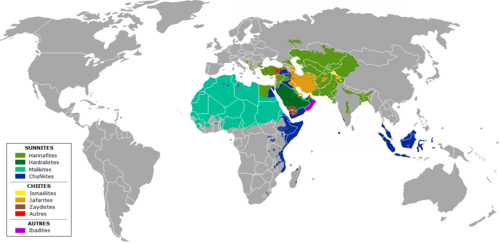
\includegraphics{Images/image097.png}
\vide{ruxe9ponse-soufie}{%
\subsection{Réponse soufie}\label{ruxe9ponse-soufie}}

Je vous propose de lire la lettre du Cheikh Ahmad al-Alawī
(1874-1934)~intitulée «~Lettre ouverte à celui qui critique le
soufisme~».

\vide{v--les-ordres-confruxe9riques}{%
\section{Les ordres
confrériques}\label{v--les-ordres-confruxe9riques}}

Il y en a une cinquantaine dans le monde.

\begin{itemize}
\item
  \textit{La qādirīya} \label{Def:Soufiqādirīya}
Fondateur~: `Abd al-Qādir al-Ğīlānī (m. 1166)
Implantation~: dans tous les pays musulmans, du Maghreb à la Chine


\item
  \textit{La Naqchabandīya} \label{Def:SoufiNaqchabandiya}
Fondée au milieu du XIV° siècle
Implantation~: du Caucasse au Turkestan et à l'Inde
Elle a nourri le nationalisme kurde


\item
  \textit{La Šāḏilīya} \label{Def:Soufisadiliya}
Eric Geoffroy dit de la \emph{Šāḏiliyya} qu'elle est l'une des
«~voies-mères~» du soufisme. Elle est apparue entre la fin du
XII\textsuperscript{e} siècle et le XIV\textsuperscript{e} siècle.
D'origine maghrébine, elle s'est diffusée au XIII\textsuperscript{e}
siècle, à partir de l'Égypte, dans la majeure partie du monde musulman.
Son enseignement est dense et il s'appuie sur les écrits d'Ibn
\emph{`}Arabī.
\end{itemize}
Toute voie initiatique a pour but de mener ses adeptes vers la sainteté,
ou «~proximité divine~» (\emph{walâya})~; celle-ci est identifiée au
plus haut degré de la gnose par al-Shâdhilî. De façon schématique, les
premiers maîtres shâdhilis distinguent deux niveaux~: la sainteté
«~mineure~» (\emph{sughrâ}), ouverte au public large des fidèles, et la
sainteté «~majeure~» (\emph{kubrâ}), réservée à une élite spirituelle.
Mais le terme \emph{walâya}, tout comme celui de sainteté en français,
est un terme générique, un idéal qui implique une méthode pour y
parvenir.

Pour les Shâdhilis, la réponse est claire~: c'est dans l'imitation
intérieure du Prophète que se réalise la \emph{walâya}. Réapparaît ici
le débat millénaire sur les rapports entre \emph{walâya}et
\emph{nubuwwa}, la prophétie, débats qui ont partagé exotéristes et
ésotéristes de l'islam, mais aussi les milieux soufis. Autant les
maîtres shâdhilis initiaux se réclament du premier théoricien de la
sainteté en islam, al-Hakîm al-Tirmidhî (m. 318/930), autant ils s'en
éloignent lorsque celui-ci accorde à la \emph{walâya}une autonomie par
rapport à la \emph{nubuwwa}~: pour eux, la première est subordonnée à la
seconde, et puise sa substance même dans la Lumière muhammadienne
(\emph{al-nûr al-muhammadî}).

\begin{itemize}
\item
  \textit{La Bekt'āchīya}
Elle impose le célibat
De nombreux affiliés en Turquie et Albanie


\item
  \textit{La Tidjānīya}
Influente au Maghreb et dans l'Afrique occidentale


\item
  \textit{La Chattārīya}
Influente en Inde et Malaisie

\item
  \textit{La Rah'mānīya}
La plus influente confrérie algérienne.


\item
  \textit{La mawlāwīya} (derviches)
\end{itemize}

Il existe plusieurs ordres soufis, mais l'on peut distinguer deux grands
groupes de mystiques~: ceux qui se trouvent dans la station de l'ivresse
(\emph{sukr}) et ceux qui sont dans la station de la sobriété
(\emph{sahw}).

Les initiés ivres sont souvent les disciples d'Abū Yazīd Bistamī (m.
875)~: l'ivresse, c'est la perte de sens commun, de la maîtrise de soi.
L'âme est enivrée de la connaissance de Dieu, plongée dans la
contemplation de Dieu.

Pour le second groupe, l'ivresse n'est qu'un état transitoire. Elle est
le début de l'unicité, mais elle se caractérise par la sobriété, quand
il sait que le soi n'est qu'un miroir dans lequel se réfléchit l'Essence
divine.

\paragraph{Pour aller plus loin}

Martin \textsc{Lings}, \emph{Qu'est-ce que le soufisme~?} traduit de
l'anglais par Roger du Pasquier, Paris, Éditions du Seuil, 1977.

Eric \textsc{Geoffroy},
«~\url{http://www.facebook.com/topic.php?uid=21148739744\&topic=3226}{L'islamité
du soufisme et son apport à la spiritualité universelle}~» dans
\url{http://www.religioperennis.org/documents/geoffroy/islamitesoufisme.pdf}

Eric \textsc{Geoffroy}, \emph{Initiation au soufisme}, Coll. L'espace
intérieur, Paris, Fayard, 2003.

Alberto Fabio \textsc{Ambrosio}, \emph{Vie d'un derviche tourneur}.
Doctrine et rituels du soufisme au XVII\textsuperscript{e} siècle,
Paris, CNRS Edition, 2010, 1 vol., 406 pages.

Laleh \textsc{Bakhtiar}, \emph{Le soufisme}. Expressions de la quête
mystique, Paris, Seuil, 1977.

Christian \textsc{Bonaud}, \emph{Le soufisme al-taṣawwuf et la
spiritualité islamique}, Préface de

Michel Chodkiewicz, Maison Larose, IMA, 1991.

\textbf{Exercice pour la Validation}

À partir de la lettre du šaḫy Ahmad al-Alawī, identifierez les éléments
qui répondent aux critiques adressées aux soufis et à Ibn `Arabī tels
que nous les avons exposés.



\chapter{Les racines de la réforme : le
renouveau islamique des XVIIe-XVIIIe
siècles}
\mn{(24/01/2022)}

Un leçon sur les racines de cette diversité, et de tous ces courants au sein du monde Sunnisme. Tout cela part du désir de "\textit{Réforme}" qui part à un retour au source. Et cela peut donner des solutions très diverses, soit des lectures libérales ou des lectures fondamentalistes (un peu comme les évangéliques protestants).
Plutôt \textit{Renouveau} que \textit{Réforme}.

%------------------------------------------------
\section{La crise interne du monde musulman}
\subsection{Déclin des grands empires}

 
 \begin{Synthesis}[Date Symbolique]
 1798 : Napoléon en Egypte, date symbolique de la rencontre du monde musulman avec la modernité occidentale.
 \end{Synthesis}
 Cette lecture n'est pas fausse et va donner lieu au \textit{réformisme} mais c'est une lecture occidentalo-centrée.
 En réalité, cela a commencé plus tôt. Un désir né courant XVII et interne au monde musulman.
 
Les trois grands empires musulmans de l'époque rentrent en crise : 

\begin{table}[h!]
    \sidecaption{Les trois grands Empires musulmans}


%\newlength\q
\setlength\q{\dimexpr .25\textwidth -2\tabcolsep}
\footnotesize%
\noindent\begin{tabular}{p{\q}p{\q}p{\q}p{\q}}
\toprule
                & Fondation           & Apogée                            & Fin                                                                                \\
\midrule
Empire Safavide & 1501 (Ismaïl   1er) & Abbas Ier (1588-1629)             & 1736                                                                               \\
Empire Moghol   & 1526 (Babur)        & Akbar (1556-1605)                 &  1857 (existence symbolique après 1761)  \\
Empire Ottoman  & 1299 (Osman 1er)    & Soliman le Magnifique (1520-1566) & 1922                                        \\
\bottomrule
\end{tabular}


    \label{tab:my_label}
\end{table}
 
 
\begin{figure}[h!]
    \centering
        \sidecaption{Empire Safavide, s'affaiblit
}
 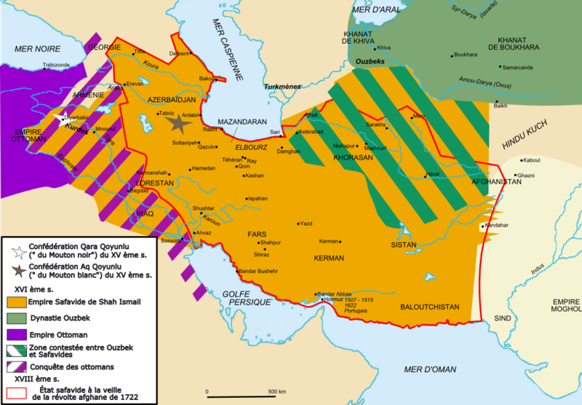
\includegraphics[width=0.9\textwidth]{CourantsIslamContemporain/ImagesCourantsIslamContemporain/empireSafavide.png}

    
\end{figure}


\begin{figure}[h!]
    \centering
        \sidecaption{Apogée et perte de l'empire Moghol : Au XVIII, il est réduit au Rajastan.
}
 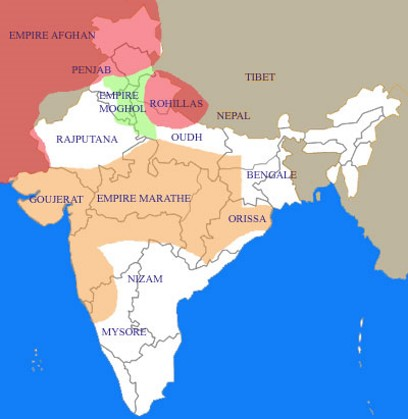
\includegraphics[width=0.44\textwidth]{CourantsIslamContemporain/ImagesCourantsIslamContemporain/Inde18.jpg}
  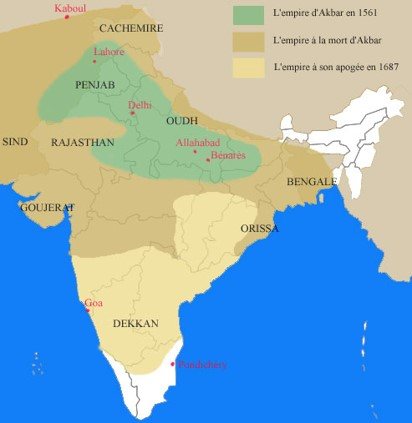
\includegraphics[width=0.44\textwidth]{CourantsIslamContemporain/ImagesCourantsIslamContemporain/empireMoghol.jpg}
\end{figure}

\begin{figure}[h!]
    \centering
        \sidecaption{Déclin Empire Ottoman
}
 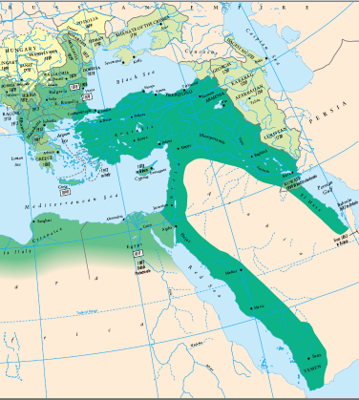
\includegraphics[width=0.5\textwidth]{CourantsIslamContemporain/ImagesCourantsIslamContemporain/declinEmpireOttoman.png}
\end{figure}
 
 \paragraph{Raisons économiques} Les portugais contournent l'Afrique et contournent les empires musulmans.  
 \paragraph{crises politiques} au sein de ces empires, trop grands. 
 \paragraph{Des voisins puissants} Ces Etats vont perdre des territoires face à des puissances qui ne sont pas musulmanes. L'empire Safavide est attaqué par les Ousbeks. L'Empire Moghol en XVIII siècle s'effondre devant l'empire Marathe (Hindou). L'empire Ottoman resiste mais décline depuis 1686 (siège de Vienne). 
 \begin{itemize}
     \item  {Affaiblissement des sultanats Indonésiens} face aux Hollandais. Java est annexé en 1800. 
  \item {En Chine} les musulmans Chinois (Hui) subissent des pressions des Manchous.
   \item  {Afrique} Les bambaras conquièrent Djenné, Tombouctou et Gao. Les portugais en Océanie. 
  \item {En Asie Centrale}, avancée des Russes (XIVII : Kazakstan et reste de l'Asie Centrale au XIX).
 \end{itemize}

 \paragraph{A la fin du XVI} 1591 : deuxième millénaire de l'Islam; sentiment millénariste. \mn{Calendrier lunaire, donc décalage}
 
 
 
\subsection{Problèmes doctrinaux et religieux}

\paragraph{Un raidissement des écoles juridiques au XVII}
Elles s'accusent les unes les autres de ne pas être juste, sentiment de division du monde sunnite.

\paragraph{Décadence du monde Soufi} On a tendance à considérer les soufis comme à la marge du monde musulman. Pourtant, elles ont joué un rôle social déterminant voire politique. Or, à l'époque, elles sont en crise.
\begin{itemize}
    \item {En faisant des Etats dans l'Etat} 
\item {Laxisme spirituel} Un soufi n'est plus tenu de suivre les prescriptions de l'Islam.
\item {Un rôle de plus en plus important du Sheykh}, le maitre spirituel de la Confrérie, qui transmet la \emph{Baraka}.
\item {Des pratiques spéctaculaire} Le fakirisme. le \emph{Dhikr}, rappel du nom de Dieu et l'on atteint l'Etat de transe, et vont marcher sur des braises. 

\end{itemize}



%------------------------------------------------
\section{L'aspiration au
  renouveau}
\subsection{Millénarisme}


 \begin{Def}[rapport au temps Involutif]
 L'Islam se tourne vers le passé, en Islam, les prophètes viennent toujours rappelés ce qui a été donné à l'origine. et le problème est que les hommes déforment le message transmis. Donc Dieu envoie de nouveaux prophètes pour restaurer le message originel. \textit{le temps corrompt.}
 
 \end{Def}
 vs Evolutif. 
 
 Ce qui fait que Mohammad est le dernier des prophètes, c'est que le message est transmis intact, pour la première fois, donc plus besoin de nouveaux prophètes. Autant, la \textit{pratique} peut se corrompre. 
 Un hadith dit : 
 \begin{quote}
     Slt un dixième de la pratique suffira pour sauver le monde.
 \end{quote}
 
 \begin{Def}[Moujaddid]
 de la racine JDD, nouveau, celui qui renouvelle l'Islam pour le mettre tel qu'il était à l'origine. 
 \end{Def}

 
 \begin{Def}[tajdid]
 Tajdid, le renouveau, qui doit venir régulièrement. Chaque siècle Dieu envoie un \textit{Moujaddid} selon un Hadith du Prophète.
 \end{Def}
 
 
 Il peut y en avoir plus mais à chaque siècle, il y a un grand moujaddid, savant, qui ne fait pas forcément au sein de la communauté. 
  \begin{Ex}
 Ghazali est considéré comme un Moujaddid
 \end{Ex}
 \sn{On retrouve cette tension dans toute religion entre respect de la forme et de fidélité au message d'origine}
 
 \subsection{Quelques grandes figures de la \textit{pre-Reforme}}
 

\paragraph{Ahamad Sirhindi} (Inde, 1564-1624) , essaye de rénover l'Islam et réforme une confrérie, la \emph{Naqshbandiyya} réformée (mujaddidi). 
\paragraph{Muhaddidi} Restaurer le monde musulman et restaurer l'Islam dans sa pureté originelle. Il va opposer 
\begin{itemize}
    \item le \emph{taqlid}, l'imitation (péjorative, servile, non réfléchie) et
    \item l'\emph{ijtihad}, l'effort d'interprétation du Coran et de la Sunna. Retourner aux sources scripturaires pour restrouver le sens authentique de l'Islam
    \item pour éliminer la \emph{bid'a}, très péjoratif, l'innovation
\end{itemize}  

On peut distinguer deux courants : un courant plus libéral et l'un plus fondamentaliste :
\begin{itemize}
    \item le rapport à la Tradition : fondamentaliste ne vont considérer que le Coran et la Sunna, en critiquant les élaborations savantes de l'Islam. 
    \item ce sur quoi va porter l'\emph{ijtihad}, soit limité sur les versets peu clairs du Coran, soit plus large pour le savant et les différentes sciences qui vont être convoquées pour l'ijtihad.
\end{itemize}


\paragraph{Muhammad 'Abd Al-Wahhab } 'Arabie, 1703-1792). Voir p. \pageref{Theol:AlWahhab}

\paragraph{Shah Wali Allah} (Inde, 1703-1762), \label{Theo:waliAllah} a eu les mêmes professeurs que Al-Wahhab ! et l'un des premiers à traduire le Coran dans une langue vernaculaire (en persan). Effort d'acculturation dans le contexte Moghol et Indou. 




 
%------------------------------------------------
\section{Les voies du renouveau} 
\subsection{Les confréries soufies}

La création de néo-confrérie
\begin{itemize}
    \item lutter contre un laxisme moral
    \item lutter contre le pouvoir du Sheykh.
    \item insister sur le côté social, en prenant en charge la société (vs gnosticime ?).
\end{itemize}
\mn{Soufi : \pageref{Def:SoufiNaqchabandiya}, \pageref{Def:Soufiqādirīya} }




\paragraph{Ahmad Al Tijani} (Algérie 1737, 1815). Et fonde la \emph{\textbf{tijaniyya}}, un groupe toujours très présent en Afrique du Nord. Normalement un Sheykh insiste sur la chaine d'initiation qui remonte au prophète. Lui, va être initié directement en rêve par le Prophète.

\paragraph{Abdurrauf al-Singkili} (Aceh, Indonésie, 1615-1693)

\paragraph{Abdelkarim al-Samman} (Soudan, 1718-1776) => sammaniyya

Au sénégal, aussi une confrérie de type réformée. 
\mn{A completer carte Carte moderne. Il y avait 24 confréries soufis en Arabie avant le Wahhabisme}




%---------------------------------------
\subsection{Les centres de pèlerinage : La Mecque et Médine}

La Mecque et Médine jouent un rôle essentiel, du fait du Hajj. Du fait de l'Empire Ottoman, il y a pacification des parcours du pélerinage, par ailleurs incités par l'Empire.
Et par ailleurs, des centres de formation s'implémentent à la Mecque.  On en profite pour étudier. Se croisent des savants de différentes origines.
Non seulement les centres d'étude mais aussi les confréries, avec leur Sheykh les plus importants s'installant à Médine ou la Mecque. Ils sont initiés à l'enseignement Moujaddidi et vont réformer la confrérie à laquelle ils appartiennent, selon un modèle qui se répète.




%------------------------------------------------
\section{Un aspect particulier : les jihads aux marges du monde   musulman} 


\begin{figure}[h!]
    \centering
        \sidecaption{Le « renouveau » des marges du monde musulman (XVIIIe-XIXe
siècle)  \emph{L'atlas de l'islam depuis 1500}, F. Robinson, Nathan, 1987  
Des petits Etats vont se créer sur des bases confrériques et dont la mission de faire le jihad.
}
 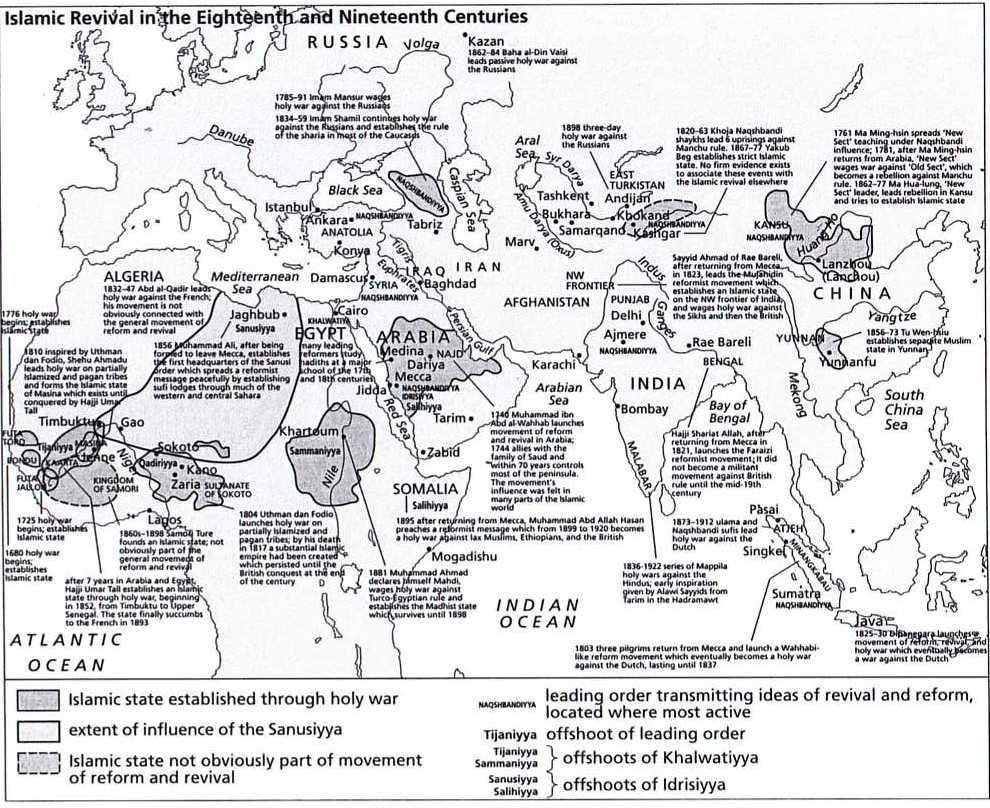
\includegraphics[width=\textwidth]{CourantsIslamContemporain/ImagesCourantsIslamContemporain/image1.jpeg}

    \label{fig:le-renouveau-des-marges-du-monde-musulman-xviiie-xixe-siuxe8cle}
\end{figure}


\subsection{Situation particulière des zones marginales}


Pourquoi on les retrouve aux marges du monde musulman ? Il y a un besoin de purification et l'islamisation par rapport à des populations hétérogènes. Mais aussi, parce que ces zones ne sont pas controlées par les grands empires musulmans qui ne tolèrent pas ces confréries.
Le jihad se porte d'abord sur les musulmans eux-mêmes, pour qu'ils deviennent musulmans puis contre les puissances extérieures ou non musulmanes qui controlent ces zones. 

\paragraph{Une structure Etatique} Le Sheykh est le chef, \emph{Commandeur des Croyants} - on fait référence aux premiers temps musulmans, on prête allégeance, et avec une approche puritaine, très forte pratique. \mn{Des analogiques avec DAESH, qui se réfèrent eux aussi aux temps de l'Islam}

\paragraph{Une accélération de l'Islamisation}


\subsection{Quelques exemples}

\paragraph{Spectre Temporel 1680-1920}{1680, Etat de Bondou} Afrique de l'Ouest jusqu'e l'Etat Mahdiste (Somalie) 1899-1920.

\paragraph{Chine - Ma Ming-hsin} Réveil religieux des communautés chinoises sous la pression des Manchous. Ma Ming-hsin (1719-1781) lorsqu'il est à la Mecque, il fonde une confrérie réformée, la \textit{Nouvelle Secte} et entre en opposition contre les autorités locales, qui appelle en soutien la dynastie Manchoue des Ming. Ming-Hsin est décapité. Il y aura d'autres révoltes plus tard, du Kan-Su et du Chen-Si (1862) et du Yunnan (1856)

\paragraph{Indonésie - Jajji Miskin} Le mouvement Padri à Sumatra (1803-1845). Après le Hajj, en 1803, il prend le contrôle de villages et va imposer sa vision de l'Islam, interdit les pratiques populaires et proclament le Jihad contre les autres villages et les pouvoirs. 1820 : les Hollandais reviennent dans la région et on a une transformation de ce mouvement contre un Jihad contre les Hollandais. Eliminé par les Hollandais.

\paragraph{Nigéria - Califat de Sokoto} Uthman da Fodio (1755-1817) issu d'une famille de savants musulmans, l'enseignement lui vient par la fraderyya\sn{revoir} et crée une communauté qui le reconnait comme \textit{commandeur des Croyants}, s'oppose aux pouvoirs locaux et va être défait par la Grande Bretagne.


\begin{Synthesis}
\begin{itemize}
Ce renouveau : 
    \item Avant la rencontre de l'Occident
    \item lié à des thèmes de crises internes
    \item des thématiques que l'on retrouvera : retourne aux sources scripturaires
    \item C'est assez fascinant de voir la circulation des idées, liée autour du \textit{Hajj}
\end{itemize}


\end{Synthesis}

%------------------------------------------------

 



 



\paragraph{Soufis du Badakhshân : un renouveau confrérique entre
l'Inde et l'Asie centrale}
\mn{Alexandre Papas, \emph{Cahiers d'Asie Centrale}, n° 11-12, 2004, p.
87-102 (extraits -- texte expurgé)}
 
 
\subparagraph{Éléments de biographie d'un soufi
badakhshânais} 
\mn{le Badakhshân est entre l'Afghanistan et le Tajikistan}
\begin{quote}
Mawlânâ Mîr Ghiyâs al-Dîn \label{Theo:MawlanaMirGhiyasAlDin} naît en 1117/1705-06 dans la petite localité
de Hisârak, située au cœur du district de la ville de Jirm. Le
grand-père de Mawlânâ a émigré du village de Dahbîd, non loin de
Samarcande, en direction du Badakhshân. La \emph{silsila}\sn{Génération} de la famille
remonte au Prophète et, sur dix générations, au frère d'un grand saint
Kubrawî et découvre une généalogie \textit{soufie}. C'est donc au sein d'une des
grandes familles \emph{muhâjir}\sn{Emigré, en référence aux premiers musulmans qui ont suivi le Prophète à Médine} de l'aristocratie religieuse du
Badakhshân que naît Ghiyâsî.
\begin{figure}[h!]
    \centering
        \sidecaption{Asie Centrale. On oublie parfois le rôle important de ces états tampon comme lieux d'échange
}
 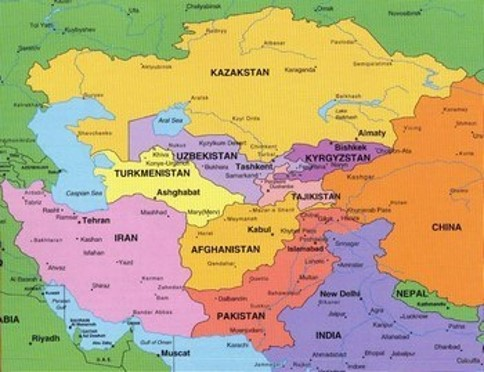
\includegraphics[width=\textwidth]{CourantsIslamContemporain/ImagesCourantsIslamContemporain/AsieCentrale.jpg}
 
\end{figure}

{[}\ldots{]}

C'est précisément pour l'Inde -- destination qui concurrence la
Transoxiane savante, en particulier Boukhara, surtout depuis le XVIe
siècle -- que part le jeune Ghiyâsî âgé de 14 ans en quête d'initiation \sn{soufi}.
Cet exil de l'adolescent fait l'objet de deux contes hagiographiques :
 

\begin{itemize}
\item
 
  Le futur shaykh de Ghiyâsî, Shâh Walî Allâh, qui a quitté Sirhind pour
  entreprendre un pèlerinage au mausolée de Bahâ' al-Dîn Naqshband\sn{le fondateur de la confrérie réformée Naqshandayyi} non
  loin de Boukhara, stationne au Badakhshân, à Jirm, chez le père même
  de Ghiyâsî. Le shaykh demande alors à ce dernier de lui amener ses
  enfants, mais perçoit par claire-vue qu'on lui dissimule le jeune
  Mawlânâ qui, en état de \emph{majzûb}\sn{Ils peuvent faire des choses indécentes} « ravi en Dieu », suscite la honte de
  sa famille. À sa vue le shaykh indien cite un vers de Ni'mat Allâh
  Walî Kirmânî. Et au jeune Ghiyâsî de prononcer miraculeusement le
  second vers du distique. Walî Allâh annonce alors qu'à son retour de
  Boukhara il prendra le jeune homme comme disciple et l'emmènera en
  Inde.
  
\item
 
  Dès l'âge de 9 ans Mawlânâ refuse les conseils de sa famille et se
  distingue des autres enfants. Plusieurs nuits, au cours de rêves, lui
  apparaît un homme illuminé qui lui enjoint de partir pour l'Inde où
  lui est promise la rencontre d'un grand saint soufi. Malgré le refus
  de ses parents qui souhaitent marier leur fils, Ghiyâsî parvient à
  quitter le Badakhshân quelques années plus tard. Parvenu à Lahore et
  après un nouveau rêve révélateur, il attend de nombreux jours au
  couvent de Khwâja Khwândamîr, un khalîfa de la Naqshbandiyya, jusqu'au
  jour où il rencontre Shâh Walî Allâh.
 
\end{itemize}

 
Restent les faits : après une formation classique en \emph{madrasa} à
Delhi où le novice rencontre ses premiers maîtres, il devient à Lahore
durant douze années le disciple d'un fameux maître Naqshbandî Mujaddidî.
Il interrompt une unique fois son initiation lorsque le shaykh lui
confie la mission de se rendre au Cachemire afin d'aller chercher un
homme qu'on prétend thaumaturge et que Walî Allâh souhaite convertir à
l'islam et initier à sa \emph{tarîqat}\sn{confrérie}. Au terme de ses douze années de
noviciat, le shaykh lui enjoint de retourner à sa terre natale pour
propager la confrérie. De retour au Badakhshân, Ghiyâsî âgé de trente
ans environ et qui a obtenu le rang de \emph{mawlawiyyat}\sn{maître}, fait office
d'enseignant à la \emph{madrasa} Jâmi'-i Islâmî du district de Jirm. Il
est ensuite convié à Fayz Âbâd à la cour de Sultân Shâh, laquelle abrite
des savants et des poètes venus d'Inde et d'Iran, dont certains
acquièrent grande réputation. C'est là que Ghiyâsî compose son œuvre
poétique et mystique. C'est également là, de son \emph{khânaqâh}\sn{couvent soufi, Ḵānqāh ou ḵānāqāh, fut d'abord un lieu destiné à abriter les spécialistes et savants religieux musulmans (‘ulamâ’), une sorte d'équivalent des couvents chrétiens. Ces établissements ont été ensuite réservés aux soufis.}, qu'il
dirige son enseignement, suivis par de nombreux disciples venus de
toutes les régions alentours. Le soufi badakhshânais devient aussi le
directeur spirituel de Sultân Shâh. Et lorsque ce dernier est capturé à
Qunduz par les ouzbeks du Qataghân en 1179/1765, le vieux maître
conseille durant trois ans le fils et suppléant du shah emprisonné, Mîr
Muhammad Shâh. D'un tel succès et d'une telle influence, Ghiyâsî
apparaît comme l'un des principaux promoteurs de la Mujaddidiyya dans le
Nord de l'Afghanistan.

{[}\ldots{]}
\end{quote}

\begin{Prop}
On retrouve des noms : Walî Allâh (cf p. \pageref{Theo:waliAllah}; l'importance du réseau confrérique; et rôle social (il devient le conseil du sultan).
\end{Prop}

\subparagraph{Savants et soufis au croisement du
Badakhshân}
Le Pamir est un sanctuaire pour les savants hétérodoxes ou bannis (cf Unwân banni d'Egypte du fait de sa lutte sociale).

\begin{quote}
Malgré les obstacles géographiques et en dépit des troubles politiques
qui affectent la fin du XVIII\textsuperscript{e} siècle, le Badakhshân
reçoit la visite de savants religieux qui, pour certains, décident de
s'y installer et interrompent définitivement leur voyage vers l'Inde ou
vers la Transoxiane. Il faut rappeler ici que le Pamir a, de façon
continue dans l'histoire, servi de sanctuaire à des individus frappés
d'ostracisme ou fuyant la répression dans leur région natale. Mais au cours du
XVIII\textsuperscript{e} siècle le sanctuaire se mue en lieu de
renaissance où fleurissent \emph{madrasa}\sn{lieu d'enseignement religieux} et couvent soufis. Le
\emph{Armaghân-i Badakhshân} mentionne le cas de deux étudiants de
Peshawar, Mîr Ahmad Mujaddidî dit `Izhâr' (m. 1259/1843) et son frère
Muhammad Anwar qui, à une date indéterminée durant le règne de Mîr
Muhammad Shâh, se rendent d'abord à Boukhara afin d'obtenir les
compétences du rang de \emph{`âlim}\sn{savant} et qui, lors de leur retour,
s'installent et officient au Badakhshân, pour le premier à Jirm, pour le
second à Bahârak.

Un autre cas de figure est celui, analogue à Ghiyâsî, de ces
badakhshânais qui partent se former aux sciences religieuses, et
éventuellement au soufisme, dans les grands centres de savoir du monde
musulman, proches ou lointains. De ce point de vue, le cas le plus
intéressant -- et malheureusement le plus douloureux faute
d'informations suffisantes et dans l'absence de vestiges de son œuvre --
est celui de Sayyid Abâ al-Hasan « `Unwân ». Né à Jirm en 1123/1711, il
quitte le Badakhshân pour Boukhara afin d'acquérir une formation
théologique. De là `Unwân se rend au pèlerinage de La Mecque et à
Médine, puis il s'installe durant 18 ans en Egypte, probablement au
Caire, où il poursuit son acquisition des sciences islamiques classiques
et commence à enseigner. Mais `Unwân ne se contente pas de dispenser un
enseignement religieux, il prend parti pour les classes populaires
égyptiennes et contre leur oppression par les propriétaires terriens.
C'est du moins la réputation qu'il gagne selon le \emph{Armaghân-i
Badakhshân}, et qui lui vaut d'être banni d'Egypte. `Unwân part alors
pour Istanbul, rejoint Boukhara et reprend son enseignement. `Unwân, qui
prône l'unité de la Communauté des Croyants (\emph{umma}), décide
d'aller prêcher la concorde (\emph{âshtî}) dans le Caucase, peut-être au
moment de l'activisme Naqshbandî de Shaykh Mansûr dans les années 1780.
Mais il renonce à son projet et entre dans une retraite spirituelle
jusqu'à sa mort en 1206/1791, sans être retourné au Badakhshân.
{[}\ldots{]}

\end{quote}

\begin{Prop}
 Dans le deuxième paragraphe, `Unwân se forme à la Mecque et Médine (rôle du pélerinage), rôle social en Egypte et pas seulement religieux. L'importance aussi de l'Unité, l'\textit{Umma}. 
\end{Prop}
 
\subsection{Liste des neo confréries}

\paragraph{Naqshbandiyya}: La Mecque, Damas, Yémen, Inde, Asie Centrale \label{Def:Naqshbandiyya}
                     => Caucase, Chine Occidentale + Orientale, Sumatra.

\paragraph{Qadiriyya}: Proche Orient, Irak, Inde, Asie centrale 
                    => Indonésie (Java, Aceh), Caucase, Afrique

\paragraph{Khalwatiyya}: Egypte => nombreuses branches en Afrique :

\begin{itemize}
    \item \textit{Tijaniya}: Algérie => Afrique de l’Ouest
    \item \textit{Sammaniyya}: Soudan
    \item \textit{Idrisiyya}: Maroc => Sanusiyya (Lybie), Sahiliyya (Somalie),
    \item \textit{Murghaniyya} (Erythrée)
\end{itemize}- 
 
%-----------------------------------------------
\subsection{bibliographie}

\begin{quote}


AZRA, Azyumardi \emph{The Origins of Islamic Reformism in Southeast
Asia}, Asian Studies Association of Australia/KITLV Press, Leiden, 2004.

PAPAS, Alexandre \emph{Soufisme et politique entre Chine, Tibet et
Turkestan}, J. Maisonneuve, Paris, 2005.

*ROBINSON, Francis \emph{Atlas de l'Islam depuis 1500}, Nathan, Paris,
1987 (dispo à la FELS)

*VOLL, John R. « Foundation for renewal and reform », in John L.
Esposito ed., \emph{Oxford History of Islam}, Oxford University Press,
1999, pp. 509-547.
\end{quote}
\chapter{Un fruit du « pré-réformisme » : le wahhabisme}
\mn{ \emph{(31/01/2022)}}

%---------------------------------------------------------
\section{Le wahhabisme}
\paragraph{Pourquoi en parler} C'est un courant qui a presque trois siècles, avec une évolution dans le monde du musulman qui a évolué. Il faut penser l'Islam contemporain dans son contexte.

 
  \subsection{Muhammad Ibn al Wahhab
  (1702-1792)} 
  \label{Theol:AlWahhab}
  
\paragraph{Origine} Son père est \emph{qadi}\sn{juge} et enseignant. Dans le Hadz. Fait un pélerinage à la Mecque. Renouveau

\paragraph{Formation et premières prédications} Proclame le \emph{Tawhid} l'unicité et lutte contre toutes les pratiques "déviantes". Il se heurte aux autorités locales et retourne donc à la Mecque. Il se forme là avec des maîtres d'Arabie et Indien. Puis se rend à Basra, à un autre maître. C'est là qu'il rencontre les si'ites. Il se heurte de nouveau aux autorités locales. Il rentre en Arabie mais \textit{son père y est hostile}. Ce n'est pas un grand savant mais un lettré. 
 
\paragraph{L'alliance avec Ibn Se`ud} Alliance matrimoniale avec un chef de tribu de la Mecque. Il se rend indésirable et il est obligé de partir et il arrive dans le village de Dariya et il y rencontre un autre chef de village, Mohammed Ibn Se'ud, alliance elle aussi politicolo-religieuse et matrimoniale en 1744. Ibn Se'ud accepte la doctrine et al Wahhab légitime l'acquisition de terre par Ibn Se'ud. 

Wahhab enseigne beaucoup  : il écrit beaucoup à des savants (\emph{Oulema}) à l'intérieur et l'extérieur du royaume de Ibn Se'ud. \textit{selon un modèle prophétique}, Mohammad ayant écrit au Basileos,... 

\paragraph{Un développement politique} Conquiert toute l'Arabie Saoudite. En 1818, c'est la fin du premier état wahhabite car l'empire ottoman intervient et execute le fils de Ibn Se'ud.
    
 Il s'appuie sur deux auteurs : 
\begin{itemize}
    \item Ibn Taymiyya (1263-1328), \label{Theol:Taymiyya2} \sn{cf p. \pageref{ibn-taymiyya}}, un vrai penseur
    \item Ibn Qayyim (1292-1350) un de ces disciples
\end{itemize}
 
Ibn Wahhab insiste sur le retour à la source mais en fait il lit le Coran à travers ces deux auteurs.

\paragraph{Une doctrine condamnée} Son père et son frère s'opposent à lui. Une fatwa contre lui du fait de sa critique sur les différentes écoles juridiques et le fait qu'il exclut de la communauté musulmanes ceux qui ne pensent pas comme lui. 

  \subsection{La doctrine wahhabite} 



  \paragraph{Nécessité du retour aux sources} Accentuation des sources, bien sûr le Coran. 
  \begin{itemize}
      \item  \item  Wahhab s'éloigne d'une lecture du Coran ligne à ligne mais propose une analyse \textit{thématique}.
  \item Il rejette aussi le besoin d'une \textit{médiation} humaine pour comprendre le Coran. Il s'oppose aux \emph{Ashraf}, les descendants du prophète \sn{Les Ashrafs ont un statut particulier dans l'Islam} ainsi qu'aux \emph{Imams} dans le si'isme, ainsi que les \emph{sheykhs} soufis.
  \begin{Prop}
  Il n'y a pas besoin de sciences particulières pour accéder au sens du Coran, d'après Wahhab. 
  \end{Prop}
  \item il suis les \emph{Hadiths}, la seule exégèse possible, la \textit{sunna} et rejette les grands commentaires classiques du Coran.  Cela va jusqu'à critiquer la tradition des 4 premiers Califes \textit{bien guidés}. Abu Bakr avait détourné la \textit{zakat} pour ses propres dépenses.
  \item Il reprend la distinction d'Ijtihad, qu'il limite aux versets aux versets obscures, contre le taqlid. Il s'oppose à deux principes de l'Ijtihad : qiyas (recours par analogie : alcool et drogue), \textit{ijama} (consensus des savants : on considère que cela fait autorité \sn{Infaillabilité de la communauté dans les Hadiths}), et le \textit{ra'y}, l'opinion personnelle du juriste. 
  
  \end{itemize}
 
 \begin{Prop}
 Il conteste les principes sous-jacents aux savants qui l'ont précédés. Il y a une tension entre son ambition de revenir au Coran mais en parallèle en se mettant en filiation avec Ibn Taymiyya
 \end{Prop}
 
 
  \paragraph{Une notion centrale : le \emph{tawhid} (unicité divine)}
  
  \mn{{Extraits du \emph{Kitab at-tawid} (Livre de
l'unicité divine) de Muhammad Ibn Wahhab} . {Chapitre 1} : \emph{Tawhid}
Traduction et édition établies en Arabie Saoudite. Allah est traduit par Allah et non Dieu, alors qu'en Arabe, Dieu est traduit par Allah y compris pour les chrétiens arabes. }

\begin{quote}
\emph{Allah-ta`ala} a dit : « Je n'ai créé les djinns et les hommes que
pour qu'ils M'adorent (1 :56)\ldots Et très certainement nous avons
suscité dans chaque communauté un message pour leur dire d'adorer Dieu
et d'écarter le Rebelle (16 :36)\ldots Et voilà que ton Seigneur a
décrété que tu dois n'adorer que Lui et faire preuve de bonté envers tes
parents (17 :23)\ldots Adorez Dieu et ne lui donnez quelque associé que
ce soit (4 :36)\ldots Venez, je vais vous réciter ce que votre Seigneur
vous a interdit ; - ceci : Ne lui associez quoi que ce soit\ldots(6
:151-153) ». Ibn Mas`ud a dit : « Quiconque se propose de vérifier le
testament du Prophète Muhammad (SWA) -- un testament sur lequel le
Prophète a apposé son sceau, qu'il lise ces mots d'Allah : « Venez, je
vais vous réciter ce que votre Seigneur vous a interdit ; - ceci : Ne
lui associez quoi que ce soit\ldots Voilà ce qu'il enjoint » (6 :
151-153)


Mu`adh Ibn Jabal raconta : « Je montai derrière le Prophète (SAW) quand
il me dit : « Ô Mu`adh ! Sais-tu ce que les créatures d'Allah Lui
doivent et ce qui leur est dû ? » Je répondis : « Allah et son Prophète
savent mieux ». Il continua : « Ce que les créatures d'Allah Lui
doivent, c'est de ne jamais associer qui que ce soit avec Lui. Ce qui
leur est dû, c'est qu'il ne punira aucune personne qui ne Lui associe
pas un autre ». Je dis :

« Ô Prophète d'Allah, est-ce que je peux annoncer la bonne nouvelle aux
gens ? » Il répliqua : «Non ! Ne leur dis rien de peur qu'ils comptent
sur la promesse et manquent à leurs devoirs envers Lui». Ce hadith est
mentionné dans deux \emph{Sahihs}.


D'autres points :


\begin{enumerate}

\item
  \begin{quote}
  La sagesse dans la création du djinn et de l'humanité.
  \end{quote}
\item
  \begin{quote}
  Le service à Allah consiste en le \emph{tawhid}. Car, à l'opposé du
  \emph{tawhid} se trouve l'aliénation d'Allah. (\ldots)
  \end{quote}
\item
  \begin{quote}
  La sagesse d'envoyer des prophètes. (\ldots)
  \end{quote}
\end{enumerate}
  \end{quote}
  
On trouve une accumulation de versets coraniques sur le thème, puis des hadiths du prophète. Le grand péché par excellence, c'est le \emph{shirk}, l'associationisme des Dieux à Dieu. Or Wahhab va plus loin. 

\begin{quote}


\emph{Allah-ta`ala} dit : « Ceux qui ont cru et n'ont point revêtu de
prévarication leur foi\ldots{} » (6 : 82).

(\ldots) Abu Sa`id al Khudriyy rapporta que le Prophète d'Allah (SWA) a
dit : « Quand Musa {[}Moïse{]} demanda à Allah de lui enseigner une
prière qu'il puisse réciter à chaque fois qu'il pensait à Lui ou qu'il
L'évoquait, Allah répondit : « Dis, ô Musa, qu'il n'y a d'autre Dieu
qu'Allah. Musa dit : « Ô Seigneur, tous tes serviteurs prononcent ces
mots ». Allah dit : « Ô Musa, si les sept cieux et tout ce qu'ils
renferment, et les sept terres aussi, si tout cela était pesé contre
cette phrase : « Il n'y a d'autre Dieu qu'Allah », cette dernière
pèserait plus lourd ». Ibn Hibban rapporta cela également et al-Hakim
compléta sa version. Al-Tirmidhi enregistra, avec peu de rédaction, le
récit de Anas à l'effet qu'il entendit le Prophète d'Allah (SWA) dire :
« Allah dit : « Ô Homme ! Si tu venais à Moi avec tous les sacs du monde
remplis de tes péchés, mais avec le témoignage que tu n'associes rien à
Moi, Je viendrais à toi avec tous mes sacs remplis de miséricorde et de
pardon ! ».

    
\end{quote}

\begin{Synthesis}
Si on respecte le \emph{Tawhid}, cela suffit à pardonner les péchés, mais important de respecter les principes de l'Islam (c'est pour cela que c'est caché)
\end{Synthesis}

\paragraph{Distinction au sein du Tawhid } 
\begin{Def}[Le grand Shirk ]
Il distingue le \emph{tawhid rububiyya} (l'unicité de souverainté du monde) avec le \emph{tawhid uluhiyya} (de divinité) : ne reconnaitre aucun intermédiaire entre Dieu et les hommes. Il ne peut y avoir de dévotion que pour Dieu seul : les saints, les soufis, les Imams.
\end{Def} 
Al Wahhab introduit une critique fondamentale contre le soufisme. 

\paragraph{Le petit Shirk} 
\mn{{Chapitre 4} : La crainte du \emph{shirk}}
\begin{quote}
Allah -- qu'Il soit loué et glorifié -- dit : « Non, Dieu ne pardonne
pas qu'on Lui donne quelque associé. En deçà, Il pardonne à qui il veut
» (4 : 48, 116)

(\ldots) Dans le hadith, nous lisons : « Ce que je crains le plus pour
vous, c'est le moindre \emph{shirk}. Quand on lui demanda ce que
c'était, le Prophète répondit : « l'hypocrisie ». Dans le Sahih
d'al-Bukhari, nous lisons que Ibn Mas`ud reporta : « Le Prophète d'Allah
(SWA) a dit : « Celui qui rencontre Allah le jour du Jugement sans Lui
avoir associé qui que ce soit ira au Paradis, et celui qui le rencontre
ayant fait le contraire sera consigné en Enfer ».
\end{quote}
\begin{Def}[le Petit Shirk]
Toute attitude de l'homme qui ne sert pas Dieu. il relève aussi de l'attitude morale.
\end{Def}

\begin{Ex}[L'appel à témoigner qu'il n'y a d'autre
Dieu qu'Allah]

\mn{{Chapitre 5} : }
\begin{quote}
\emph{Allah-ta`ala} a dit : « Dis (ô Muhammad) : `\,`Voici mon sentier,
j'appelle à Dieu'\,' » (12 :108)

Ibn `Abbas (RA) rapporta : « Quand le Prophète d'Allah (SAW) envoya
Mu'adh à al-Yaman, il lui recommanda : `\,`Quand tu rencontres des gens
du Livre, que ta première action soit de leur demander de témoigner
qu'il n'y a d'autre Dieu qu'Allah'\,' ». Selon un autre récit, «
\ldots{} de leur demander de réaliser l'unicité d'Allah. S'ils
t'obéissent, informe-les qu'Allah leur a imposé la \emph{salat} cinq
fois par jour. S'ils t'obéissent en cela, alors informe-les qu'Allah
leur a imposé le devoir de charité qui doit être perçue des riches pour
être distribué aux pauvres. S'ils t'obéissent en cela, ne touche pas à
leurs autres biens et occupe-toi de la plainte de l'opprimé, car il n'y a aucun obstacle dans son accès à Allah ».
(Rapporté dans les \emph{Sahihs} d'al-Bukhari et de Muslim). (\ldots)
\end{quote}
\end{Ex}



\paragraph{Les Intercessions} L'intercession est limitée à Mohammed, et uniquement aux musulmans suivants Wahhab. On ne peut pas prier le Prophète. Peut être intervient-t-il au jugement dernier.


\mn{{Chapitre 17} : L'intercession}
\begin{quote}
Allah -- qu'il soit loué et glorifié -- a dit : « Et par ceci (le
Qur'an), avertis ceux qui, n'ayant pour eux hors de Dieu, ni ami ni
intercesseur, craignent d'être rassemblés vers le Seigneur\ldots{} » (6
: 51). Dis : « A Dieu l'intercession tout entière\ldots{} » (39 : 44).
Qui peut intercéder auprès de Lui que par sa permission ?... (2 : 255).
Et combien d'anges dans les cieux ? Leur intercession ne met au large en
rien, sauf après que Dieu l'a permis, en faveur de qui il veut et qu'il
agrée » (53 : 26). (\ldots)

(\ldots) En tant que catégorie générale du Jour du Jugement en laquelle
les mécréants croient, l'intercession est rejetée par le Qur'an. Le
Prophète (SAW) nous informa qu'en ce jour « il sera amené devant Allah.
Il se prosternera lui-même et louera Allah, plutôt que de demander à
intercéder. Alors on lui dira : « Lève-toi ! Parle maintenant et tu
seras entendu ! Demande et il te sera donné ! Intercède et il te sera
accordé ! » (\ldots) L'intercession est donc là pour les croyants
sincères et candides. Elle n'est accordée que par la permission d'Allah
et n'appartient pas aux associationistes. (\ldots)
\end{quote}


\paragraph{Tombe du juste}
Condamnation de celui qui invoque Dieu
auprès de la tombe du juste et, a fortiori, de celui qui invoque ce
dernier.
\begin{Ex}[Un exemple de Grand Shirk]
\mn{{Chapitre 20} : Condamnation de celui qui invoque Dieu
auprès de la tombe du juste et, a fortiori, de celui qui invoque ce
dernier.}
\begin{quote}
Dans le \emph{Sahih}, A'ishah (RAA) rapporta : « Umm Salmah raconta au
Prophète d'Allah (SAW) qu'elle avait vue une église remplie d'images et
de statues en Abyssinie. Le Prophète dit : « Ceux-là sont les pires de
tous les hommes : lorsqu'un membre juste et vertueux de leur groupe
meurt, ils bâtissent une église sur sa tombe et y installent toutes
sortes d'images pour lui. Ils sont coupables de deux méfaits : celui
d'invoquer quelqu'un auprès d'une tombe et celui d'installer des images
». (\ldots)

Ainsi le Prophète interdit cette pratique et condamna celui qui la
suivait. Faire le \emph{salat} sur une tombe est également interdit,
même si aucune mosquée n'a été construite sur l'emplacement. Telle est
la signification de la déclaration suivante : « On craignait qu'elle ne
soit prise pour une mosquée ». Les Compagnons n'étaient pas supposés
construire une mosquée autour de la tombe du Prophète. Tout endroit
destiné au \emph{salat} ou tout endroit où le \emph{salat} est accompli,
est une mosquée. Tel l'a déclaré le Prophète (SAW) : « Toute la terre
est pour moi une mosquée, un endroit pur (pour accomplir le
\emph{salat}) ».
\end{quote}

\end{Ex}


  \paragraph{La question du \emph{jihad}} La question de la violence chez Wahhab. Il faut repartir de la position kharijite. Un calife doit respecter la religion de façon exemplaire. s'il ne le fait pas, il est \emph{Takfir}, mécréant. Or la vision sunnite a jugé que c'est Dieu uniquement qui jugera si un musulman est un non-musulman. Ibn Taymmayyia s'élève contre les souverains Mongols : : les souverains mongols sont certes musulmans puisqu'ils ont adopté la foi musulmane mais en surface.  Wahhab va reprendre ce concept et ceux qui n'adhèrent par au \emph{shirk} sont apostats. Un germe de violence.
  
  \begin{Synthesis}
  On voit donc l'extension du concept de Ibn Taymmayyia sur le Takfir à tout le shirk, et donc en pratique en non respect du wahhabisme.
  \end{Synthesis}
 
 Mais il n'y a pas de volonté de jihad dans le wahhabisme. On peut même faire des traités avec des non-musulmans.
 
  \section{Le devenir du wahhabisme} 
 
  
 

% ------------------------------ 
\subsection{Les trois Etats Saoudiens} 

 
  {\paragraph{1744 -1818}: une première expansion}
 
 
\emph{1744} alliance Ibn Se`ud /Ibn al-Wahhab
 
\emph{1786} conquête du Najd (`Abd-al-`Aziz)
 
\emph{1792} mort d'Ibn al-Wahhab
 
\emph{1806} conquête de La Mecque
 
\emph{1818} défaite devant les Ottomans
 

 
  {\paragraph{1821-1883}: petit Etat centré sur Riyad (Najd)}
 
  {\paragraph{1901- 2011} : le Royaume d'Arabie Saoudite} Un descendant de Wahhab qui repasse alliance avec la famille de Se'ud et conquiert l'Arabie. 
 
 
\emph{1924} conquête de La Mecque. Abdelaziz Ibn Se`ud prend le titre de
roi et \textit{protecteur des lieux saints}. On détruit les confrérie, on contrôle le pélerinage, on supprime les autres écoles de droit.

\mn{REVOIR}

\emph{1939} début de la production pétrolière \emph{1962} création de la
Ligue islamique \emph{1990} début de la guerre du Golfe.
 

 
\subsection{L'Arabie Saoudite et l'économie
pétrolière} 
 
\paragraph{ {Début de la
production}} 

\begin{quote}
1935: premier forage

1939: premier baril de pétrole

⇒ Cartel américain: l'ARAMCO
\end{quote}

 
\paragraph{{Nationalisation de la
production}}


1973: l'Etat s'approprie 25 \% des droits de l'ARAMCO (1974 : 60\%, 1980 : 100\%)


⇒ Saoudi ARAMCO: 95 \% de la production du pays.

 
\paragraph{Evolution du cours du
pétrole} 

\begin{quote}
1973: premier choc pétrolier (guerre de Kippour) =\textgreater{} de 4 à
15 \$/B

1981-1983: deuxième choc pétrolier (Révolution iranienne + guerre
Iran-Irak) =\textgreater{} 36 \$/B 2006-2008: troisième choc pétrolier
(guerre en Irak) =\textgreater142 \$/baril
\end{quote}

\paragraph{{Rente}}: 1973-2002 =\textgreater{} 200 000 milliards
de dollars au total
 
    Une étude de cas : le wahhabisme en Afrique de l'Ouest
    
\subsection{Le wahhabisme et l'Etat saoudien}

Le wahhabisme accepte une certaine ouverture en Arabie en contrepartie de financement extérieur. On est dans des \textit{concessions} des oulemas. 

\paragraph{La ligue islamique 1962} on étudie gratuitement à la Mecque et à Médine pour propager le wahhabisme.

 
\subsection{Une étude de cas : le wahhabisme en Afrique de l’Ouest}

\paragraph{Des étudiants revenant de la Mecque dans les années 40} et surtout depuis dans les années 70, avec la ligue islamique. 

\paragraph{Un conflit avec les structures soufis}, maraboutisme, très puissantes. On ne priait pas dans les mêmes lieux de culte. 1978 : On  est  loin de  l'époque  où,  en  1978,  Yao  Koum  expliquait  au  Ministre  de  l'Intérieur  qu' \sn{Le wahhabisme à Abidjan Marie Miran-Guyon \url{https://halshs.archives-ouvertes.fr/halshs-01062687/document}}
\begin{quote}
    "obliger  un musulman  orthodoxe (wahhabite)  à  prier  derrière  un  musulman  traditionnel,  c'est  le  contraindre  à renoncer  purement  et  simplement  à  sa  religion,  c'est  l'anéantir  moralement".
\end{quote}


 % -------------------------
\subsection{ {Glossaire}} 


\paragraph{Personnes} `Abd al --`Aziz Abu Bakr

al-Majmu`i al-Sindi

Ibn Taymiyya Muhammad Ibn Se`ud

\paragraph{Lieux}

al-Azhar al-Dir'iyah

al-Uyaynah (Najd). Basra

Hijaz Huraymila Jeddah Najd

\paragraph{Notions}

ashraf : \emph{descendants du Prophète}

da`wa \emph{: prédication}

fiqh : \emph{droit musulman}

hadith \emph{: fait ou dire du Prophète}

hijra : \emph{« exode »}

ijma\emph{` : consensus des ulamas}

ijtihad : \emph{effort d'interprétation}

kufr \emph{: incroyance /} 

kafir \emph{: infidèle, mécréant}

qiyas \emph{: raisonnement par analogie}

salat : \emph{prière rituelle} 

shirk : \emph{associationnisme} 

taqlid
\emph{: imitation (servile)} 

tawhid : \emph{unicité divine}

zakat :
\emph{aumône légale}

 %-----------------------------------------------------
\subsection{Extraits du \emph{Kitab at-tawid} (Livre de
l'unicité divine) de Muhammad Ibn Wahhab}
\mn{Traduction et édition établies en Arabie Saoudite}

\paragraph{{Chapitre 2} : Les vertus du \emph{tawhid} et les
nombreux péchés qu'il expie}



\paragraph{{Chapitre 27} : Les motivations mondaines sont des
exemples de \emph{shirk}}
\begin{quote}
\emph{Allah ta'ala} a dit : « Qui aspire à la vie d'ici-bas et à ses
parures, nous leur solderons ce qu'ils y auront fait : ils ne subiront
pas de perte ! Voilà ceux qui, dans la vie dernière, n'ont pour partage
que le Feu : leurs réalisations d'ici-bas ont crevé ! Nulles sont leurs
œuvres ! (11 : 15-16).

Abu Hurayrah (RAA) rapporta ce hadith \emph{sahih} suivant : « Le
prophète d'Allah (SAW) a dit : `\,`Malheur à l'esclave du dinar !
Malheur à l'esclave du dirham ! Malheur à l'esclave du khamilah !
(\ldots)
\end{quote}
\paragraph{{Chapitre 38} : Obéir aux ulamas ou aux gouvernants
qui légitiment ce qui est interdit ou interdisent ce qui est légitime,
c'est les associer à Allah.}
\begin{quote}
Ibn `Abbas a dit : « Je vous dis que `\,`le Prophète d'Allah (SAW) a dit
ceci et vous dites que `Abu Bakr et `Umar ont dit quelque chose d'autre
?'\,' Le ciel va bientôt vous cracher des pierres sur la tête !! »

Ahmad ibn Hanbal a dit : « Très étranges, en effet, sont ceux qui,
sachant le véritable \emph{isnad} (d'un commandement du Prophète), se
tiennent quand même à l'opinion de Sufyan. Allah lui-même a dit : « Que
ceux donc qui s'opposent à son commandement prennent garde qu'une
tentation ne les atteigne, ou que ne les atteigne un châtiment
douloureux ». (24 : 63). Savez-vous ce que peut être une telle tentation
? C'est le \emph{shirk}. Car, désobéir au Prophète dans certains de ses
commandements, c'est pratiquement comme si on reniait son message et on
s'attirait le Feu.

\end{quote}


\section{bibliographie}

 

\begin{itemize}
\item
 
  IBN AL-WAHHAB, Muhammad \emph{L'unicité de Dieu}, al Qalam, Paris,
  2001.
 


 \item
MENORET, Pascal \emph{L'Énigme saoudienne. Les Saoudiens et le monde
1744-2003}, La Découverte, Paris, 2003.
\item
MIRAN, Marie ; RIALLAND, Maëlle « Dossier Wahhabisme », \emph{Islam et
sociétés au Sud du Sahara}, n°12, 1998, Paris.
\item
MOULINE, Nabil \emph{Les Clercs de l'islam. Autorité religieuse et
pouvoir politique en Arabie Saoudite
(XVIII\textsuperscript{e}-XXI\textsuperscript{e} siècles)}, Paris, PUF,
2011.
\item
  \emph{Histoire de l'Arabie
saoudite}, Paris, Flammarion, 2013.
\item
REDISSI Hamadi \emph{Une histoire du wahhabisme. Comment l'islam
sectaire est devenu l'islam}, Paris, Seuil, 2016.
 \end{itemize}
 
 
\mn{
\href{http://journals.openedition.org/assr}{Archives de sciences
sociales des religions} p. 229-253

\url{https://doi.org/10.4000/assr.21954}}

\section{Les oulémas du palais}

Parcours des membres du Comité des grands oulémas

\hypertarget{ruxe9sumuxe9s}{%
\subsection{\texorpdfstring{\emph{Résumés}}{Résumés}}\label{ruxe9sumuxe9s}}


Véritable matrice idéologique de l'État saoudien et instrument de
légitimation politique et religieuse, la doctrine wahhabite et ses
dépositaires, les oulémas, sont les soutiens indéfectibles de la famille
Sa‛ūd depuis la seconde moitié du e siècle. Cette alliance se renforce,
à partir de 1971, avec la création d'un certain nombre d'institutions
politico-religieuses dont la plus importante est le Comité des grands
oulémas. Si les larges prérogatives, dont dispose cette dernière dans
les domaines politique, religieux et social, poussent l'autorité
politique à vouloir en chapeauter l'action et contrôler l'accès,
l'establishment wahhabite n'en fait pas moins. En effet, l'élite
religieuse saoudienne a adopté des mécanismes d'autorégulation bien
définis pour maintenir son homogénéité et son unité pour mieux dominer
l'espace socioreligieux du royaume. Nous tentons dans cet article, à
partir d'une étude de terrain, de lever le voile sur ces mécanismes en
étudiant les origines sociales et régionales et le cursus honorum des
quarante-cinq oulémas qui siègent ou ont siégé au Comité. Cela permet
d'en ressortir avec le portrait idéal-type de l'ouléma wahhabite
contemporain et de voir dans quelle mesure son parcours le qualifie pour
l'encadrement de la population et du soutien au régime.

\hypertarget{texte-intuxe9gral}{%
\subsection{\texorpdfstring{\emph{Texte
intégral}}{Texte intégral}}\label{texte-intuxe9gral}}

\begin{quote}
\mn{ Paris -- Institut d'Études Politiques,
\href{mailto:mohammednabil.mouline@sciences-po.org}{\nolinkurl{mohammednabil.mouline@sciences-po.org}}}

En s'appuyant sur la doctrine hanbalo-wahhabite, pour légitimer leur
pouvoir et leur hégémonie en Arabie et étendre leur influence dans le
monde musulman, les Āl Sa‛ūd se sont étroitement liés aux oulémas,
dépositaires et interprètes de cet «instrument intellectuel par
excellence de domination politique» en Arabie Saoudite (Al Rasheed,
2007: 28). En échange de la garantie d'autonomie de l'espace religieux
et d'un contrôle plus ou moins étroit de l'espace social, les oulémas
mettent au service de la monarchie saoudienne toutes les ressources
symboliques dont ils disposent pour légitimer ses positions et
sanctifier son action. La consolidation définitive du royaume saoudien,
en 1932, n'a fait que renforcer cette alliance et l'institutionnaliser.

Le flux des revenus pétroliers et la politique de solidarité islamique
menée par la
monarchie saoudienne (Kepel, 2003: 89-92; al-Suwayyigh, 1992: 83-93) a
permis à l'establishment hanbalo-wahhabite de se moderniser en se dotant
de structures administratives et éducationnelles dont la plus importante
est le Comité des grands oulémas. 
\begin{Def}[comité des grands oulémas]
Mise en place en 1971, cette instance,
où siègent en théorie les plus éminents oulémas du pays, et même du
monde musulman, s'est très rapidement imposée comme la principale
instance législative du pays, à côté du conseil des ministres, la
principale instance légitimatrice de l'action politique du pouvoir et le
bouclier idéologique du régime. 
\end{Def}

L'importance que revêt cette
organisation étatique fédérative pour le pouvoir politique saoudien
pousse ce dernier à vouloir en contrôler l'accès et le fonctionnement
pour éviter toute «insubordination» des grands oulémas. De même, l'élite
religieuse veille, à travers ses réseaux formels et informels, à
maintenir sa cohésion et son homogénéité, pour perpétuer l'hégémonie de
son discours, en imposant aux prétendants aux charges «cléricales»
officielles des conditions plus ou moins rigoureuses. Toutefois, aucun
document ne mentionne les conditions que doit remplir un ouléma pour
accéder au Comité. Le seul moyen de lever le voile sur ces conditions
d'accès tacites est de suivre le parcours et le processus de
socialisation des cinquante- deux oulémas qui siègent ou qui ont siégé
au Comité. L'étude des origines sociales,
«ethniques» et régionales des oulémas, de leur formation, de leur
\emph{cursus honorum} et de leur mobilité permettront non seulement de
tirer au clair les conditions d'accès à cette élite mais aussi de jeter
de nouvelles lumières sur les principales caractéristiques de ce groupe
stratifié et différencié. Et pour remettre cette élite dans son milieu
sociopolitique, nous ferons appel, à chaque fois que cela sera possible,
aux autres élites
consultatif1 -- dans le cadre d'un travail de comparaison et de mise en
perspective. Cela permettra, d'une part, d'énumérer les principales
conditions, plus ou moins tacites, d'accès à cette élite et son
évolution, d'autre part, de voir dans quelle mesure l'establishment
hanbalo-wahhabite fait preuve d'auto-encadrement, d'autorégulation, de
reproduction et d'adaptation, sous l'œil bienveillant de l'autorité
politique, pour mieux dominer l'espace religieux saoudien et rayonner
dans l'espace islamique.
\end{quote}

\hypertarget{des-self-made-men-aux-huxe9ritiers}{%
\section{Des self-made-men aux
héritiers:}\label{des-self-made-men-aux-huxe9ritiers}}

\begin{quote}
\textbf{origines sociales des oulémas}

La prédication de Muḥammad b. `Abd al-Wahhāb (m. 1792), qui connaît un
succès fulgurant, fait de nombreux disciples. Du vivant d'Ibn `Abd
al-Wahhāb déjà, plusieurs de ses disciples manifestent zèle et grand
dévouement à la \emph{da‛wa}. À la mort du fondateur du
hanbalo-wahhabisme, il y a routinisation de son charisme, au sens de Max
Weber. Si les membres de sa famille héritent d'une grande partie de ce
charisme, ses disciples eux aussi, bénéficient de la routinisation. Il
en résulte la création d'un certain nombre de «dynasties» d'oulémas
monopolisant l'espace religieux (malgré quelques cas isolés de réussite
individuelle) des trois États saoudiens et ce jusque dans les années
cinquante. Ces «dynasties» d'oulémas sont pour les plus importantes, les
Āl al-Shaykh, descendants directs du cheikh Ibn `Abd al-Wahhāb, les Āl
Sulaym, les Āl `Atīq, les Āl Blīhid, etc. (al-Bassām, 1999; Āl
al-Shaykh, 1973). Mais à partir des années cinquante, une certaine
«démocratisation» de la fonction cléricale voit le jour en Arabie
Saoudite. La liste des membres du Comité des grands oulémas, depuis sa
création en 1971, en est la preuve. Il ressort globalement de nos
entretiens et de la lecture des biographies des membres du Comité
décédés à ce jour, 
\begin{Synthesis}
trois grandes catégories d'oulémas: les self-
made-men, les enfants de ceux qu'on a appelés des «cadres religieux
moyens» et les héritiers des grandes «dynasties» d'oulémas.
\end{Synthesis}

Dans la première catégorie, ont été classés les oulémas d'origine
étrangère et les oulémas saoudiens issus de milieux modestes. Faire des
études et accéder aux hautes fonctions religieuses a offert des
opportunités incalculables à ces oulémas et leur a garanti la promotion
sociale. Mais on remarque que ces ascensions sociales restent tout à
fait exceptionnelles. Dans une société qui fonctionne toujours selon le
modèle segmentaire, la mobilité sociale n'est, en théorie, possible que
si l'individu possède un certain capital culturel et social, capital que
les self-made-men ne possèdent naturellement pas. Cela se fait
d'ailleurs ressentir au sein du Comité car, bien que très respectés pour
leurs qualités personnelles et leur savoir, les self-made-men sont,
malgré cela, «dédaignés» par leurs collègues, à cause de leur origine
sociale. D'ailleurs, la nomination de self-made-men au sein du Comité
des grands oulémas n'est intervenue que trois fois depuis la création du
Comité: une première fois en 1971, la deuxième fois, en 1977 pour
remplacer un membre décédé et la troisième fois, lors du premier
remaniement des membres de la Hay'a, en 1987. Cela peut être expliqué
par le fait que l'Arabie Saoudite souffrait d'un manque de cadres entre
les années cinquante et soixante-dix, ce qui a obligé les autorités à
faire appel à des cadres religieux étrangers en attendant la formation
des cadres «nationaux».

La deuxième catégorie, celle des enfants des «cadres religieux
moyens», est constituée d'oulémas dont les parents, au sens large du
terme, ont exercé des fonctions religieuses telles la magistrature,
l'enseignement, l'imamat d'une mosquée ou encore la prédication, sans
toutefois bénéficier d'une grande renommée. Ils peuvent également
descendre de familles d'oulémas «mineures». Nous avons aussi inclus dans
cette catégorie les oulémas dont les parents ont exercé une profession
libérale, tout en ayant une connaissance du Coran et d'une partie de la
production théologique hanbalo-
wahhabite. Les oulémas issus de cette catégorie constituent plus de 67\%
des membres du Comité des grands oulémas.

Le milieu familial joue un rôle déterminant dans la promotion sociale
de ces oulémas.

Les «cadres religieux moyens» initient eux-mêmes leurs enfants au savoir
religieux ou les confient, le cas échéant, à des précepteurs de
confiance. Le réseau parental ou familial leur permet d'étudier avec les
maîtres les plus réputés et les plus influents et de fréquenter les
bibliothèques les mieux fournies. De plus, l'apprenti \emph{`ālim} de la
génération d'avant le boom pétrolier n'est pas obligé de travailler ou
d'entreprendre, parallèlement, d'autres études pour subvenir à ses
besoins. Il est, en effet, important pour les «cadres religieux moyens»
de former le fils «prodige» pour en faire un grand \emph{`ālim}, dans le
but d'assurer la mobilité sociale pour toute la famille. Car il faut
savoir qu'en devenant grand \emph{`ālim} et membre du Comité des grands
oulémas, il devient, par la même occasion, très aisé financièrement et
très influent.

8 Parmi ces oulémas, ceux qui réussissent à avoir un capital symbolique
restent cependant rares. Plus rares encore, sont les oulémas qui
réussissent à transmettre ce capital à leurs héritiers. Si une telle
transmission se fait, nous assistons à la création d'une «dynastie»
d'oulémas. Cela a été le cas de la famille Ibn Ḥumayd. Issu d'une
famille de «cadres religieux moyens», `Abd Allāh b. Ḥumayd (1911-1982) a
gravi un à un tous les échelons de l'establishment religieux. Grâce à sa
proximité avec Muḥammad b. Ibrāhīm (m. 1969), le grand mufti du royaume
et la principale figure du hanbalo- wahhabisme durant la première moitié
du e siècle, Ibn Ḥumayd a réussi à obtenir le poste de juge dans les
principales villes du Najd dès 1939. Son talent et sa loyauté envers la
dynastie ont poussé le roi `Abd al-‛Azīz à le nommer, en 1953, grand
juge de la province du Hijâz et imâm de la grande mosquée de la Mecque
puis responsable de la gestion des deux lieux saints. Ces postes lui ont
conféré une réputation nationale et Ibn Ḥumayd est peu à peu devenu une
personnalité religieuse incontournable dans le royaume. Il atteint le
sommet de sa carrière dans les années soixante-dix en devenant membre du
Comité des grands oulémas et président du Haut conseil de la
magistrature. Si Ibn Ḥumayd n'est pas le seul exemple de réussite dans
le royaume -- Ibn Bāz (m. 1999) et Ibn `Uthaymīn (m. 2001) sont arrivés
au sommet de l'establishment --, son originalité réside dans le fait
qu'il a réussi à transmettre son capital symbolique à son fils Ṣāliḥ.


\paragraph{9 Ṣāliḥ Ibn Ḥumayd}  Né en 1950, celui-ci poursuit, sous l'œil bienveillant de son père,
une double formation traditionnelle et moderne, sanctionnée par un
doctorat en droit musulman. Il commence alors une carrière universitaire
qui le mène rapidement au sommet de l'establishment. En quelques années,
il devient le doyen de la faculté de théologie de l'Université islamique
de la Mecque. Ses nouvelles fonctions et sa connaissance de la langue
anglaise lui permettent de participer à des rencontres internationales
et de donner une image moderne de l'establishment hanbalo-wahhabite.
Parallèlement, il remplace son père à la tête de l'appareil chargé de
gérer les lieux saints. Il reprend par la même occasion le poste très
prestigieux et médiatique d'imâm dans la grande mosquée de la Mecque. En
1993, Ṣāliḥ b. Ḥumayd est nommé membre du Conseil consultatif. En
décembre 2001, il devient membre du Comité des grands oulémas. Quelques
mois plus tard, il prend la tête du Conseil consultatif. En 2009, il
récupère le poste paternel de président du Haut Conseil de la
magistrature. D'ailleurs, Ibn Ḥumayd prépare déjà ses enfants à prendre
la relève: une «dynastie» est née2.
\end{quote}

\hypertarget{les-ux101l-shaykh-les-luxe9vites-du-hanbalo--wahhabisme}{%
\section{Les Āl Shaykh : les Lévites du hanbalo-
wahhabisme}\label{les-ux101l-shaykh-les-luxe9vites-du-hanbalo--wahhabisme}}

\begin{quote}
10 Toutefois le tableau serait incomplet, si l'on omettait de parler de
la plus grande famille religieuse du pays, qui règne sans partage sur
l'establishment religieux depuis le
e siècle. Il s'agit des Āl al-Shaykh, troisième grande famille du
royaume après les Āl
Sa‛ūd et les Sudayrī et descendants directs de Muḥammad b. `Abd
al-Wahhāb. Ses membres détiennent, en effet, les plus hautes fonctions
religieuses. Le capital symbolique de cette famille s'est transmis, sans
interruption, de génération en génération, depuis l'apparition du
hanbalo-wahhâbisme.

11 Après la mort d'Ibn `Abd al-Wahhāb, ses descendants reçoivent une
grande partie de son héritage spirituel et temporel. Ils allaient
apporter à la famille des Āl Sa‛ūd tout l'appui idéologique dont
celle-ci allait avoir besoin pour étendre son influence et son
territoire. Cette «entente cordiale» profite aux deux parties: les Āl
al-Shaykh confèrent la légitimité aux Āl Sa‛ūd qui, en retour, concèdent
aux Āl al-Shaykh le monopole de l'espace religieux. Une alliance
matrimoniale vient renforcer cette alliance politico- religieuse: le roi
`Abd al-‛Azīz, fondateur du troisième État saoudien, épouse la fille du
premier mufti du royaume `Abd Allāh b. ‛Abd al-Laṭīf. De cette union
naîtra Fayçal, roi d'Arabie Saoudite de 1964 à 1975. Cette alliance
connaît toutefois une grave crise dans les années soixante quand le
grand mufti Muḥammad b. Ibrāhīm entrave les projets
«d'institutionnalisation» de son petit neveu (Ibn Ibrāhīm, 1978: no
4033-4039 et no
4539-4046), le roi Fayçal. À la mort d'Ibn Ibrāhīm, le roi bureaucratise
les oulémas: les Āl al-Shaykh sont évincés des principaux postes
religieux3. De 1971 à 1987, seul un membre de la famille Āl al-Shaykh,
Ibrāhīm b. Muḥammad b. Ibrāhīm, destiné initialement à succéder à son
père au poste de grand mufti, exerce une haute fonction étatique. Il est
membre du Comité des grands oulémas et ministre de la justice.
L'humiliation a été grande suite à la nomination, à la tête de
l'establishment hanbalo- wahhabite, de `Abd al-`Azīz b. Bāz, un
\emph{ḫaḍīrī} ou citadin d'origine non tribale, issu d'une famille de
«cadres religieux moyens».

12 Ce n'est qu'à partir de la seconde moitié des années
quatre-vingt-dix, que la famille royale décide de revenir
progressivement à l'alliance traditionnelle avec les Āl al- Shaykh. Le
nom de la famille réapparaît alors dans les listes des plus hauts
dignitaires religieux saoudiens. L'année 1999 marque, pour ainsi dire,
le retour à l'état normal des relations entre la famille royale et les
Āl al-Shaykh: `Abd al-`Azīz b. `Abd Allāh Āl al- Shaykh est nommé grand
mufti du royaume et président du Comité des grands oulémas. Depuis, les
membres de la «dynastie» d'oulémas des Āl al-Shaykh réinvestissent, peu
à peu, la majeure partie des fonctions qu'ils occupaient autrefois.
Outre le grand mufti, deux membres de la famille siègent au Comité des
grands oulémas, un membre de la famille Āl al-Shaykh est ministre des
affaires islamiques, un autre est ministre de la justice puis président
du Conseil consultatif.

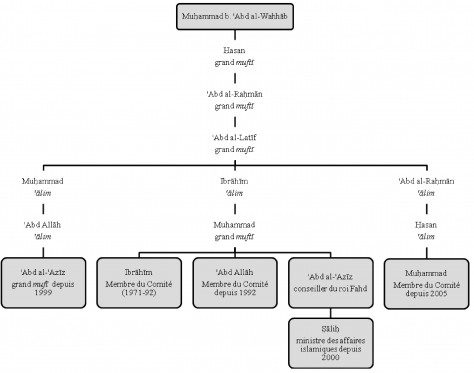
\includegraphics[width=\textwidth]{CourantsIslamContemporain/ImagesCourantsIslamContemporain/genealogie.jpeg}

13 Reste à signaler le cas particulier des oulémas originaires du Hijâz
et d'al-Aḥsā', provinces connues pour leur organisation hétéroclite. En
effet, la plupart des membres du Comité des grands oulémas, originaires
de ces régions, sont issus de ce qu'on a appelé des «dynasties»
d'oulémas, \emph{buyūtāt `ilm}, ou maisons de savoir comme ils aiment
eux-mêmes se faire appeler (à l'instar des familles d'oulémas dans les
autres pays arabes). Plus important encore est le fait que les familles
de ces oulémas appartiennent aux quatre écoles juridiques du sunnisme.
Si le facteur familial revêt une importance certaine, le paramètre de
l'origine tribale doit aussi être pris en compte.
\end{quote}

\hypertarget{la-pruxe9dominance-du-croissant-najdux12b}{%
\section{\texorpdfstring{La prédominance du croissant
\emph{najdī}}{La prédominance du croissant najdī}}\label{la-pruxe9dominance-du-croissant-najdux12b}}

\begin{quote}
14 Force est de constater que l'appartenance à une tribu, généralement
réinventée, constitue un critère identitaire important, dans une société
qui commence à peine à s'individualiser: avant d'être citoyen ou sujet,
on appartient d'abord à une tribu. C'est dire l'importance du milieu
tribal en tant que champ de socialisation des individus. La
\emph{`aṣabiyya}, l'esprit de corps tribal, joue un rôle fondamental
dans le statut social et la promotion de l'individu en Arabie Saoudite.

15 Les oulémas d'origine tribale dominent largement le Comité des grands
oulémas (il s'agit des tribus sédentarisées à partir du e siècle). Ils
sont quarante et un sur les cinquante-deux membres qu'a comptés le
Comité, depuis sa création, à être d'origine tribale, soit 79\%. Les
oulémas d'origine tribale se taillent ainsi la part du lion depuis 1971.
Les onze sièges restants sont occupés par des oulémas issus de trois
milieux différents: des membres de la notabilité citadine du Hijâz
(cooptés pour représenter les intérêts de leur région: on essaie de
choisir les plus «wahhabisés» et/ou quiétistes des oulémas du Hijâz),
des étrangers naturalisés (ils sont hanbalo-wahhabites, ont des talents
«exceptionnels» et ont défendu le hanbalo-wahhabisme et l'État) et des
citadins du Najd, sans affiliation tribale ou \emph{ḫaḍīrī}-s (ces
derniers ne doivent, en principe, leur ascension sociale qu'à leurs
compétences personnelles).

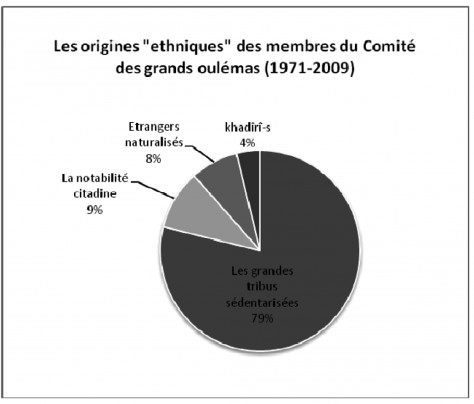
\includegraphics[width=4.9375in,height=4.20833in]{Image/media/image10.jpeg}

16 On constate alors, chiffres à l'appui, que l'appartenance au milieu
tribal sédentarisé joue un rôle déterminant dans l'ascension sociale des
oulémas, la \emph{`aṣabiyya} étant une valeur ajoutée qui permet de se
constituer un capital social. Cela dit, bien que les tribaux dominent
largement en nombre le Comité des grands oulémas, ils ne sont

toutefois pas représentatifs du paysage tribal saoudien. En effet,
certaines tribus comme les Banū Tamīm, les Banū Zayd et les Banū Ḫālid
sont «surreprésentées», tandis que d'autres comme les `Utayba n'ont
guère droit, malgré leur importance numérique, qu'à un seul représentant
au Comité des grands oulémas. D'autres tribus enfin, comme les Šammar,
les Ḥarb, les Muṭayr, les `Ajmān, les Ġāmid, etc. n'ont aucun
représentant au sein du Comité. Si la marginalisation des Šammar, des
`Utayba et des Muṭayr peut s'expliquer par leur passé de tribus
frondeuses, la marginalisation des autres tribus ne peut, elle, être due
qu'à des facteurs religieux et surtout régionaux. Nous nuancerons
seulement, pour finir, en précisant que, dans certains cas, le charisme
personnel du \emph{`ālim} -- c'est le cas d'Ibn Bāz -- fait «oublier»
son appartenance tribale. En effet, ce \emph{`ālim}, citadin sans
affiliation tribale, a pu grimper jusqu'au sommet de l'establishment
hanbalo-wahhabite (il devient grand mufti et président du Comité des
grands oulémas en 1993), uniquement grâce à son «érudition», à son
intégrité morale et à son dévouement aux Sa‛ūd. Le charisme et le
pouvoir symbolique d'Ibn Bāz ont fait de lui le plus grand \emph{`ālim}
hanbalo-wahhabite contemporain.

17 Le royaume d'Arabie Saoudite est un royaume \emph{najdī}. Les élites
saoudiennes sont majoritairement originaires de la région de Najd, fief
de la dynastie et de la doctrine hanbalo-wahhabite. Des études plus
récentes (datant de la dernière décennie) se fondent sur des données
chiffrées mais ne portent que sur les élites ministérielles, la haute
fonction publique et les membres du Conseil consultatif. Rien donc sur
les oulémas. Nous tenterons, dans ce qui suit, de combler ce manque. Sur
les cinquante- deux membres du Comité depuis sa création en 1971, 73\%
des oulémas sont originaires du Najd; 9\% du Ḥijāz, 6\% du Sud, 4\% de
la région orientale et 7\% d'origine étrangère.

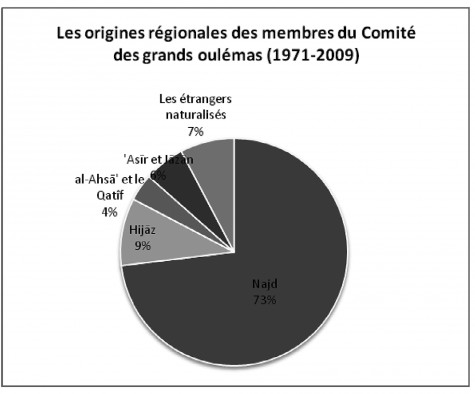
\includegraphics[width=4.94996in,height=4.10417in]{Image/media/image11.jpeg}

18 Une majorité des membres du Comité des grands oulémas est donc
\emph{najdī} et ce depuis sa création. Deux remarques pourraient être
faites à ce propos. La première est que si l'on peut aisément comprendre
que seuls 4\% des grands oulémas sont des Aḥsā'ī-s puisque une grande
partie de la population de cette province est chiite ou sunnite autres
que hanbalo-wahhabite; si l'on peut aussi comprendre que seuls 9\% des
grands oulémas sont \emph{ḥijāzī} puisque, bien que sunnites, ils ne
sont, généralement, pas hanbalo- wahhabites, le chiffre de 6\% seulement
d'oulémas originaires du Sud de l'Arabie Saoudite peut, du moins \emph{a
priori}, paraître absurde puisque les habitants de cette région sont en
majorité hanbalo-wahhabites. L'hypothèse de la préférence régionale peut
être ainsi raisonnablement soutenue: si 73\% des grands oulémas sont
\emph{najdī}, c'est, justement, parce qu'ils sont originaires du fief du
hanbalo-wahhabisme et de la maison
des Sa‛ūd et que, de ce fait, leur soumission à l'un et à l'autre ne
peut être remise en cause. La seconde remarque est que si l'on compare
les chiffres avancés pour le Comité des grands oulémas à ceux que
présente le conseil des ministres au sein duquel les Najdī constituent
72\% des membres (Ibn Ṣunaytān, 2004: 70-73); à ceux du Conseil
consultatif où les Najdī sont majoritaires à 51\% (\emph{ibid}.: 93-96);
à ceux des ministres plénipotentiaires qui sont à 78\% originaires du
Najd ou encore, à ceux des hauts fonctionnaires qui comptent 67\% de
Najdī (\emph{ibid}.: 177-178), on voit que l'élite saoudienne étatique,
qu'elle soit religieuse ou politique, est majoritairement \emph{najdī}.
Les gens du Sud, eux, qui, comme on l'a dit, sont majoritairement
hanbalo-wahhabites, ne représentent que 1\% des ministres, 7\% des
membres de Conseil consultatif, moins de 5\% des ministres
plénipotentiaires et moins de 9\% des hauts fonctionnaires
(\emph{ibid}.: 177- 178): le même raisonnement peut être, ici,
développé. Le régionalisme primerait en Arabie Saoudite. Même si l'on
parle de saoudisation et de formalisation, l'État continue toujours de
s'appuyer sur l'élément najdo-wahhabite pour fonctionner.

19 Observons les chiffres de plus près: lorsque 9\% seulement des
oulémas sont originaires du Hijâz, 20\% des membres du conseil des
ministres, 29\% des membres du Conseil consultatif, 22\% des hauts
fonctionnaires sont \emph{ḥijāzī} (et 34\% parmi eux des cadres
supérieurs). Par ailleurs, en observant les chiffres de plus près
encore, il apparaît qu'au moment de la création du Comité, 29\% des
oulémas sont originaires du Hijâz contre 9\%, nous l'avons dit,
aujourd'hui. Le Comité tend donc, au fur et à mesure qu'il se met en
place et qu'il n'a plus besoin de cadres supérieurs, à se fermer à tout
ce qui n'est pas \emph{najdī}. Il faut ajouter à cela que les oulémas,
quand ils ne sont pas hanbalo- wahhabites, dissimulent leurs croyances
-- ou du moins évitent d'en parler -- et ne jouent, une fois admis au
sein du Comité, qu'un rôle de «figurants».

20 Le Comité des grands oulémas voudrait donner une illusion
d'ouverture: les principales régions sont toutes, même à une faible
proportion, «représentées». Actuellement, deux oulémas d'origine
\emph{ḥijāzi}, deux oulémas originaires du Sud et un autre de l'Est sont
membres du Comité des grands oulémas. En réalité, l'élément \emph{najdī}
domine toujours le Comité, et de loin; de plus, en supposant qu'il y ait
ouverture et même si le Comité accepte en son sein des chiites, il lui
suffirait de conserver une majorité de 51\% de hanbalo-wahhabites
(Najdī) pour que le vote à la majorité absolue passe au sein du Comité
et qu'ainsi, la vision hanbalo-wahhabite continue à dominer.

21 Enfin, en ce qui concerne les oulémas d'origine étrangère, ils ne
sont admis au sein du Comité (au nombre de trois) qu'au moment de la
création de ce Comité. Ces oulémas étrangers étaient, en effet, plus
compétents et plus qualifiés que les oulémas locaux; ils étaient dévoués
à l'État et au hanbalo-wahhabisme; nés non-wahhabites, ils l'étaient
devenus par conviction; ils n'avaient pas d'assise sociale et tribale en
Arabie Saoudite et devaient leur ascension à l'État; enfin, la
solidarité islamique, initiée par le roi Fayçal, entrait également en
ligne de compte. Depuis, le Comité s'est fermé aux étrangers et même les
enfants des dits oulémas étrangers ne sont pas admis au sein du Comité.

22 Le tracé reliant les villes du Najd dont les grands oulémas sont
originaires forme,
pour ainsi dire, un croissant que nous conviendrons d'appeler «croissant
\emph{najdī}» et qui constitue l'épicentre de l'Arabie Saoudite en même
temps que celui du hanbalo- wahhabisme. Il ne faut toutefois pas croire
que si les oulémas du Najd sont largement majoritaires au sein du
Comité, toutes les villes et les régions du Najd y seront équitablement
«représentées». Le Najd compte trois principales régions: la région de
Riyad qui a donné vingt-sept oulémas, le Qaṣīm dix et le Ḥā'il qui n'a
donné aucun \emph{`ālim}. Les deux régions, de Riyad et du Qaṣīm,
offrent un quasi-équilibre dans la répartition des oulémas: dans la
région de Riyad, en dehors de la ville elle-même, qui donne, à elle
seule, sept oulémas, les autres villes donnent, chacune, entre un et
quatre oulémas. De même, dans la région du Qaṣīm, le nombre d'oulémas
par ville varie entre un et trois.

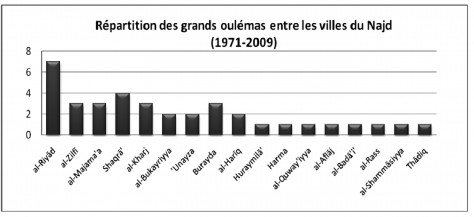
\includegraphics[width=4.9375in,height=2.26042in]{Image/media/image12.jpeg}

23 Le Ḥā'il, quant à lui, est volontairement marginalisé pour une raison
historique évidente: l'émirat du Ḥā'il a longtemps été le rival direct
des Saoud. Nous retrouvons à peine un représentant de cette région dans
le conseil des ministres et un seul autre au Conseil consultatif (Ibn
Ṣunaytān, 2004: 71 et 94).

24 Notons, pour finir, que certaines régions du Najd sont totalement
exclues et n'ont donné aucun \emph{`ālim}: l'exemple d'al-Dawādimī, pour
ne citer que lui, explique ce phénomène dans la mesure où la plupart des
habitants de la ville sont issus de la tribu des `Utayba dont la
fidélité au régime est douteuse. Il y aurait ainsi sous-régionalisation
à l'intérieur même de la régionalisation. De même, aucun grand
\emph{`ālim} n'est issu des régions du Nord. Enfin, aucun chiite n'est
admis au Comité des grands oulémas et ce, pour des raisons évidentes
qu'il ne semble pas utile de rappeler ici. Cela dit, les acquis familial
et tribal, seuls, ne suffisent pas: l'apprenti grand \emph{`ālim} doit
encore suivre un cursus d'études particulier pour intégrer le Comité.
\end{quote}

\hypertarget{de-la-ijux101za-au-doctorat-institutionnalisation-de-la-formation-du-ux101lim}{%
\section{\texorpdfstring{De la \emph{ijāza} au doctorat,
institutionnalisation de la formation du
‛ālim}{De la ijāza au doctorat, institutionnalisation de la formation du ‛ālim}}\label{de-la-ijux101za-au-doctorat-institutionnalisation-de-la-formation-du-ux101lim}}

\begin{quote}
25 Sur les cinquante-deux oulémas qui ont été membres du Comité des
grands oulémas depuis sa création, en 1971, 22\% (soit treize oulémas)
ont reçu une formation traditionnelle et 78\% (soit trente-neuf oulémas)
une formation «moderne». Près d'un quart des oulémas sont ainsi passés
par un cursus traditionnel. Nos entretiens nous permettent de décrire ce
\emph{ta‛līm} et d'en ressortir avec le cursus traditionnel «idéal
typique» du \emph{`ālim} hanbalo-wahhabite.

26 Au départ, entre l'âge de cinq et sept ans, l'apprenti \emph{`ālim}
fait son apprentissage du Coran. Les apprentis oulémas issus d'un milieu
modeste, ceux qui seront plus tard des self-made-men, apprennent le
Coran dans une école coranique (\emph{al-kuttāb}), aux mains d'un cheikh
de renommée moyenne. Les enfants des «cadres religieux moyens» et les
rejetons des dynasties d'oulémas, eux, apprennent le Coran auprès de
leur père, de l'un des membres de leur famille, ou d'un précepteur. On
imagine bien les difficultés rencontrées par les apprentis grands
oulémas issus de milieux modestes et le décalage qui se marque, dès le
départ, entre les apprentis oulémas issus des différentes classes
sociales.

27 Après cette phase d'apprentissage du Coran, l'apprenti \emph{`ālim}
doit, d'une part, commencer à étudier la grammaire et la rhétorique
arabes, de l'autre, apprendre par cœur les trois principaux ouvrages
d'Ibn `Abd al-Wahhāb sur l'unicité divine (\emph{al- tawḥīd}),
fondements du hanbalo-wahhabisme.

28 La troisième étape du cursus classique de l'apprenti \emph{`ālim} est
la quête du savoir
auprès des oulémas réputés. Le futur grand `ālim doit, en effet, réunir
un grand nombre de \emph{ijāzāt} (pl. de \emph{ijāza}: licences), dans
toutes les branches du savoir islamique disponibles, notamment en droit
et en théologie. Il assiste, pour ce faire, plus ou moins
assidûment, à des \emph{ḥalaqāt} `\emph{ilmiyya} ou cercles de savoir,
organisés quotidiennement dans les mosquées ou aux domiciles des
oulémas. Il s'agit alors, de séances de lectures mécaniques suivies de
commentaires d'ouvrages de hadith, d'exégèse coranique, de droit et de
théologie, notamment l'étude des œuvres classiques hanbalites. C'est à
l'issue de ces \emph{ḥalaqāt}, et une fois que l'étudiant a bien retenu
l'ensemble de l'enseignement dispensé par le \emph{`ālim}, qu'il fait un
\emph{istid`ā'}: une demande d'\emph{ijāza} pour les ouvrages étudiés.
Les étudiants les plus brillants deviennent assistants du maître et cela
leur ouvre la porte pour devenir professeur ou juge: la carrière est
alors lancée. Cela a été le cas de Muḥammad al-Sbayyil, le dernier grand
\emph{`ālim} à avoir reçu une formation traditionnelle.

29 Né dans la région du Qaṣīm vers 1926, al-Sbayyil est issu d'une
famille de «cadres religieux moyens». Son père, libraire et copiste
d'ouvrages religieux, connaît parfaitement le Coran. Son frère aîné,
`Abd al-`Azīz, est un \emph{`ālim} de la ville d'al- Bukayriyya. À l'âge
de cinq ans, al-Sbayyil commence son apprentissage du Coran auprès de
son père puis de son frère. Vers l'âge de dix ans, il se lance dans
l'apprentissage des trois ouvrages fondamentaux d'Ibn `Abd al-Wahhāb. Il
étudie aussi la jurisprudence hanbalite sous la direction des oulémas du
Qaṣīm, notamment les ouvrages d'Ibn Taymiyya (m. 1328), d'Ibn Qayyim
al-Jawziyya (m. 1350) et de Mar`ī al- Karamī (m. 1624), etc. À l'âge de
vingt ans, il aurait déjà acquis plusieurs \emph{ijāzāt} qui lui
permirent de devenir l'assistant du juge du Qaṣīm, `Abd Allāh b. Ḥumayd.

30 La formation traditionnelle indispensable au tout début du e siècle
perd, peu à peu, du terrain. En effet, les oulémas qui ont reçu cette
formation s'adaptent difficilement aux exigences de la modernité. 53\%
des membres du Comité des grands oulémas, soit neuf oulémas, ont reçu,
en 1971, une formation dite traditionnelle; en 2009, aucun grand
\emph{`ālim} ne bénéficie d'une telle formation. Dans un pays qui tente
de se moderniser, le besoin d'uniformisation de la formation des grands
oulémas s'impose. Il a fallu, pour y répondre, créer un cursus complet,
homogène, un cursus «national». Nous entendons par cursus moderne, un
cursus «institutionnalisé» et uniformisé.

31 S'ils ne sont que 47\% (soit huit oulémas), en 1971, à suivre la
formation dite moderne,

ils sont aujourd'hui 100\% à le faire. Après un cycle d'études primaires
dans des écoles publiques2\emph{,} les élèves qui se destinent à faire
une carrière juridico-religieuse, rejoignent les instituts de sciences
religieuses (\emph{al-ma`āhid al-`ilmiyya}). Le premier institut voit le
jour à Riyad, en 1950, à l'instigation du grand mufti du royaume de
l'époque, Muḥammad b. Ibrāhīm. Mais très vite, le gouvernement adopte le
projet et les instituts fleurissent dans toutes les régions du royaume
pour atteindre le chiffre de soixante- deux en 2009. Pour accéder à
l'enseignement de ces instituts, l'enfant doit avoir un dossier correct
et avoir appris au moins deux parties du Coran. L'enseignement y est
gratuit. Les instituts de sciences religieuses proposent un cursus de
six années: trois années de collège sanctionnées par un certificat de
réussite, sorte de «brevet» et trois années de lycée sanctionnées par un
certificat de réussite, sorte de «baccalauréat». Les matières étudiées
ont évolué depuis les années cinquante. Au début, l'enseignement était
constitué de quatre troncs communs: les sciences religieuses, les
sciences de la langue arabe, les «sciences sociales», et les
mathématiques. Au fil des années, on a ajouté à ce tronc commun d'études
de base, l'apprentissage obligatoire de la langue anglaise et de
l'informatique. Ces instituts de sciences religieuses sont inégalement
répartis sur l'ensemble du pays: le Najd compte 34\% des instituts, le
Hijâz 13\%, le Sud 28\%, le Nord 18\%, l'Est, enfin, 7\%. Les instituts
sont nombreux dans les régions où le hanbalo-wahhabisme est majoritaire
c'est-à-dire dans le Najd, le Sud et le Nord.

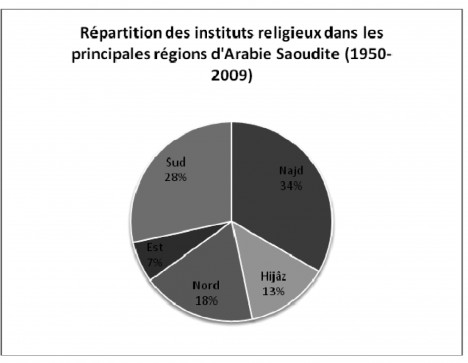
\includegraphics[width=4.875in,height=3.78125in]{Image/media/image13.jpeg}

32 Si la proportion entre le nombre d'instituts créés dans le Hijâz et
celui des oulémas qui sont admis au Comité des grands oulémas est
relativement équilibrée, la proportion entre le nombre d'instituts créés
dans les trois autres régions hanbalo-wahhabites et celui des oulémas
issus de ces régions et effectivement admis au sein du Comité, est,
quant à elle, largement déséquilibrée. On s'attendrait, en effet, à un
nombre plus important d'instituts de sciences religieuses dans le Najd,
à un nombre moins important dans le Sud et à un nombre nul d'instituts
dans la région du Nord. Or, ils sont créés dans le Nord et dans le Sud
mais ce, moins dans le but de former des grands oulémas que dans celui
de «wahhabiser» ces régions en y formant des techniciens du culte
hanbalo-wahhabite et des «cadres religieux moyens».

33 Lorsque l'apprenti \emph{`ālim} a terminé avec succès ses études
secondaires au sein de l'institut, il peut postuler pour les trois
grandes universités du pays: l'Université islamique de Médine (al-Jāmi`a
al-islāmiyya), l'Université islamique de la Mecque (Jāmi`at Umm al-Qurā)
et l'Université islamique de Riyad (Jāmi`at al-imām Muḥammad b. Sa`ūd
al-islāmiyya).

34 La première de ces universités, fondée en 1961, accueille surtout les
musulmans étrangers. Les Saoudiens qui y étudient se destinent
généralement à la prédication à l'étranger. De cette université n'est
issu qu'un seul grand \emph{`ālim}.

35 Quant à la deuxième citée, elle est la plus ancienne université de
théologie d'Arabie Saoudite, fondée en 1949. Elle n'a, malgré son
ancienneté, donnée que six grands oulémas. Doit-on y voir une
manifestation du régionalisme saoudien? Toujours est-il que cette
université accueille, depuis les années soixante-dix, des professeurs,
des cadres et des étudiants de diverses tendances politico-religieuses,
notamment des frères musulmans et des sahwistes (Lacroix, 2010: 47-97)
en lesquels le gouvernement saoudien et le Comité des grands oulémas
n'ont que très peu confiance et qui ne sont donc pas spontanément
recrutés par celui-ci.

36 La dernière université, enfin, est incontestablement la plus
importante pour notre étude. Elle a donné vingt-cinq oulémas, soit 51\%
des membres du Comité, depuis sa création en 1971, et 75\% des oulémas
ayant fait des études universitaires modernes. Cette université naît, en
1974, de la fusion de la faculté de théologie créée, elle, en 1953, et
de la faculté de langue arabe, créée en 1954.

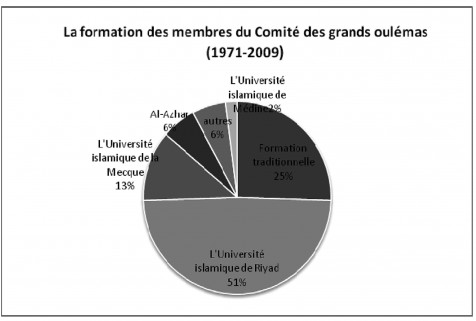
\includegraphics[width=4.95833in,height=3.34375in]{Image/media/image14.jpeg}

37 Depuis sa création, l'Université islamique de Riyad, qui,
rappelons-le, porte le nom du fondateur de l'émirat saoudien Muḥammad b.
Sa`ūd (1744-1765), fidèle allié d'Ibn `Abd al-Wahhāb, est considérée
comme le vivier des grands oulémas et de tous les cadres religieux et
techniciens du culte dont l'establishment religieux a besoin. Le

«pharaonique» campus de l'université (une véritable ville dans la ville
avec ses propres infrastructures, un petit hôpital, un supermarché, des
quartiers résidentiels pour les étudiants, les professeurs et le
personnel administratif, etc.) compte neuf facultés et deux instituts
supérieurs: la faculté de droit {[}musulman{]}; la faculté de théologie;
la faculté de langue arabe; la faculté des sciences sociales
{[}islamiques{]}; la faculté de la prédication et de la communication;
la faculté des langues et de la traduction; la faculté des sciences de
l'informatique; la faculté de l'économie; la faculté des sciences;
l'Institut supérieur de la magistrature et l'Institut de l'apprentissage
de la langue arabe {[}pour les étrangers{]}. Cela dit, les grands
oulémas sont exclusivement issus des facultés de droit et de théologie
et de l'Institut supérieur de la magistrature. Les étudiants dans ces
trois domaines bénéficient d'une bourse d'études et obtiennent, dès la
fin de leur première année d'études, le titre fort apprécié de
\emph{shaykh}. Le succès de l'Université islamique de Riyad est tel que
celle-ci s'est engagée dans une politique d'expansion en développant
deux filiales en Arabie Saoudite3 et cinq à l'étranger4\emph{.} Enfin,
certains étudiants peuvent préparer leur doctorat en sciences
religieuses à l'université égyptienne d'al-Azhar, pour le prestige que
cela donne. Une autre raison pourrait être avancée: certains apprentis
oulémas saoudiens iraient à al-Azhar pour observer l'organisation, les
structures et les mécanismes de fonctionnement de cette prestigieuse
université en vue de les
«importer» en Arabie Saoudite.

38 Les oulémas, au moment de leurs études supérieures, ont tous un tronc
commun tripartite: les fondements de la théologie (\emph{al-`aqīda});
l'exégèse coranique (\emph{al tafsīr}) et la jurisprudence
(\emph{al-fiqh}). À partir de la première année de master (calqué sur le
système anglo-saxon), 74\% des oulémas se spécialisent dans la
jurisprudence, et plus spécialement dans les fondements de la
jurisprudence islamique (\emph{uṣūl al-fiqh}) dans le but d'acquérir la
qualification requise pour émettre des \emph{fatwā}; 26\% d'entre eux,
se spécialisent en théologie, et plus précisément en religions comparées
(en réalité, pour dénigrer toute autre religion que l'islam
hanbalo-wahhabite)5\emph{.} Le choix de ces spécialisations n'est pas
étonnant dans la mesure où les étudiants se destinent avant tout à être
des techniciens du culte et des gestionnaires des biens de salut. Nous
n'entrerons pas, pour ne pas alourdir notre propos, dans le détail des
spécialisations pointues à l'intérieur même des deux grands domaines de
spécialisations que nous avons évoqués.

39 Bien que le cursus moderne se soit bien implanté dans le paysage
saoudien, l'ijāza
n'en demeure pas moins source de prestige et un élément non négligeable
dans un
capital social. Nous avons pu observer que la totalité des oulémas qui
ont suivi le cursus moderne ont, néanmoins, obtenu une ou plusieurs
\emph{ijāzāt}. Elément de prestige comme nous venons de le dire,
l'\emph{ijāza} est, en théorie, facultative. Mais, en pratique,
l'obtention d'une \emph{ijāza} permet au \emph{`ālim}, d'une part, de se
rattacher à une chaîne de transmission
«ininterrompue» d'oulémas remontant jusqu'au Prophète, ce qui permet au
\emph{`ālim} de légitimer sa position et son savoir et de s'inscrire
dans l'héritage prophétique, d'autre part, de nouer des relations
privilégiées avec un ou plusieurs oulémas et de commencer ainsi à tisser
un réseau qui pourra le mener au sommet de l'establishment hanbalo-
wahhabite.

\textbf{Faire carrière: le \emph{cursus honorum} des oulémas}

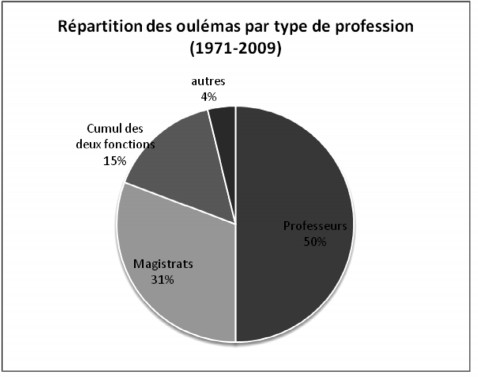
\includegraphics[width=4.97917in,height=3.92708in]{Image/media/image15.jpeg}40
L'enseignement et la magistrature ont toujours été les métiers de
prédilection des oulémas. Les membres du Comité des grands oulémas
n'échappent pas à cette règle. 96\% d'entre eux exercent au moins une de
ces deux professions: 50\% du Comité, soit vingt et un grands oulémas,
ont été ou sont encore, professeurs de jurisprudence islamique ou de
théologie; 31\% d'entre eux sont magistrats dans les différentes
instances de la justice saoudienne; 15\% des grands oulémas ont cumulé
les deux fonctions. À la question: «pourquoi le choix de ces métiers?»
Une première réponse, unanime, des grands oulémas magistrats: «la
justice est le fondement de la royauté». Et, selon les oulémas, qui,
mieux que des spécialistes de «la loi divine», pourraient mettre la
justice en application! Les grands oulémas ont d'ailleurs pleine
conscience de l'importance de leur mission. Ils ont une vision
catastrophiste d'un monde où le \emph{`ilm}, qui risque d'être perdu,
doit être sauvé, épuré des innovations blâmables et transmis par le
\emph{`ālim}.

41 En outre, si la magistrature permet au grand \emph{`ālim} d'observer,
d'analyser et de statuer sur des cas concrets, l'enseignement permet de
transmettre le savoir théorique. Cela, en plus du prestige qui entoure
ces deux fonctions. Il n'est, enfin, pas étonnant de voir que nombre de
grands oulémas cumulent les deux fonctions puisqu'en réalité, l'une et
l'autre sont indissociables (pratique et théorie). Ce phénomène de cumul
des fonctions (d'enseignant et de magistrat) est surtout visible dans la
première génération des grands oulémas. Il s'explique par le manque de
cadres religieux au moment de la
création du Comité. Les grands oulémas devaient donc assumer, tout à la
fois, leur rôle au sein du Comité et les fonctions de magistrats et
d'enseignants. Des années quarante aux années soixante, l'Arabie
Saoudite a été obligée d'«importer» des cadres religieux de l'étranger,
notamment de l'Égypte. Un exemple: l'Égyptien `Abd al-Razzāq `Afīfī (m.
1994), arrivé en Arabie Saoudite, en 1949, pour enseigner la langue
arabe et les sciences religieuses dans un collège à Tayef, a gravi, un à
un, les échelons et parvient au sommet de l'establishment religieux: il
est nommé, en 1971, au sein du Comité des grands oulémas. Cet exemple
révèle deux réalités: premièrement, l'Arabie Saoudite a fait appel aux
étrangers pour l'enseignement, à une certaine époque, à cause du déficit
de cadres dont elle a souffert dans tous les domaines; et deuxièmement,
les étrangers hanbalo-wahhabites, qui pouvaient aisément s'intégrer dans
le pays d'accueil, ont pu, à force de persévérance, atteindre le sommet
de l'establishment religieux saoudien.

42 La pratique du cumul des fonctions d'enseignant et de magistrat tend
à disparaître: le dernier grand \emph{`ālim} à avoir cumulé ces deux
fonctions est `Abd Allāh b. Qa`ūd, membre du Comité de 1977 à
19866\emph{.} Désormais, les grands oulémas, qu'ils soient professeurs
ou magistrats, sont de plus en plus spécialisés, chacun dans son
domaine: de professeurs de droit en général, ils sont devenus
professeurs de droit pénal, de droit de la famille, etc. Parallèlement à
ces deux métiers de prédilection, les grands oulémas sont techniciens du
culte: la plupart d'entre eux sont imâm dans les mosquées. Par exemple,
le grand mufti actuel du royaume, `Abd al-`Azīz āl al-Shaykh, est
également imâm de la grande mosquée de Riyad. Sāliḥ b. Ḥumayd est, lui,
imâm de la grande mosquée de la Mecque, etc. N'oublions pas enfin,
l'autre fonction essentielle des grands oulémas, celle d'«entrepreneurs»
de biens de salut, à savoir promulguer des \emph{fatwā} et se mettre à
l'écoute de la population. Mais si les grands oulémas monopolisent les
grands postes religieux et judiciaires saoudiens, ils n'hésitent pas à
empiéter sur le domaine réservé des autres élites.

43 Une fois admis au sein du Comité, le grand \emph{`ālim} obtient
automatiquement le grade de haut fonctionnaire (\emph{al-martaba
al-mumtāza}), voire celui de ministre. Sur les cinquante-deux membres du
Comité des grands oulémas, vingt-deux ont occupé des postes de
responsabilité autres que ceux de magistrats et d'enseignants. Déjà neuf
membres de la \emph{Hay'a} ont été ou sont encore ministres. Les
ministères que contrôlent les oulémas (si ce ne sont pas eux qui les
contrôlent directement, c'est un membre de l'establishment religieux)
sont ceux de la justice, des affaires islamiques, du pèlerinage et de
l'enseignement des filles (avant le rattachement de ce dernier, en 2002,
au ministère de l'éducation nationale). Depuis sa création, le ministère
de la justice est dirigé par un membre du Comité7\emph{.} Huit membres
du Comité des grands oulémas on été membres du Conseil consultatif: le
président de ce conseil, qui fait se côtoyer islamistes,
«libéraux», conservateurs et tribaux, depuis sa création, en 1992, est
un membre du Comité des grands oulémas. De 1992 à 2002, c'est Muḥammad
b. Jubayr, membre du Comité des grands oulémas (de 1971 à 2002), qui
assure la présidence de cette instance. Sāliḥ b. Ḥumayd, membre du
Comité des grands oulémas depuis 2001, lui succède en 2002. Ce dernier
est remplacé par `Abd Allāh Āl al-Shaykh, en 2009. Trois membres de la
\emph{Hay'a} ont été conseillers du roi Fahd (1982-2005) et deux sont
actuellement conseillers du roi `Abd Allāh. Quatre membres du Comité ont
occupé les postes de doyen ou de président d'université. Par exemple,
`Abd al-`Azīz b. Bāz occupe jusqu'à sa mort, en 1999, le poste de
président de l'Université islamique de Médine. Sa`d al- Ḍuwayḥī est
doyen de la faculté de théologie d'al-Aḥsā'. `Abd Allāh b. `Abd
al-Muḥsin al- Turkī, sans doute l'un des membres les plus actifs du
Comité, actuellement, occupe le poste de président de la Ligue islamique
mondiale, après avoir occupé, entre autres, les postes de président de
l'Université de Riyad et de ministre des affaires islamiques.

44 C'est dire que les oulémas ont adopté, depuis au moins deux
décennies, une stratégie adaptative qui les pousse à investir plusieurs
secteurs d'activités. Outre les domaines religieux, législatif et
éducatif, ils investissent les associations caritatives, les
organisations gouvernementales et non gouvernementales et les domaines
économique et financier. Dans ces deux derniers domaines, trois oulémas,
`Abd Allāh b. Manī`, `Abd
al-Wahhāb Abu Sulaymān et `Abd Allāh al-Muṭlaq se sont «improvisés»
experts et consultants incontournables dans les marchés financiers
saoudiens. Les trois hommes sont aussi membres de plusieurs conseils
d'administration de banques et d'entreprises dans le cadre de ce que
l'on appelle en Arabie Saoudite \emph{al-lijān al-šar`iyya} ou
commissions islamiques. Le nom-même d'un grand \emph{`ālim} sur la
brochure d'une société ou d'une entreprise est la meilleure des
publicités.
\end{quote}

\hypertarget{la-multiplication-des-ruxe9seaux-de-soutien}{%
\section{La multiplication des réseaux de
soutien}\label{la-multiplication-des-ruxe9seaux-de-soutien}}

\begin{quote}
45 Cette mobilité des oulémas n'est, toutefois, possible que si le
\emph{`ālim} tisse, autour de lui, un réseau sur lequel il peut
s'appuyer. Les capitaux culturel et économique doivent encore être
complétés par un réseau de soutiens. Nous avons pu observer trois types
de capitaux sociaux mobilisés par le futur grand \emph{`ālim}. Autrement
dit, le recours aux relations personnelles permet à ce dernier de
s'assurer une meilleure position dans la hiérarchie sociale. Ces trois
réseaux, que nous exposons séparément, sont en réalité, presque
toujours, combinés par le futur grand \emph{`ālim}. Le réseau familial
constitue la première ressource du futur grand \emph{`ālim}. Nous avons,
en effet, constaté l'existence d'au moins trois exemples de réseaux
familiaux qui sont autant de moyens d'accès au Comité des grands
oulémas.

46 Le premier est, sans aucun doute, le plus puissant et le plus dense:
celui des Āl al- Shaykh. Nous avons évoqué plus haut l'importance de
cette famille et nous tenterons, dans ce qui suit, de compléter le
tableau amorcé. L'exemple des deux fils, Ibrāhīm et `Abd Allāh, du grand
mufti Muḥammad b. Ibrāhīm est tout à fait significatif: bien que le
premier des deux ait été relativement peu brillant par rapport aux
collaborateurs de son père, il a quand même été nommé par ce dernier
vice-mufti du royaume d'Arabie Saoudite. Après la mort de son père et la
suppression du poste de mufti, Ibrāhīm, qui était destiné à devenir
mufti, reçoit, en guise de consolation, les postes de ministre de la
justice, de membre du Comité des grands oulémas et de président de la
Direction de la recherche scientifique, de la prédication et de
l'instruction! En 1992, lorsqu'Ibrāhīm se retire des affaires, son
remplaçant au ministère et au Comité des grands oulémas n'est autre que
son frère cadet `Abd Allāh, président actuel du Conseil consultatif. Un
autre exemple étonnant de la famille Āl al-Shaykh: il s'agit de Ṣāliḥ b.
'Abd al-`Azīz, le petit fils d'Ibn Ibrāhīm. Après avoir fait des études
scientifiques depuis le lycée et obtenu un diplôme d'ingénieur, Ṣāliḥ
décide de récupérer l'héritage familial et s'inscrit à l'Université
islamique de Riyad. Grâce à son nom et à l'intervention de son père, qui
était l'un des conseillers du roi Fahd, il obtient une équivalence et
passe ainsi directement en année de master: il contourne la règle qui,
aussi stricte soit-elle, s'efface quand il s'agit d'un Āl al-Shaykh. Il
est actuellement ministre des affaires islamiques et, potentiellement,
membre du Comité des grands oulémas. Un dernier exemple enfin de cette
famille: le dernier admis à Hay'at kibār al-'ulamā', Muḥammad b. Ḥasan,
fait une ascension fulgurante grâce à ses bonnes relations avec son
cousin, le grand mufti actuel d'Arabie Saoudite: il a pu, rapidement,
gravir les échelons universitaires et devenir le directeur de cabinet du
mufti. Ce dernier l'épaule et le soutient: il propose son nom au Comité
des grands oulémas auquel Muḥammad b. Ḥasan accède en avril 2005.
Signalons, enfin, que le réseau familial des Āl al-Shaykh et l'influence
qui en découle, dépassent largement le seul cadre religieux: un membre
de la famille est ambassadeur à Paris, un autre est directeur du
protocole royal, un troisième est membre de la chambre de commerce, etc.
Le deuxième réseau familial est celui des Ibn Ḥumayd, déjà présenté plus
haut.

47 Le dernier réseau familial, enfin, de moindre importance, est celui
des al-Šathrī: cette
famille du Najd a donné quelques oulémas et plusieurs hommes politiques.
`Abd al-‛Azīz al-Šathrī, un des conseillers des rois Fayçal (1964-75) et
Ḫālid (1975-82) a également été un ouléma de renommée moyenne. Son fils,
Nāṣir, a réussi à faire une brillante carrière politique (en tant que
conseiller des rois Ḫālid et Fahd). Selon un des
membres du clan al-Šathrī: «il ne manquait à {[}la{]} famille qu'un
grand \emph{`ālim} pour qu'{[}elle{]} devienne, enfin, une grande
famille». La parentèle met tout en œuvre pour que son rejeton prodige,
Sa‛d, accède au sommet de l'establishment religieux. Aussi, le
prépare-t-on, dès son plus jeune âge, à devenir grand \emph{`ālim} : on
le confie aux maîtres les plus compétents dans le domaine, tels Ibn Bāz,
Ibn `Uthaymīn, al-Aṭram, al-Rakbān et `Abd al-`Azīz Āl al-Shaykh. On le
pousse à s'inscrire à Jāmi'at al-imām où il obtient un doctorat en
fondements de la jurisprudence islamique. Sa`d brûle toutes les étapes
du \emph{cursus honorum} hanbalo-wahhabite et devient professeur de la
même université en un temps records. En mars 2005, la famille soutient
la candidature de son fils au Comité des grands oulémas (le père est
membre du cabinet royal qui transmet les candidatures au roi). Sa`d est
finalement nommé, en avril 2005: à trente-huit ans, il est le plus jeune
membre de l'histoire du Comité des grands oulémas.

48 Nous l'avons dit, le régionalisme et le segmentarisme dominent le
paysage politico- religieux saoudien. La deuxième ressource du futur
grand \emph{`ālim} est, naturellement, le réseau tribal qui va de pair
avec le réseau régional, autrement dit avec le réseau \emph{najdī}. Nous
avons remarqué, en analysant les origines géographiques et tribales des
grands oulémas, que ces derniers sont généralement issus des plus
grandes confédérations tribales du Najd: les Banū Ḫālid ont donné quatre
grands oulémas, les Banū Zayd, sept, les Banū Subay`, trois, les Banū
Tamīm, huit (auxquels il faut ajouter les quatre grands oulémas des Āl
al-Shaykh), les Qaḥṭān, trois, les `Unayza, trois, les Bāhila, deux et
al- Dawāsir, deux également. Soit un total de trente-six grands oulémas
issus des grandes tribus du Najd sur les cinquante-deux membres du
Comité. Le réseau tribal est très dense. Le nombre de grands oulémas est
plus ou moins bien réparti entre les grandes tribus \emph{najdī}. D'un
mouvement de nomination au sein du Comité à l'autre, cet équilibre est,
consciemment ou inconsciemment, maintenu. Exemple: les deux grands
oulémas, Muḥammad āl Sulaymān et Bakr Abū Zayd, de la tribu des Banū
Zayd -- admis tous deux au Comité, en 1992 -- sont remplacés, en 2005,
par deux hommes issus de la même tribu, `Alī al-Ḍuwayḥī et `Abd
al-Raḥmān al-Sadḥān. D'ailleurs, le réseau tribal doublé du réseau
régional ne concerne pas uniquement le champ religieux: on retrouve ces
mêmes configurations dans le domaine politico-administratif (Ibn
Ṣunaytān, 2004, 59-62).

49 La dernière ressource du futur grand \emph{`ālim} est la
\emph{mulāzama}: le fait de s'attacher un
long moment à un maître en sciences religieuses, réputé et influent.
Côtoyer un maître pendant plusieurs années permet à l'apprenti grand
\emph{`ālim} de nouer avec lui des relations personnelles qui peuvent
même aboutir au mariage de l'élève avec la fille ou la nièce du maître.
Par exemple, Ṣāliḥ al-Luḥaydān est, pendant plusieurs années, le
disciple favori du grand mufti Muḥammad b. Ibrāhīm. Cette relation
privilégiée lance véritablement la carrière de Ṣāliḥ qui devient le
gendre et le directeur de cabinet du mufti et qui gagne peu en peu en
charisme. Une année seulement après le décès du maître, al-Luḥaydān est
admis au Comité des grands oulémas; il hérite aussi de la fonction de
magistrat; quelques années plus tard, il devient le président du Haut
conseil de la magistrature, poste qu'il occupe jusqu'en février 2009.
Al-Luḥaydān est le doyen du Comité des grands oulémas dont il est membre
depuis 1971. Il en est aussi un des membres les plus influents. Il
serait, en effet, le seul à pouvoir opposer un veto pour la nomination
d'un nouveau membre: en 2005, il aurait utilisé son veto pour s'opposer
à l'entrée de l'ouléma `Abd al-Muḥsin al-`Ubaykān au Comité.

50 Un autre exemple: Muḥammad al-Sbayyil est le disciple d'Ibn Ḥumayd
alors que
celui-ci est le \emph{qāḍī} d'al-Bukayriyya. Quand Ibn Ḥumayd devient le
\emph{qāḍī} du Qaṣīm, il fait appeler al-Sbayyil à Burayda pour le
désigner professeur et responsable d'un institut de sciences religieuses
de la région. La relation entre les deux hommes est telle que,
lorsqu'Ibn Ḥumayd devient le grand juge du Ḥijāz, il le fait venir à la
Mecque et le nomme imâm de la grande mosquée de la Mecque et
vice-président de l'administration chargée de gérer les deux lieux
saints. Il finit même par en devenir président (jusqu'en 2005) après la
disparition de son protecteur. Depuis son arrivée à la Mecque, il tisse
des
relations étroites avec des oulémas et grands oulémas notamment Ibn Bāz
(qui n'est pas son maître) mais qui finit par lui proposer de devenir
membre du Comité en 1992.

51 Un troisième exemple: c'est également Ibn Bāz qui suit, pas à pas, la
carrière de `Abd
Allāh b. Qa'ūd qui est son meilleur disciple. À la première occasion (le
décès d'Ibn Ḥumayd et de Miḥḍār `Aqīl), Ibn Bāz propose le nom d'Ibn
Qa`ūd au cabinet royal qui le nomme membre du Comité en 1977.

52 Un dernier exemple enfin: le mufti actuel, `Abd al-`Azīz āl
al-Shaykh, en plus du réseau familial que lui confère son nom, bénéficie
du soutien de son maître Ibn Bāz. Il s'agit d'abord d'une question de
solidarité et de reconnaissance: Ibn Bāz est un \emph{mulāzim} du grand
père de `Abd al-`Azīz Āl al-Shaykh, Muḥammad b. `Abd al-Laṭīf. Il aide
donc `Abd al-`Azīz Āl al-Shaykh à devenir professeur à l'université
d'al-Imām, et propose son nom au cabinet royal pour en faire un membre
du Comité des grands oulémas (il le deviendra en 1987). En 1993, Ibn Bāz
devient mufti et désigne `Abd al-`Azīz āl al-Shaykh vice-mufti du
royaume et ce, bien que d'autres grands oulémas soient plus compétents
que lui. En effet, depuis les années soixante et jusqu'à sa mort, en
1999, Ibn Bāz occupe une position-clé dans l'establishment religieux. Il
bénéficie du respect et de la considération des autres grands oulémas et
exerce, de ce fait, une influence autour de lui, tous les grands oulémas
tenant compte de ses conseils et suivant à la lettre ses directives. La
centralité d'Ibn Bāz est ainsi très importante: un grand nombre de
chemins passent par lui. Dix-huit grands oulémas sont ses disciples et
certains d'entre eux lui doivent leur entrée au sein du Comité.
\end{quote}

\hypertarget{le-quiuxe9tisme-politique}{%
\section{Le quiétisme politique}\label{le-quiuxe9tisme-politique}}

\begin{quote}
53 En cherchant à identifier les conditions d'accès au Comité des grands
oulémas à travers le parcours de ses membres, nous avons constaté qu'il
existe deux critères directement liés à la vie politique et sociale:
aucun des grands oulémas n'a de passé politique (c'est-à-dire, une
quelconque manifestation d'opposition au régime: demande de réformes, ou
autres), et aucun \emph{`ālim} n'a jamais critiqué les décisions du
Comité ou de l'un de ses membres et ce, même si ses positions allaient à
l'encontre des décisions officielles.

54 `Abd Allāh Ibn Jibrīn, haut fonctionnaire religieux et candidat
potentiel au Comité des grands oulémas, a été l'un des parrains de la
contestation islamiste des débuts des années quatre-vingt-dix (Kepel,
2003: 335-337; Lacroix, 2007: 371-443). Ces actes constituent une
véritable offense tant pour le régime que pour les grands oulémas. Ces
derniers ne manquent pas, d'ailleurs, de le désavouer publiquement: il
est démis de ses fonctions officielles. Réhabilité par la suite, et bien
que très bon \emph{`ālim}, il ne pourra cependant jamais prétendre au
poste de grand \emph{`ālim} en raison de cette «bavure»: s'étant
ouvertement opposé au gouvernement et ayant participé à des activités
politiques allant à l'encontre des positions officielles, son «rachat»
et son récent soutien au gouvernement ne suffisent pas. Il ressort de
cet exemple que le quiétisme politique des candidats au Comité est un
élément fondamental et un critère-clé de sélection. Tout ce que peut
tolérer le Comité comme engagement politique pour un futur grand
\emph{`ālim} est le soutien aux décisions du pouvoir. `Alī al-Ḍuwayḥī
est l'exemple du \emph{`ālim} engagé politiquement -- en faveur du
régime bien sûr -- qui accède à la Hay'a. En effet, depuis 2001,
al-Ḍuwayḥī, qui dirige la faculté de théologie d'al-Aḥsā', a signé
plusieurs pétitions politiques défendant les programmes scolaires
saoudiens, et se déclarant en faveur de la tenue d'élections
municipales, etc.

55 Quant à `Abd al-Muḥsin al-`Ubaykān, qui a appelé ouvertement le
gouvernement à entreprendre des réformes, entre 1992 et 1994, il a été
marginalisé et démis de ses multiples fonctions: il perd son poste de
juge au tribunal de Riyad et d'imâm de mosquée. Réhabilité, dans les
années 1999-2000, il continue néanmoins à critiquer les décisions de la
Hay'a (surtout celles qui concernent la jurisprudence), et du système
judiciaire. Il émet même des \emph{fatwā} contredisant celles du Comité
des grands oulémas et
tente, pour se rattraper, de promulguer des \emph{fatwā} sur la licéité
du salut du drapeau national, sur la condamnation des sahwistes ou
encore sur l'interdiction du djihâd en Irak pour les Saoudiens. Le
gouvernement a accepté de le réhabiliter mais les oulémas ont opposé un
veto catégorique à l'entrée de ce \emph{`ālim} au Comité. Al-`Ubaykān a,
finalement, été nommé, dans un premier temps, conseiller au ministère de
la justice et membre du Conseil consultatif, avant de devenir l'un des
conseillers du roi, en 2009.

56 Les leaders de la \emph{ṣaḥwa} dans les années quatre-vingt-dix,
Safar al-Ḥawālī, Salmān al-`Awda et Muḥsin al-`Awājī, reconnaissent
eux-mêmes que l'un des critères d'accès au Comité des grands oulémas est
le quiétisme sur les plans politique et sécuritaire et acceptent donc,
du fait de leur très grand engagement politique, de ne pas y prétendre.

«Pour le gouvernement, dit al-Ḥawālī, les grands oulémas doivent être
des hommes apolitiques, des hommes qui ignorent tout de la politique».
Salmān al-`Awda ajoute que

«les futurs membres du Comité doivent être des hommes sans histoire(s)».
Pour Muḥsin al-`Awājī «l'accès au Comité obéit à des critères purement
sécuritaires».

57 Il découle de tout cela le «portrait idéal» du membre du Comité des
grands oulémas:

le grand \emph{`ālim} est hanbalo-wahhabite; il est issu d'une famille
de «cadres religieux moyens» ou d'une «dynastie» d'oulémas; il est issu
d'une grande tribu sédentarisée du croissant \emph{najdī}; il a effectué
des études auprès de maîtres réputés (cela pour le \emph{`ālim} qui suit
une formation traditionnelle) ou dans un \emph{ma`had `ilmī} puis à
l'université al-Imām de Riyad (pour le grand \emph{`ālim} qui a reçu une
formation moderne); il s'est spécialisé en jurisprudence islamique; il
est généralement professeur d'université (al-Imām) ou magistrat; il a en
moyenne vingt-cinq années d'expérience dans le domaine religieux; il
n'est pas engagé politiquement (s'il l'est, il ne doit l'être qu'en
faveur du régime).

58 La moyenne d'âge du grand \emph{`ālim} qui accède au Comité est de
quarante-sept ans. Il y reste en moyenne quinze ans. Et, si les
circonstances d'accès à la Hay'a sont difficiles à déterminer, les
circonstances de départ de la Hay'a sont, elles, tout à fait claires: le
grand \emph{`ālim} quitte le Comité s'il décède, bien évidemment, s'il
est gravement malade ou s'il a commis un acte jugé répréhensible par le
roi -- en 1992, quatre grands oulémas auraient refusé de signer une
\emph{fatwā} et ont été limogés.

59 Le renouvellement des membres du Comité des grands oulémas est
généralement associé à une période de crise ou de transition. Les
renouvellements de 1987 et de 2001 sont des renouvellements de
transition (plusieurs oulémas sont décédés ou gravement malades), les
renouvellements de 1992 et 2005 coïncident avec des moments de crise
(respectivement, les conséquences de la guerre du Golfe et celles du 11
septembre). Depuis la création de la Hay'a, il y a eu reproduction de
l'élite: il ne reste plus de la génération de 1971 que trois membres.
Nous constatons toutefois que l'élite des grands oulémas restreint
l'accès, même à des personnes qui rempliraient toutes les conditions
formelles pour accéder au Comité. Sans doute le prestige d'appartenir au
Comité des grands oulémas ne pourrait que diminuer si l'accès devenait
trop aisé. L'élite du Comité est donc fermée: cinquante-deux membres en
trente-huit ans.
\end{quote}

\hypertarget{conclusion}{%
\section{Conclusion}\label{conclusion}}

\begin{quote}
60 L'habitus, ainsi défini, des grands oulémas, fruit d'un
conditionnement historique et social, est générateur d'un comportement
adapté, consciemment ou inconsciemment, à la logique de l'espace
politico-religieux saoudien: soutenir le pouvoir politique et gérer le
marché officiel des biens de salut. Les larges prérogatives dont dispose
le Comité dans les domaines politique, social et religieux, à côté de sa
fonction fondamentale de bastion idéologique et d'usine à légitimer les
actions du gouvernement, justifient le contrôle par le pouvoir politique
de son ordre du jour et de son budget et conditionnent le choix, très
sélectif, de ses membres. Les grands oulémas, qui se définissent eux-
mêmes comme les oulémas du pouvoir, doivent être acquis au régime. Si
les origines sociales, le parcours éducatif et les réseaux de
socialisation favorisent l'émergence d'une élite fermée et dévouée au
pouvoir, la `\emph{aṣabiyya} régionale y est pour beaucoup. Le

Comité est, à l'instar des autres institutions du pays, trusté par
l'élément \emph{najdī} (plus de 70\% des membres des élites saoudiennes
sont \emph{najdī}): cette région n'est-elle pas le fief du
hanbalo-wahhabisme et de la dynastie régnante? Il s'agit enfin pour les
oulémas d'un dévouement objectif: les intérêts spirituels et temporels
de l'establishment religieux étant intrinsèquement liés à ceux du
régime, si ce dernier était mis à mal, la domination du
hanbalo-wahhabisme sur le territoire saoudien -- très éclectique
religieusement -- serait indubitablement remise en cause.
\end{quote}



\backmatter
 
%\bibliography{Theo}
%\bibliographystyle{siam}
\printbibliography

\listoftheorems[ignoreall,show={Def}]
%Les courants contemporains de l’islam Glossaire général

\mn{Vérifier les termes}

bid‘a : innovation ; pratique « déviante ».

da‘wa : invitation ; prédication – appel à la conversion (dans les deux sens).

fasiq : pécheur ; mauvais musulman.

fiqh : compréhension ; corpus du droit musulman.

fitna: discorde, querelle ; conflit interne au monde musulman.

hadith : récit d’un dire ou faire du Prophète, rapporté par ses compagnons.

hajj : pèlerinage annuel à La Mecque.

hijra (héjire) : « exode » - départ de Mahomet pour Médine (622).

‘ibadat : culte ; partie du droit traitant du culte.

ijma‘ : consensus ; consensus des ulama sur un point de droit.

ijtihad : effort ; effort d’interprétation du Coran.

imam : chef suprême de la communauté musulmane ; successeur du Prophète, utilisé communément par les chiites pour Ali et ses descendants.

islah : réforme.

isnad : chaîne ; chaîne de transmission des hadiths.

jihad : lutte ; soit intérieure, contre ses propres faiblesses ; soit extérieure, contre les ennemis de la communauté musulmane.

ka‘aba : monument cubique noir situé au centre de la grande mosquée de La Mecque ; selon les musulmans, désigne l’emplacement du premier autel élevé par Abraham pour le Dieu unique. Point vers lequel se dirigent les musulmans pour prier.

kafir : infidèle, mécréant

khalifa (calife) : successeur, représentant ; successeur du Prophète et chef de la communauté musulmane (sunnisme).

madrasa : école ; lieu où est assuré la transmission du savoir religieux.

mihrab : niche indiquant la direction de La Mecque dans une mosquée.
 
mu‘amalat : relations ; partie du droit traitant des relations humaines.

qibla : orientation de la prière rituelle (salat), correspondant à la direction de La Mecque.

qiyas : raisonnement par analogie (domaine du droit)

salat : prière rituelle.

seyyed : prince, chef ; descendant du Prophète par Hossein ou Hassan, fils d’Ali.

shari‘a : sentier, voie ; loi divine.

sheykh (cheykh) : vieil homme ; chef d’une tribu ; chef religieux ; personne à la tête d’une congrégation soufie, ayant la capacité de guider ses disciples.

shirk : associationnisme : fait d’adorer d’autres êtres en dehors de Dieu.

shura : principe de consultation soufi : mystique musulman sourate : chapitre du Coran
sunna : coutume ; pratiques du Prophète et de la première communauté musulmane, faisant autorité pour guider le mode de vie des croyants et déterminer la loi religieuse.

tafsir : commentaire du Coran.

tajdid : renouveau (=>mujaddidi : qui renouvelle)

taqlid : imitation ; imitation stérile des anciens (par opposition à l’ijtihad).

tariqa : voie : confrérie soufie.

tawhid : unicité (divine). Dogme fondamental de l’islam.

ulama (oulémas) : terme collectif pour désigner les lettrés musulmans.

umma : peuple ou communauté ; communauté islamique dans son ensemble.

waqf : bien immobilier ou foncier dit « de-main-morte », dépendant des institutions religieuses.

zakat : aumône rituelle, obligatoire pour les croyants.

%\listoftheorems


\end{document}